%&latex
% UF Sample ETD Main Document Fall 2014
% Documenting the dvipdfmx/dvipdfm "File not Found" error
% Improved method of handling the single/multiple appendices issue
% Updated font calls to meet latest LaTeX standards

% Define Document Class to be used and options - Choose the option that meets your OS%
\documentclass[12pt,final,CPage]{ufthesis} %Use this line for Windows OS
%\documentclass[12pt,dvipdfmx,final,CPage]{ufthesis} %Use this line for Macintosh/Linux OS



% Macintosh and Linux users - If you get a dvipdfm file not found error
% change dvipdfm to dvipdfmx here and in the packages.tex file graphicx and hyperref packages and
% compile using Latex, Latex, Bibtex, Latex, Latex, XeLaTeX - this usually fixes
% the problem NOTE: If you are including an Appendix Latex will complain about
% "something missing" press "r" followed by "Enter" and Tex will ignore the error.

%-------------------------------------C:\Program Files\MiKTeX 2.5\miktex----------------------------------%
% Preamble %

% Define Packages To be used and options %
% here you define all the packages you wish to use in your paper, the ones shown are not all necessary,
% but all have purpose and can be very useful, so leave these as default and add packages as necassary
\usepackage{graphicx}
%\usepackage[dvipdfmx]{graphicx}
\usepackage{amsmath}
\usepackage{amsthm}
\usepackage{bm}
\usepackage{algpseudocode}
\usepackage{tabularx}
\usepackage{url}
\usepackage[letterpaper,hmargin=1in,vmargin=1in]{geometry}
\usepackage{lscape}
%\usepackage{hanging}
\usepackage{longtable}
\usepackage{amsfonts}
\usepackage{amssymb}
%\usepackage[cmbright]{sfmath} % Comment this line to use Times New Roman Math Typeface
\usepackage{subfigure}
\usepackage{rotating}
\usepackage{calc}
\usepackage{setspace}
\usepackage{ufenumerate}
\usepackage{latexsym}
\usepackage{epsf}
\usepackage{epsfig}
\usepackage{euscript}
\usepackage[format=hang,justification=raggedright,singlelinecheck=0,labelsep=period]{caption}
\usepackage[numbers,sort&compress]{natbib} %Use this set-up for numbered reference lists
%\usepackage[authoryear]{natbib} %Use this set-up if you want an un-numbered reference list
%\usepackage{hypernat}



\usepackage[hyperfootnotes=false]{hyperref}
%\usepackage[dvipdfmx,hyperfootnotes=false]{hyperref}
%\usepackage[dvips,hyperfootnotes=false]{hyperref}
\hypersetup{colorlinks=true,linkcolor=blue,anchorcolor=blue,citecolor=blue,filecolor=blue,urlcolor=blue,bookmarksnumbered=true,pdfview=FitB} %
% % %DO NOT PLACE ANY PACKAGES AFTER THE HYPERREF SET UP

\def\UrlFont{\rmfamily} %use this line for Times New Roman
%\def\UrlFont{\sffamily} %use this line for Helvetica

%\allowdisplaybreaks  % % This command allows equation arrays and similar environments
% % % to break across pages to improve text flow - use only if needed.

% Prevent figures, tables or algorithms from using a separate page or column alone
\renewcommand{\topfraction}{0.85}
\renewcommand{\textfraction}{0.1}
\renewcommand{\floatpagefraction}{0.75}

% *** Do not adjust lengths that control margins, column widths, etc. ***
% *** Do not use packages that alter fonts (such as pslatex).         ***
% There should be no need to do such things with IEEEtran.cls V1.6 and later.
% correct bad hyphenation here
%\hyphenation{op-tical net-works semi-C:\Program Files\MiKTeX 2.5\miktexconduc-tor}

%------------------------------------------%

% Extra commands or misc formatting such as page alignment or output paper-size commands

%\include{extraparameters}

%------------------------------------------%

% Set your personal and paper information
\SetFullName{James Booth}%
\SetThesisType{Tutorial}%{Dissertation} %{Thesis}
\SetDegreeType{Master of the Universe}% {Doctor of Philosophy} {Master of Science}
\SetGradMonth{May}%
\SetGradYear{2016}%
\SetDepartment{Electronic Thesis and Dissertations}%
\SetChair{James B. Albury}%
%\SetCochair{John W. Carver III}%uncomment this line and enter the name of your cochair inside the braces if you have one.
%If you have a cochair there two places in the ufthesis.cls file that will need to be uncommented as well
%In the "getting personal information" section about line 630
%And the "Abstract" Section around line 556
% Type your title here in all CAPS %
\SetTitle{UF ETD \LaTeXe  THESIS AND DISSERTATION TEMPLATE TUTORIAL}



% Define student-specific info (self-explanatory) %
%\include{userinfo}






%------------------------------------------%

% user defined commands in order to geC:\Program Files\MiKTeX 2.5\miktexnerate new commands, macros, and redefine default commands %
% user defined commands %
% Here is where you define optional commands such as macros, new commands,
% and new environments to be used in your paper

% optional command to prevent a word from breaking across a line %
\hyphenchar\font=-1


% Commands to produce proper bullet list
\newlength{\widthOfItem}
\let\Itemize=\itemize
\let\endItemize=\enditemize
\renewenvironment{itemize}{%
	\begin{Itemize}
		\setlength{\itemsep}{0.5\baselineskip}
		\setlength{\labelwidth}{2em}
		\setlength{\listparindent}{.32in}%
		\setlength{\leftmargin}{.32in}
		\setlength{\rightmargin}{0in}
		\settowidth{\widthOfItem}{\labelitemi}
		\setlength{\labelsep}{\leftmargin-\widthOfItem}
		\renewcommand{\labelitemii}{--}
		\singlespacing}{%
	\end{Itemize}}

% shortcut for setting up inserting \prime command in mathmode to avoid errors %
\newcommand{\p}{^{\prime}}

% shortcuts for prime color text
\newcommand{\red}{\textcolor[rgb]{1.00,0.00,0.00}}
\newcommand{\green}{\textcolor[rgb]{0.00,1.00,0.00}}
\newcommand{\blue}{\textcolor[rgb]{0.00,0.00,1.00}}

% Shorcut commands for mathmatical formulas %

\newcommand{\latex}{\LaTeX 2\ensuremath{\epsilon}}

% THEOREM Environments ---------------------------------------------------
%These environments are provided as a convenience - feel free to modify if needed

\newtheorem{theorem}{Theorem}[chapter]%To link the theorem to each chapter uncomment the chapter option
\newtheorem{lemma}{Lemma}%[theorem]% To link each lemma to a theorem uncomment the theorem option
\newtheorem{corollary}{Corollary}%[theorem]% To link each corollary to a theorem uncomment the theorem option
% to link a corollary to a chapter change the theorem option to chapter
\newtheorem{definition}{Definition}%[chapter] %the same is true for both definitions and assumptions
\newtheorem{assumption}{Assumption}%[chapter] %
\newtheorem{proposition}{Proposition}[chapter]
\newtheorem{algorithm}{Algorithm}[chapter]




%These were some user commands I've run across that I thought some might want to incorporate into their work
%\newcommand{\bdm}{
 %   \begin{displaymath}}

%\newcommand{\edm}{
%    \end{displaymath}}

%\newcommand{\be}{
%    \begin{equation}}

%\newcommand{\ee}{
%    \end{equation}}

%\newcommand{\bea}{
 %   \begin{eqnarray}}

%\newcommand{\eea}{
%    \end{eqnarray}}


%-------------------------------------------------------------------------------------------------------%

% Begin Main Part of Document %

\begin{document}


 % % % % % % % % % % % % % % % % % % % % % % % % % % % % % % % % % % % % % %
 % Remember - You MUST get a .bst file that matches the Journal in your
 % field that you choose as your Reference example
 % NONE of these examples will satisfy the Graduate Editorial Office
 % if they don't match your Journal example!!!!
 % NOTE: If you use a numbered reference system and your references
 % are set in parentheses rather than brackets you need to select the
 % Natbib option "numbers sort and compress" in the packages.tex file
 % % % % % % % % % % % % % % % % % % % % % % % % % % % % % % % % % % % % % %


 %Note that the path separator is a forward slash NOT a back slash
 %Place YOUR .bst file in the bst folder and use that filename (without the .bst extension)
 % as your Bibliography Style file

%\bibliographystyle{bst/abbrv}
%\bibliographystyle{bst/abbrvnat}
%\bibliographystyle{bst/abbrvurl_uf}
%\bibliographystyle{bst/alphaurl_uf}
%\bibliographystyle{bst/apa-good}
%\bibliographystyle{bst/Chicago_Web}
%\bibliographystyle{bst/ecology_web}
\bibliographystyle{bst/IEEEtran}
%\bibliographystyle{bst/mla_web}
%\bibliographystyle{bst/mla-good}
%\bibliographystyle{bst/plainnat}
%\bibliographystyle{bst/plainurl_uf}
%\bibliographystyle{bst/Science_Web}
%\bibliographystyle{bst/uf_econ}
%\bibliographystyle{bst/uffull}
%\bibliographystyle{bst/ufinit}
%\bibliographystyle{bst/unsrtnat}
%\bibliographystyle{bst/unsrturl_uf}
%\bibliographystyle{bst/plain}
%\bibliographystyle{bst/ufinit}
%\bibliographystyle{bst/plainurl_uf}


%-----------------------------------------------------------------------%

\maketitle % % % % Creates the Title page from the information entered in userinfo.tex
\makecopyright

%------------------------------------------%

\dedication{% Add your text for the dedication here between the center tags
%\addvspace{4.25in}
%\begin{center}%\singlespacing
\vspace{-20 mm}
I dedicate this to everyone that helped revamp this template. Aliquam molestie sed urna quis convallis. Aenean nibh eros, aliquam non eros in, tempus lacinia justo. In magna sapien, blandit a faucibus ac, scelerisque nec purus. Praesent fermentum felis nec massa interdum, vel dapibus mi luctus. Cras id fringilla mauris. Ut molestie eros mi, ut hendrerit nulla tempor et. Pellentesque tortor quam, mattis a scelerisque nec, euismod et odio. Mauris rhoncus metus sit amet risus mattis, eu mattis sem interdum.\\
%\end{center}
} % %Creates the dedication - if your dedication is more than a single line
% % % % % % % % % % % % % % % % % %you will need to reduce the vspace amount to keep the text centered verticlly
% % % % % % % % % % % % % % % % % %optional - comment or delete if you are not dedicating to anyone,

%------------------------------------------%

% Make sure to keep the text within the brackets and the output should turn out correct
\acknowledge{%
Thanks to all the help I have received in writing and learning about this tutorial.
Acknowledgments are required and must be written in paragraph form.
This mandates at least three sentences. }
 % % % %Required - There is no requirement to acknowledge a particular person
% % % % % % % % % % % % % % % % %but you must acknowledge someone (funding source, committee chair, spouse)?

%------------------------------------------%

% This file includes the file which creates the table of contents %
% This creates your table of contents, list of figures, and list of tables
% the pdfbookmark line adds the word to the bookmarks of the pdf without adding it to the TOC itself
\pdfbookmark[0]{TABLE OF CONTENTS}{tableofcontents}
\tableofcontents %
\listoftables %
%\setcounter{lofdepth}{2}
\listoffigures %

% Produced list of abbreviations or symbols %
%\printindex[keylist]{KEY TO ABBREVIATIONS}{KEY TO ABBREVIATIONS}{}
%\printindex[mathlist]{KEY TO SYMBOLS}{KEY TO SYMBOLS}{%
%The list shown below gives a brief description of the major mathematical symbols defined in this work. For each
%symbol, the page number corresponds to the place where the symbol is first used.} %
 %This file creates the Table of Contents, List of Figures, and List of Objects (if any)
% % % % % % % %delete or comment the file you want to remove

%------------------------------------------%

%%This is an optional file. A list of abbreviations is NOT even suggested.
%%Best practice is to define the item the first time it is used in the document

%%%-----------List of Symbols, Nomenclature or Abbreviation--------

%% Please note: a list of Symbols, terms, acronyms, etc. is not usually the best practice.
%% More often you should simply define an abbreviation the first time it is used.
%% If you DO need to include a list like this please notice that it must be paginated manually
%% by breaking it up into page size tables. Longtable will not wrap the definition properly if
%% it extends to a second line and a similar issue is encountered when the tabbing environment
%% is used. If you have a better way of meeting the Editorial Office requirements I'd love to hear about it.

\chapter*{LIST OF SYMBOLS, NOMENCLATURE, OR ABBREVIATIONS} \addcontentsline{toc}{chapter}{LIST OF SYMBOLS} %Start
%writing here. This is optional.
\singlespacing
\begin{tabular}{l p{5in}} %if the terms in the first column are longer than 1.4 inches reduce the number 5 appropriately
$\sum$ & Denotes the summation of a series of terms\\
\\%This adds the single space between definitions (required)
$\bigcap$ & A really big bigcap\\
\\
fractal & A geometric pattern that is repeated at ever smaller
scales to produce irregular shapes and surfaces that cannot be represented by classical
geometry. Fractals are used especially in computer modeling of irregular patterns and structures in nature.}\\
\\
polynomial & (in one variable) an expression consisting of the sum of two
or more terms each of which is the product of a constant and a
variable raised to an integral power: $ax^2 + bx + c$ is a
polynomial, where $a, b,$ and $c$ are constants and $x$ is a
variable.}\\
\\
$\sum$ & Denotes the summation of a series of terms\\
\\
$\bigcap$ & A really big bigcap\\
\\
fractal & A geometric pattern that is repeated at ever smaller
scales to produce irregular shapes and surfaces that cannot be represented by classical
geometry. Fractals are used especially in computer modeling of irregular patterns and structures in nature.}\\
\\
polynomial & (in one variable) an expression consisting of the sum of two
or more terms each of which is the product of a constant and a
variable raised to an integral power: $ax^2 + bx + c$ is a
polynomial, where $a, b,$ and $c$ are constants and $x$ is a
variable.}\\
\\
$\sum$ & Denotes the summation of a series of terms\\
\\
$\bigcap$ & A really big bigcap\\
\\
fractal & A geometric pattern that is repeated at ever smaller
scales to produce irregular shapes and surfaces that cannot be represented by classical
geometry. Fractals are used especially in computer modeling of irregular patterns and structures in nature.}\\
\\
polynomial & (in one variable) an expression consisting of the sum of two
or more terms each of which is the product of a constant and a
variable raised to an integral power: $ax^2 + bx + c$ is a
polynomial, where $a, b,$ and $c$ are constants and $x$ is a
variable.}\\

\end{tabular}

\begin{tabular}{lp{5in}}
$\sum$ & Denotes the summation of a series of terms\\
\\
$\bigcap$ & A really big bigcap\\
\\
fractal & A geometric pattern that is repeated at ever smaller
scales to produce irregular shapes and surfaces that cannot be represented by classical
geometry. Fractals are used especially in computer modeling of irregular patterns and structures in nature.}\\
\\
polynomial & (in one variable) an expression consisting of the sum of two
or more terms each of which is the product of a constant and a
variable raised to an integral power: $ax^2 + bx + c$ is a
polynomial, where $a, b,$ and $c$ are constants and $x$ is a
variable.}\\
\\
$\sum$ & Denotes the summation of a series of terms\\
\\
$\bigcap$ & A really big bigcap\\
\\
fractal & A geometric pattern that is repeated at ever smaller
scales to produce irregular shapes and surfaces that cannot be represented by classical
geometry. Fractals are used especially in computer modeling of irregular patterns and structures in nature.}\\
\\
polynomial & (in one variable) an expression consisting of the sum of two
or more terms each of which is the product of a constant and a
variable raised to an integral power: $ax^2 + bx + c$ is a
polynomial, where $a, b,$ and $c$ are constants and $x$ is a
variable.}\\
\\
$\sum$ & Denotes the summation of a series of terms\\
\\
$\bigcap$ & A really big bigcap\\
\\
fractal & A geometric pattern that is repeated at ever smaller
scales to produce irregular shapes and surfaces that cannot be represented by classical
geometry. Fractals are used especially in computer modeling of irregular patterns and structures in nature.}\\
\\
polynomial & (in one variable) an expression consisting of the sum of two
or more terms each of which is the product of a constant and a
variable raised to an integral power: $ax^2 + bx + c$ is a
polynomial, where $a, b,$ and $c$ are constants and $x$ is a
variable.}\\
\\
\end{tabular}
\doublespacing




%------------------------------------------%
% This line adds the word CHAPTER to the TOC just before the listing of the chapter and subsections begins
\addtocontents{toc}{\protect\addvspace{10pt}\noindent{CHAPTER}\protect\hfill\par}{}% This extra line adds the word CHAPTER to the table of contents %
\phantomsection
% Write in only the text of your abstract, all the extra heading jargon is automatically taken care of
\begin{abstract}
Abstracts should be less than 350 words. Any Greek letters or symbols not found on a standard computer keyboard will have to be spelled out in the electronic version so try to avoid them in the Abstract if possible. The best way to compile the document is to use the make\_xelatex.bat file. If you are using Linux or Macintosh Operating Systems there are examples of make files for these systems in the Make Files Folder but they may be outdated and need to be modified for them to work properly. This document is the official tutorial outlining the use and implementation of the UF \LaTeX 2\ensuremath{\epsilon} Template for use on thesis and dissertations. The tutorial will cover the basic files, commands, and syntax in order to properly implement the template.  It should be made clear that this tutorial will not tell
one how to use \LaTeX 2\ensuremath{\epsilon}.  It will be assumed that you will have had some previous knowledge or experience with \LaTeX 2\ensuremath{\epsilon}, but, there are many aspects of publishing for the UF Graduate School that requires attention to some details that are normally not required in \LaTeX 2\ensuremath{\epsilon}.

Pay particular attention to the section on references. NONE of the bibliography style files (.bst) are an assurance that your document's reference style will meet the Editorial Guidelines. You MUST get a .bst file that matches the style used by the journal you used as a guide for your references and citations. The files included in this document are examples only and are NOT to be used unless they match your sample article exactly!

You should have a .bib file (we have included several examples) that contains your reference sources. Place your .bib file in the bib folder and enter the name of the file in the list of bib files, or enter your reference information into one of our existing .bib files if you don't already have one. Just make sure to preserve the format of each kind of reference. Each time you cite a reference you enter the "key" (the first field in the reference listing in the .bib file) associated with that reference. During the compilation process LaTeX will gather all the references, insert the correct method of citation and list the references in the correct location in the proper format for the reference style selected.
\end{abstract}
 %The abstract is created using this file and userinfo.tex
% % % % % % % % % % %If you have a c-chair you must uncomment that line in userinfo.tex AND find the
% % % % % % % % % % %co-chair lines in ufthesis.cls and un-comment those as well

%-----------------------------------------------------------------------%

% This section encompasses the main body of the paper from all the content through to the biographical sketch

% Chapters to be included (more can be added by creating a new chapter#.tex %
% file and then implementing the \inlcude{chapter#.tex} command as seen below %
\chapter{INTRODUCTION and opening remarks} \label{intro}

We don't make the Chapter titles in All Caps Automatically because it is easier for you to type your Chapter Titles in uppercase than for those that need to have mixed case in their titles to find the correct command in the ufthesis.cls file and change it there. \renewcommand*{\thefootnote}{\fnsymbol{footnote}}\footnote{an un-numbered footnote - this is how you tell the readers that this chapter was previously published and then cite the Journal where it was published} We don't recommend that you change much of anything in the class file unless you're absolutely sure of what your are doing.\renewcommand*{\thefootnote}{\arabic{footnote}}\setcounter{footnote}{0}\footnote{and now we're back to normal footnote marking} 

\section{The Section Command Text Should Be in Title Case}

 Title case is where all principal words are capitalized except prepositions, articles, and conjunctions.  \cite{green2008wrinkle}

\subsection{Subsection Commands Are Also in Title Case}
The difference, of course, are the second level headings are left-aligned

\subsubsection{Subsubsections are in sentence case}
The third level subheadings are left-aligned but in sentence case. Only the first letter and any proper nouns are capitalized. \cite{strickler1998contamination}

\subsubsection{If you divide a section, you must divide it into two, or more, parts}

{\bf Paragraph headings.} There is no official fourth level heading. Do not use the Paragraph heading feature in LaTeX, simply apply the bold characteristic to the first few words of a paragraph followed by a colon or period.

\subsection{I Need Another Second Level Heading in This Section}

Aliquam mi nisi, tristique at rhoncus quis, consectetur non mi. Phasellus blandit quam ligula, a viverra lacus commodo at. In iaculis nisl vel pretium sollicitudin. In efficitur massa vel elit sollicitudin, vel auctor sapien cursus. Proin feugiat sapien a mi tempus;

 $ X-X'=D+D'$

 in consequat augue cursus. Nulla sed sagittis purus. Nunc eu consequat orci, eu laoreet enim. Ut euismod tincidunt sem, eget lacinia dui luctus eu. Aliquam mi augue, faucibus id semper vitae, porta ac ligula. Morbi sed ultrices odio. Mauris id luctus ex. Nulla ac libero dictum, interdum turpis lacinia, scelerisque leo. Praesent varius orci ac eros varius pharetra.

\section{Image Handling in XeLaTeX}

One of the biggest reasons for switching from the dvipdfm/dvipdfmx methods of compiling is the improved image handling capabilities. EPS, Bit-mapped, PDF, JPG, and PNG formats work well with the xelatex process.

\subsection{The Traditional EPS Format}

EPS format is the traditional format for LaTeX, but EPS files can be very large and many programs can't create or view these images. There are many programs that are used to interpret data and output the results as an EPS format image. It has been my experience that there are bounding box problems with these figures. On many occasions we have opened the image in Adobe Photoshop and, without making any changes, saved the document as a Photoshop EPS file, re-compiled the document, and the image worked correctly, so if you are having problems with an EPS image not showing in your document correctly, try this fix first.


\begin{figure}[htbp]
  \centering
    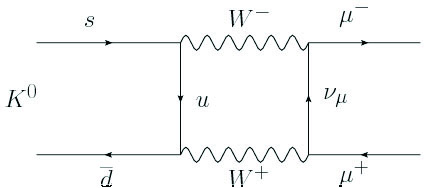
\includegraphics[width=5in]{images/diagram}
    \caption[EPS format diagram. Note: no filetype is designated by adding an extension.]{EPS format diagram. Note: no filetype is designated by adding an extension. The file type is determined and the correct procedure is automatically chosen by xelatex.}
\end{figure}


Quisque malesuada a leo eget ullamcorper. Curabitur ut aliquam quam. Nam quis quam id mauris aliquam blandit porttitor sit amet quam. Donec ut erat eleifend turpis finibus pulvinar.

\subsection{Bitmapped Images Work As Well}

Bitmapped images are a standard file type on PCs, but these files are also usually very large so compressed images may be a better alternative.

\begin{figure}[htbp]
  \centering
    \includegraphics[width=5in]{images/eagle}
    \caption[BMP format drawing. Note: no filetype is designated by adding an extension.]{BMP format drawing. Note: no filetype is designated by adding an extension. The file type is determined and the correct procedure is automatically chosen by xelatex.}
\end{figure}

Morbi hendrerit risus nec quam posuere viverra. Donec quis tellus faucibus, molestie arcu sed, congue urna. Duis eget neque ac libero pulvinar porta eget et magna. Donec a magna eu eros suscipit cursus ac vitae nisl. Vivamus ligula purus, congue sed tortor blandit, ultrices egestas nisl.

\subsection{Not to Mention PDF}

It is often very handy to be able to include a pdf file as an image. By using XeLaTeX this is usually just matter of setting the size, or scale properties correctly.

\begin{figure}[htbp]
  \centering
    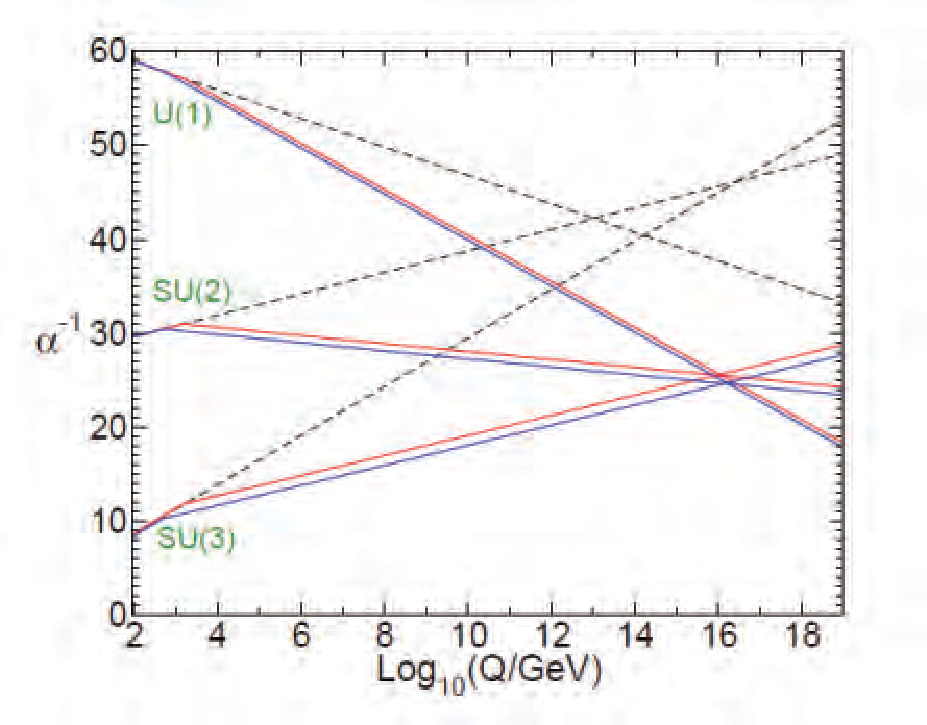
\includegraphics[scale=1.0]{images/graph.pdf}
    \caption[PDF format graph. Note: no filetype is designated by adding an extension.]{PDF format graph. Note: no filetype is designated by adding an extension. The file type is determined and the correct procedure is automatically chosen by xelatex.}
\end{figure}

Nulla mattis augue lacus. Nam non lectus dolor. Cras ac quam vel justo elementum vestibulum. Integer vulputate pulvinar lacus sit amet pulvinar.

\subsection{JPG Is Absolutely Necessary}

For photographs, JPG is the most common format. This format is a fraction of the size of Bit-mapped images and can deliver very good quality at a much smaller overhead. Vestibulum eu lectus vel orci dictum vehicula. Proin id maximus dolor. Integer augue ante, pulvinar ac erat vitae, porttitor ullamcorper libero. \cite{l2012wrinkle}

\begin{figure}[htbp]
  \centering
    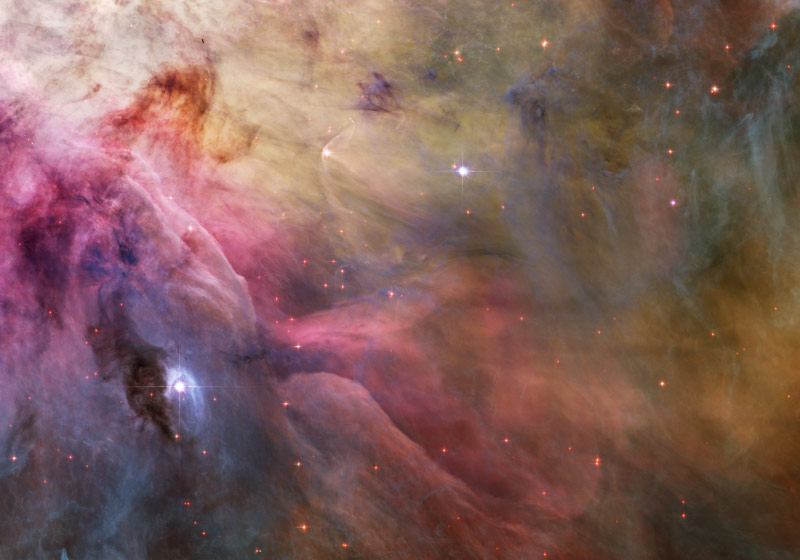
\includegraphics[width=5in]{images/nebula}
    \caption[JPG format image. Note: no filetype is designated by adding an extension.]{JPG format image. Note: no filetype is designated by adding an extension. The file type is determined and the correct procedure is automatically chosen by xelatex.}
\end{figure}

Nunc blandit scelerisque velit, ac facilisis dui finibus et. Sed facilisis tortor vel commodo luctus. Donec est felis, malesuada id nibh in, accumsan malesuada lectus. Sed lobortis volutpat felis, vitae aliquet augue congue id. Fusce ut odio tincidunt, condimentum nulla vel, pharetra arcu.

\subsection{PNGs Will Help Make Files Smaller}

PNG files are even smaller than JPGs and are very good when text and images are combined.

\begin{figure}[htbp]
  \centering
    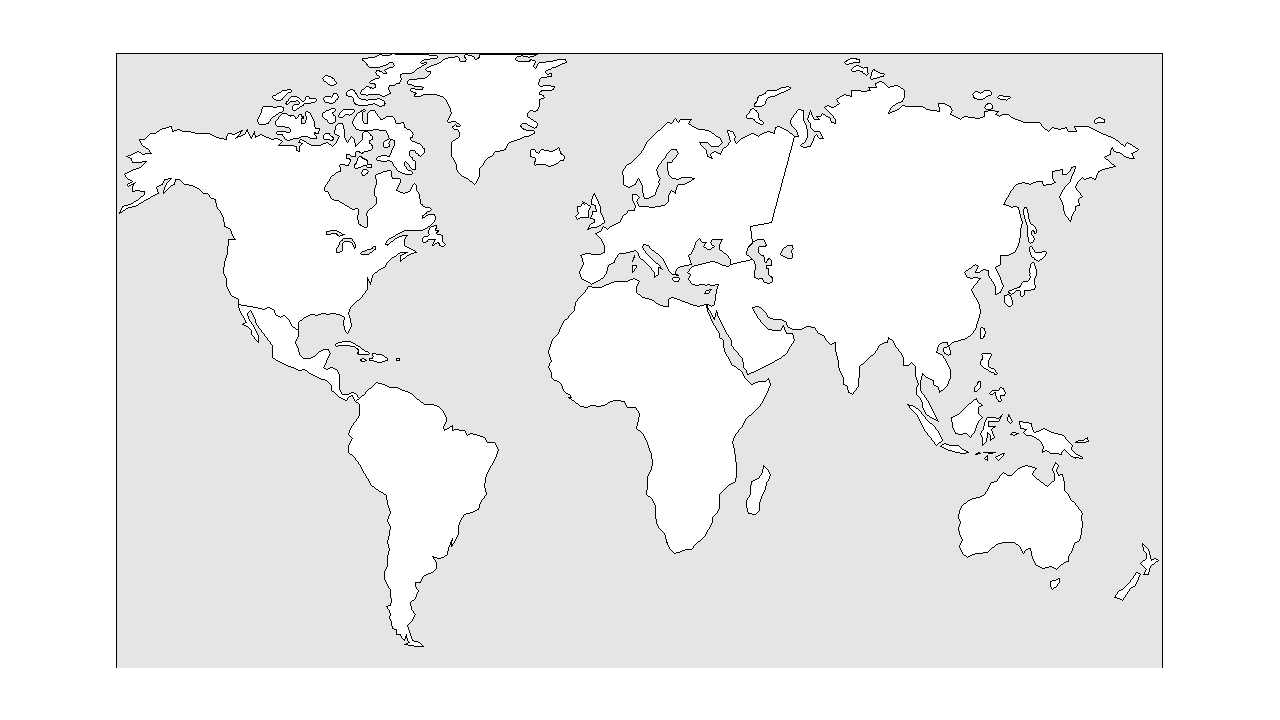
\includegraphics[width=5in]{images/theworld}
    \caption[PNG format map. Note: no filetype is designated by adding an extension.]{PNG format map. Note: no filetype is designated by adding an extension. The file type is determined and the correct procedure is automatically chosen by xelatex.}
\end{figure}



Aenean condimentum libero sed mi porta, tempus ullamcorper lectus venenatis. Aliquam in diam dolor. Maecenas tempus consectetur sem et pulvinar. Aenean aliquam at metus ut hendrerit. Vivamus molestie ac neque eu luctus. Nam convallis maximus quam non lobortis. Fusce sit amet lorem et massa convallis aliquet at sit amet nulla. Suspendisse nec ex elit. Aenean gravida, sapien vitae congue commodo, urna turpis ornare libero, at cursus risus libero in erat. \cite{Rust94}

\section{GIF, TIF, and Others}

Other file formats have not been successful, with or without file extensions. The tests have not been exhaustive so if you have a different type, give it a try. GIF, and TIF both do NOT work at this time. The next image demonstrates how to use multiple images as a single figure. Notice, there is a single caption for ALL figures and that caption starts with a discription of the ENTIRE figure before breaking off into the subfigure descriptions.

\begin{figure}[htbp]
     \centering
   \mbox{
      \subfigure [] {\includegraphics[scale=0.6]{images/mouse}} \qquad
      \subfigure []{\includegraphics[scale=0.6]{images/mouse}} \qquad
     }
    \mbox{
      \subfigure [] {\includegraphics[scale=3]{images/cat}} \qquad
      \subfigure [] {\includegraphics[scale=0.6]{images/mouse}} \qquad
      }
    \caption[Tom and Jerry]{Tom and Jerries. This caption demonstrates how the sub-captions are left out of the List of Figures, but included in the figure itself. A) Tom the first; B) Tom the second; C) Jerry; D) Tom the third.}
    \label{mice}
  \end{figure}


Aliquam mi nisi, tristique at rhoncus quis, consectetur non mi. Phasellus blandit quam ligula, a viverra lacus commodo at. In iaculis nisl vel pretium sollicitudin. In efficitur massa vel elit sollicitudin, vel auctor sapien cursus. Proin feugiat sapien a mi tempus, in consequat augue cursus. Nulla sed sagittis purus. Nunc eu consequat orci, eu laoreet enim. Ut euismod tincidunt sem, eget lacinia dui luctus eu. Aliquam mi augue, faucibus id semper vitae, porta ac ligula. Morbi sed ultrices odio. Mauris id luctus ex. Nulla ac libero dictum, interdum turpis lacinia, scelerisque leo. Praesent varius orci ac eros varius pharetra.



Nunc blandit scelerisque velit, ac facilisis dui finibus et. Sed facilisis tortor vel commodo luctus. Donec est felis, malesuada id nibh in, accumsan malesuada lectus.
\begin{itemize} %
    \item WinEDT: This text editor is recommended for use editing \TeX-files as it has many useful built in macros and is easy to use  %
    \item This program can be found and downloaded here: \url{http://www.winedt.com/} %
    \item The GIMP (GNU Image Manipulation Program) %
    \begin{itemize}%
        \item A freeware graphics editing program for picture editing and file conversions %\vspace{-12pt}%
        \item Comparable to Adobe Photoshop %\vspace{-12pt}%
        \item Can be downloaded here: \url{http://www.gimp.org/}%
    \end{itemize}
    \item A good reference of \LaTeX 2\ensuremath{\epsilon} commands%
    \begin{itemize}
        \item This should be included on the ETD website here: \url{http://etd.helpdesk.ufl.edu/tex.php}
    \end{itemize}
\end{itemize} %


Sed lobortis volutpat felis, vitae aliquet augue congue id. Fusce ut odio tincidunt, condimentum nulla vel, pharetra arcu. In ultricies libero diam, nec rutrum magna vehicula nec. Praesent dictum eros sit amet turpis ultricies, eleifend condimentum dui imperdiet. Donec congue urna ante, id rutrum mi commodo a. Vivamus id tincidunt nunc. Morbi id lacus ut augue ultricies convallis. Duis a lectus quis ante pretium scelerisque nec nec nisi. In id porta justo, at euismod diam. Suspendisse vel tempus arcu. Praesent vel cursus nisi, ac rhoncus odio.


\chapter{MOLECULAR DYNAMICS}
\label{ch:md}
\hfuzz=20pt
\vfuzz=20pt
\hbadness=20000
\vbadness=\maxdimen

Molecular dynanmics (MD) is a simulation approach where the time evolution of a set of interacting atoms is followed by numerically solving their equations of motion.  In MD, the behavior of atoms follow Newtonian mechanics:
\begin{equation}
	  \label{eq:newton_eom}
    \bm{M}\frac{\mathrm{d}^2\bm{R}(t)}
		           {\mathrm{d} t^2}
		=
		\bm{F}(\bm{R}(t))
\end{equation}
where $t$ is time,
$\bm{R} = (\bm{r}_1,...,\bm{r}_{N_\alpha})$ represents the position $\bm{r}_\alpha \in \mathbb{R}^3$ of each atom $\alpha$ for $N_\alpha$ atoms,
$\bm{F} = (\bm{f}_1,...,\bm{f}_{N_\alpha})$ are forces $\bm{f}_\alpha$ acting on each atom,
and $\bm{M}$ is the diagonal mass matrix with the mass of each atom $\alpha$.
The total energy is conserved, even if the kinetic energy and potential energy can change dynamically.

The potential $V$ maps interatomic configurations $\bm{R}$ to provide the potential energy of a system $E_P$.  To evolve a system of atoms, the forces $\bm{F}$ is given by the gradient of the potential for each atom $\alpha$,
\begin{equation}
	\label{eq:calc_forces_from_potential}
	 \bm{f}_\alpha
	 =
	 -\nabla_{\bm{r}_\alpha} V(\bm{R}_\alpha),
\end{equation}
 which can then be substituted into Equation \ref{eq:newton_eom}.

\section{Numerical Integration}
A dynamical simulation computes the trajectory $\bm{r}_\alpha(t)$ of each atom $\alpha$ as a function of time, given the initial position $\bm{r}_\alpha(t=0)$ and velocity $\bm{v}_\alpha(t=0)$.  Since Newton's equation of motion is a 2nd order differential equation, an initial condition needs to specify both positions and velocities of all atoms at the initial condition.

To evolve the equation of motion numerically, time is typically descretized uniformly by incrementing $t$ by the time step $\Delta t$.  A naive implementation of an integration scheme would use the forward Euler algorithm, which is a truncated Taylor series expansion,
\begin{equation}
	\bm{r}(t+\Delta t)
	=
	\bm{r}(t)
	+ \frac{\mathrm{d} \bm{r}(t)}
	       {\mathrm{d}t}
		\Delta t
	+ \frac{1}{2}
	  \frac{\mathrm{d}^2 \bm{r}(t)}
		     {\mathrm{d}t^2}
		\Delta t^2
\end{equation}
This is approach is not time-reversible and suffers from energy drift\cite{allen1987_md}.

A mathematical process is time-reversible if the time reversed process satisfies the same dyamical equations as the original process.  The equations are invariant when e.g. $\Delta t < 0$.  Physically speaking, symmetry of the physical laws under time reversal imples the conversation of entropy.  When the numerical algorithm is not time-reversible then the energy drift is corresponds to a heat flow in or out of the system.

%In molecular dynamics, the Hamiltonian $H$ is seperable, and can be written in the form
%\begin{equation}
%	\label{eq:md_hamiltonian}
%	H(p,q) = T(p) + V(q)
%\end{equation}
%with $T$ being the kinetic energy, $V$ is the potential energy, and $(p,q)$ are canonical coordinates include both the position $q$ and $p$ momentum coordinates.  Here the Euler algorithm is a first order integrator

Instead, molecular dynamics require the use of a numerical integrator that provide better numerical stability and provides time-reversibility.  As an example, we discuss the Verlet integration scheme\cite{verlet1967_integrator}.  While the Euler algorithm is a 1st order forward difference Taylor expansion to order one,  Verlet integration is a 2nd order central difference equation:
\begin{equation}
	\frac{\mathrm{d}^2 r(t)}
	     {\mathrm{d}t^2}
	= \frac{\bm{r}(t+\Delta t)
	          - 2\bm{r}(t)
		        + \bm{r}(t-\Delta t)}
	       {\Delta t^2}
\end{equation}
Thus,
\begin{equation}
  \frac{\bm{r}(t+\Delta t)
	      - 2\bm{r}(t)
				+ \bm{r}(t-\Delta t)}
	     {\Delta t^2}
	=
	- \frac{1}
	       {m}
		\frac{\mathrm{d} V(\bm{r}(t))}
		     {\mathrm{d} \bm{r}}
\end{equation}
\begin{equation}
	\bm{r}(t+\Delta t)
	=
	2\bm{r}(t)
	- \bm{r}(t-\Delta t)
	- \frac{1}{m}
		\frac{\mathrm{d} V(\bm{r}(t))}
		     {\mathrm{d} \bm{r}}
		\Delta t
\end{equation}

\section{Empirical Interatomic Potentials}
%The interatomic potential $U(\bm{R}_i)$ derived from the Born-Oppenheimer approximation is derived from a quantum-mechanical perspective.
The computational cost of \emph{ab initio} techniques such as density functional theory (DFT)\cite{hohenberg1964_dft,kohn1965_dft} can provide accurate structural energies and forces.    \emph{Ab initio} methods are are numerical methods to solvve the elctronic Schr\"odinger equation given the position of the nuclei $\bm{R}$ and the number of electrons.  These calculations provide useful information such as electron densities, energies, and other properties. However, the computational cost to compute $V(\bm{R}_i)$  limits DFT to either static calculations or short simulation times on systems containing a small number of atoms.
An empirical interatomic potential $\hat{V}(\bm{R}_i;\bm{\theta})$ is an analytical function parameterized by $\bm{\theta}=(\theta_1,...,\theta_n)$ which is meant to approximate $V(\bm{R}_i)$, and provide computational efficiency by eliminating electronic structure calculations.

Over the last few decades, a large number of potentials have been developed to descibe various bonding types and environments.
To take representative examples, the Lennard Jones potential\cite{lennardjones1924_lj_pot} was developed for the van der Waals interactions of noble gases, pair potentials such as the Buckingham potential\cite{buckingham1938} can be used for ionic solids\cite{catlow1977_buckingham}, the embedded atom model (EAM)\cite{daw1983_eam,daw1984_eam} was developed for metallic systems,
the Assisted Model Building with Energy Refinement (AMBER)\cite{cornell1995_potential_amber} for biomolecules,
the Tersoff potential\cite{tersoff1988_potential_1,tersoff1988_potential_2} for covalently bonded materials.
To deal with bonding and chemical environments for heterogenous materials like metal/metal oxide interfaces have led to extensions such as MEAM\cite{baskes1992_potential_meam},  REBO\cite{brenner1990_potential_rebo},  COMB\cite{liang2003_potential_comb},
and ReaxFF\cite{vanduin2001_reaxff}.

The topic of empirical potentials and their development is covered in detail in Chapter \ref{ch:potential_development}.

\section{Energy Minimization}

Function optimization is a calculation that pervades much of numerical analysis.  In the context of material systems, the function to be optimized (in this case minimized) is the energy of a system.  The energy landscape of a material may posseses many minima, or conformational substates.  The goal of energy minimization is to find the local energy minimum, which is the atomic configuration corresponding to the bottom of the energy well for that phase.

Physically, energy minimization corresponds to an instantaneous freezing of the system; a static structure in which the forces between atoms have been eliminated at $0 \mathrm{K}$.

Starting with different configuration of atoms, may lead to different energies.  Each of these energies corresponds to a different phase of the material.  The lowest energy phase corresponds to the thermodynamically stable phase at $0 \mathrm{K}$.  Other atomic configurations are non-equilibrium phases of the material system at $0$ K which corresponds to the local minimum of that phase.

\section{Thermodynamic Ensembles}
  The statistical ensembles for molecular dynamics simulations can be defined by examination of the ideal gas law:
  \begin{equation}
  \label{eq:ideal_gas_law}
    PV = N k_B T
  \end{equation}
  where pressure ($P$), volume ($V$), and temperature ($T$), and the number of atoms ($N$) are the state variables of the system.  Each of the state variables is definable in a molecular dynamics simulation.

  The simplest state variables to obtain are the number of atoms and volume.  These are defined by the number of atoms in the simulation cell, and the volume of that unit cell.  Calculation of temperature and its regulation is discussed in Section \ref{sec:nvt_ensemble} through the use of thermostat algorithms.  Likewise, the calculation of pressure is presented with barostat algorithms in Section \ref{sec:npt_ensemble}.

  In MD simulations, it is often necessary or desireable to study a system under the conditions of constant pressure or constant temperature.  The ensembles most typically used for molecular dynamics, are the microcanonical (NVE), canonical (NPT), and isothermal-isobaric (NPT).

  In this section, the NVE is first discussed, and the other ensembles are discussed as modification of the equations of motion for the NVE ensemble.  The purpose of this section is to provide a broad overview of the topic.

Simulations of the canonical ensemble introduce the regulation of temperature.  Problems with temperature rescaling approaches are discussed.  Two types of thermostats are discussed ones involving the stochastic approach of Langevin dynamics, and the Nose-Hoover thermostat\cite{hoover1985_npt} which modifies the equations of motion.

The isothermal-isobaric (NPT) introduces regulation of pressure.  The discussion here is limited to the approach of Parrinello and Rahman\cite{parrinello1981_barostat}.

\subsection{NVE}
Molecular dynamics can be expressed in Hamiltonian form to specifically express conserved quantities\cite{allen1987_md}, which can then be used to derive the equations of motion,
\begin{equation}
	\frac{\mathrm{d} \bm{r}}
	     {\mathrm{d} t}
	=
	\frac{\partial H(\bm{r},\bm{p})}
	     {\partial \bm{p}},
	\quad
	\frac{\mathrm{d} \bm{p}}
	     {\mathrm{d} t}
	=
	\frac{\partial H(\bm{r},\bm{p})}
	     {\partial \bm{r}}
\end{equation}

Integration of the classical equations of motion (e.g. Verlet integration) for a system leads as {$t \rightarrow \infty$} to a trajectory produces an ensemble of microstates: the microcanonical, canonical or isenthalpic ensemble.  Without regulation of temperature or volume, molecular dynamics simulation produces the microcanonical ensemble.

  The independent variables of the microcanonical enseble ($N$, $V$, and $E$) are extensive, which means they should be conserved during the simulation,
\begin{equation}
	\frac{\mathrm{d} H}
	     {\mathrm{d} t}
	=
	\frac{\partial H(\bm{r},\bm{p})}
	     {\partial \bm{r}} \frac{d\bm{r}}{dt}
	+
	\frac{\partial H(\bm{r},\bm{p})}
	     {\partial \bm{p}}
	\frac{\mathrm{d} \bm{p}}
	     {\mathrm{d} t}
	= 0
\end{equation}

  The other state variables are not conserved ($P$, $T$, and the chemical potential $\mu$), and should fluctuate around well-defined average values.


\subsection{NVT and Thermostats}
\label{sec:nvt_ensemble}
The microcanonical ensemble where the energy is kept constant is not often used because this does not correspond with conditions under which most experiments are performed.  Regulation of the temperature is motivated by the need to match experimental conditions and to study temperature-dependent processes,

A canonical ensemble (NVT) is the statistical ensemble that represents the possible states of a mechanical system in thermal equilibrium with a heat bath at a fixed temperature.  The principal thermodynamic variable of the canonical ensemble is temperature.  The ensemble also depends on the number of particles in the system, and the system's volume.

A modification of the Newtonian equations of motion to generate a thermodynamic ensemble at a constant temperature is a thermostat.  Thermostats in molecular dynamics provide a mechanism of regulating the simulation temperature $T_0$.  In NVT simulations, themostating modifies the translation velocity of the particles.

A short discussion of thermostats is provided here.  For a more detailed description, see H\"{u}nenberger\cite{hunenberger2005_thermostat}, Allen and Tildesley \cite{allen1987_md}, and Tadmor and Miller \cite{tadmor2011_md}

In thermostatting, the instaneous temperature $\mathcal{T}$ is compared to the temperature of the heat bath $T$ which the system is coupled to.

The equipartition theorem provides the quantitative prediction, for the average kinetic and potential energies of a system.  The equipartition theorem gives the average values of the individual components of energy.  The average kinetic energy $K$ of a system is related to its macroscopic temperature $T$ through
\begin{equation}
  K
  =
  \langle \mathcal{K} \rangle
  =
  \frac{1}
       {2}
  k_B N_{\mathrm{df}} T
\end{equation}
where $N_{\mathrm{df}}$ is the internal degrees of freedom in the system, $\mathcal{K}$ is the instantaneous internal kinetic energy, and the angular brackets indicate either a time or statistical average over the entire ensemble.
The number of internal degrees of freedom is calculated as $N_{\mathrm{df}} = 3 N - N_c$, for a system with $N$ number of atoms and $N_c$ geometrical constraints on the system.
The instanteous temperature $\mathcal{T}$ is
\begin{equation}
  \mathcal{T}
  =
  \frac{2}
       {k_B N_{\mathrm{df}}}
  \mathcal{K},
\end{equation}
then the average temperature $\langle\mathcal{T}\rangle$ is identical to the macroscopic temperature $T$.  Since the velocity $\bm{v}_i$ of each particle $i$ is obtained from Verlet integration, the instantaneous kinetic energy $\mathcal{K}$ can be replaced by the particles' momenta $\bm{p}_i$,
\begin{equation}
  \label{eq:T_kinetic_energy}
  \mathcal{T}
  = \frac{2}
         {k_B N_{\mathrm{df}}}
    \sum_{i=1}^N
		  \frac{1}{2}
		  \frac{|\bm{p}_i|^2}{m_i}
  = \frac{2}
         {k_B N_{\mathrm{df}}}
    \sum_{i=1}^N
		     \frac{1}{2} m_i |\bm{v}_i|^2
\end{equation}

\begin{equation}
  E_k
	= \langle K \rangle = \sum_{i=1}^N
	=
	\frac{1}{2} m_i |\bm{v}_i|^2
\end{equation}

\subsubsection{Velocity Rescaling}
An obvious way to regulate the temperature is velocity scaling\cite{tadmor2011_md}.  Denote the temperature at time $t$ as $T(t)$ and combine with Equation \ref{eq:T_kinetic_energy}
\begin{align}
  \Delta T(t)
  &= T(t) - T(t-1) \\
  &= \frac{1}{2}
     \sum_{i=1}^N 2 \frac{m_i (\lambda \bm{v}_i)^2}
                         {N_{\mathrm{df}} k_B}
     -
     \frac{1}{2}
     \sum_{i=1}^N 2 \frac{m_i \bm{v}_i^2}
                         {N_{\mathrm{df}} k_B} \\
  &= (\lambda^2 - 1) T(t)
\end{align}
where $\lambda = \sqrt{T/T_0}$.  Thus, the simplest way to control the temperature is to multiply the velocities at each time step by $\lambda$.

This algorithm keeps the instantaneous temperature set to exactly $T_0$.  Since this approach does not allow fluctuations in temperature, it is inconsistent with the statistical mechanics of the canonical ensemble, where we know that the kinetic energy is not constant even when a system is at thermal equilbrium with its heat bath.

Here, we discuss three thermostats for the canonical ensemble: (1) the Berendsen thermostat, (2) the Lagevin thermostat, and the (3) Nos\'e-Hoover thermostat.

\subsubsection{Berendsen thermostat}

The Berendsen thermostat\cite{berendsen1984_nvt} is an algorithm to re-scale the velocities of the particles in molecular dynamics simulations to control the simulation temperature.  Here the temperature of the system is corrected such the deviation exponentially decays with some time constant $\bm{\tau}$
\begin{equation}
  \label{eq:npt_berendsen_1}
  \frac{dT(t)}{dt} = \frac{1}{\tau} (T_0 - T(t)).
\end{equation}
The coupling parameter $\bm{\tau}$ determines how tighly the bath and the system are coupled together.  The change of motion between successive time steps is:
\begin{equation}
  \label{eq:npt_berendsen_2}
  \Delta T(t) = \frac{1}{\tau} (T_0 - T(t)) \Delta t
\end{equation}
This thermostat suppresses fluctuations in the kinetic energy of the system and therefore cannot produce trajectories consistent with the cannonical ensemble.

\subsubsection{Langevin thermostat}

In the Langevin thermostat\cite{allen1987_md}, the regulation of the temperature is maintained by transforming Newton's equation of motion into a stochastic differential equation.
The Langevin thermostat incorporates random forces into the equations of motion.  These random forces model the effect of the heat bath.

The original Langevin equation\cite{langevin1908_equation} described Brownian motion,
\begin{equation}
  \label{eq:langevin}
  m_i \frac{\mathrm{d}^2 \bm{r}_i}
	         {\mathrm{d} t^2}
  =
  - \lambda
	  \frac{\mathrm{d} \bm{r}}
	       {\mathrm{d} t}
	+ \bm{\eta}(t).
\end{equation}
The force acting on the article is written as a sum of a viscous force proportional to the particle's velocity (from Stokes' law), and a stochastic term $\bm{\eta}(t)$, which has a Gaussian probability distribution is correlation function usually expressed as
\begin{equation}
  \label{eq:langevin_eta}
  <\eta_i(t) \eta_j(t')> = 2 \lambda k_B T_0 \delta_{ij} \delta(t-t'),
\end{equation}
where $\eta_i$ is the $i$th component on the vector $\eta_i(t)$.  Equation \ref{eq:langevin_eta} is described in terms of an autocorrelation properties to mathemtically describe Brownian motion.

A description from Brownian motion using probability theory notation\cite{karatzas1991_sde} is clearer than Equation \ref{eq:langevin_eta}. Denote $B(t)$ as a standard Brownian motion, then $B(t)$ has independent increments with respect to time $t$.  For every $t > 0$, the future increments $B(t+\Delta t) - B(t)$, for $u \geq 0$, are independent of the past values $B(s)$, $s < t$.  Brownian motion has Gaussian increments $B_{t+\delta t}-B_{t}$ with mean $0$ and variance $\delta t$; $B_{t+\delta t}-B_{t}~N(0,\delta t)$.
Finally, $B(t)$ has continuous paths and is continuous in $t$.
Since $B(t)$ is nowhere differentiable, the stochastic differential $\mathrm{d}B(t)$ informally denotes the corresponding It\^{o} integral
\begin{equation}
  B(t+\delta t) - B(t)
	=
	\int_t^{t+\delta{t}} \!\!\! \mathrm{d}B(\tau),
\end{equation}
and then $\mathrm{d} B(t)/\mathrm{d}t$ denotes a white noise process.

With this description, $\bm{\eta}(t)$ is based on the evolution of a standard Brownian motion,
\begin{equation}
  \bm{\nu}(t) = \sigma \frac{d\bm{B}(t)}{dt}
\end{equation}
rescaled by $\sigma^2 = 2 m_i \lambda_i k_B T_0$, and $\bm{B}(t) \in \mathbb{R}^3$ with $B_i(t)$ independent from $B_j(t)$ for $i \neq j$.  Then $\bm{eta}(t)$ models the heat flow from a solvent at a constant temperature $T_0$.  The necessary properties implied by Equation \ref{eq:langevin_eta} follow immediately from the definition of standard Brownian motion.

The Langevin thermostat\cite{grest1986_langevin} was originally developed to explain the interaction of the solvent (i.e. the heat bath) on the solute (i.e. the simulated system) and has two levels of interaction.  First, the atoms interact with each other through the interatomic potential.  Second, the atoms are in constant collision with some medium that constitutes the heat bath with the assumption that interactions with the heat bath are more frequent and exert smaller forces than the interatomic iteraction.  This allows the  interatomic interactions to be decoupled from the interactions from the heat bath.  Adding the terms from Equation \ref{eq:langevin} to the Newton's equation of motion, we get the new governing equation for atom $i$.
\begin{equation}
  \label{eq:langevin_eos}
  \frac{\mathrm{d}^2 \bm{r}_i}
	     {\mathrm{d} t^2}
  =
  \frac{1}{m_i} \bm{f}_i
  - \frac{\gamma}
	       {m_i}
	  \frac{\mathrm{d} \bm{r}_i}
		     {\mathrm{d} t}
  + \frac{1}{m_i} \bm{\eta}_i(t)
\end{equation}
where $\gamma$ is now dampening constant associated with atom $i$.

In the Langevin thermostat, the choice $\gamma$ becomes arbitrary.  The choice of too small of $\gamma$ leads to slow equilbrium, while a large value of the dampening constant leads to the stochastic term dominating the equations of motion.

\section{Nos\'e-Hoover thermostat}
% https://www2.mpip-mainz.mpg.de/~andrienk/journal_club/thermostats.pdf
The method to specify the temperature in a molecular dynamics simulation was proposed by Nos\'e\cite{nose1984_npt_1,nose1984_npt_2}.  In this approach, Nos\'e proposed an extended form of the Hamiltonian which introduces a fictitious particle, which couples the system to the heath bath.  The Nos\'e equations of motion are smooth, deterministic, and time-reversible, but stretched the timescale making them impractical for simulation purposes.  These equations were refined by Hoover\cite{hoover1985_npt} to reformulate Nos\'e equations in term of real system variables.  This formulation is known as as the Nose-Hoover thermostat.

The Langrangian equations of motion for the Nos\'e-Hoover thermostat are
\begin{equation}
  \label{eq:nose_hoover_1}
  \frac{\mathrm{d}^2 \bm{r} }
       {\mathrm{d} t^2 }
  =
  \frac{\bm{f}_i}
	     {m_i}
	- \gamma \bm{r_i},
\end{equation}
with
\begin{equation}
  \label{eq:nose_hoover_2}
  \frac{d\gamma}{dt}
  =
  \frac{1}{M}
   \left(
       T(t) - N_{\mathrm{df}} k_B T_0
   \right)
\end{equation}

Equation \ref{eq:nose_hoover_1} is similar to the Langevin thermostat but without the stochastic term.  Since the time-evolution is described by a second order differential equation, the heat may flow to and from the system causing oscillations in the system. Equation \ref{eq:nose_hoover_2} provides the feedback between the $\mathcal{T}$ and $T_0$.

The Nose-Hoover thermostat has one free parameter $M$ which is the mass of the ficticious particle.  This mass serves as mechanism to control the oscillations in the system, as a large $M$ will provide a large inertia and make heat flow between the heat bath and the simulated system sluggish.  If the mass is too small, the thermostat will not control the temperature adequately.

Since the equations of motion have changed, the Verlet integration scheme needs to be modified.

\subsection{NPT and Barostats}
\label{sec:npt_ensemble}
In the isothermal-isobaric ensemble (NPT), the pressure has a specified average value, while the instantaneous volume $\mathcal{V}$ of the system can fluctuate.

The usual approach for the evaluation of pressure $P$ in an MD simulation involves an ensemble average of the instataneous pressure $\mathcal{P}$\cite{allen1987_md}.  For a system with $N$ atoms in a volume $\mathcal{V}$, the instantaneous pressure can be defined as the contributions of each atom $i$
\begin{equation}
  \mathcal{P}
  =
  \frac{1}{\mathcal{V}}
  \left(
    \frac{1}{3}
    \sum_{i=1}^N m_i \bm{v}_i  \cdot \bm{v}_i
    +
    \frac{1}{3}
    \sum_{i=1}^N \bm{r}_i \cdot \bm{F}_i
  \right)
\end{equation}

For a system with interactions, the pressure can be written as virial equation\cite{tadmor2011_md}
\begin{equation}
  \label{eq:virial_equation}
  P
	=
	\left\langle
	  \frac{N k_B T}{\mathcal{V}}
  \right\rangle
  +
	\left\langle
	  \frac{1}
		     {3\mathcal{V}}
    \sum_{i=1}^N
        \bm{r}_i \cdot \bm{F}_{i}
	\right\rangle
\end{equation}
The first term of the right hand side of Equation \ref{eq:virial_equation} is the kinetic contribution and the second term is the Clausias virial function modeling residual contribution arising from atoms interacting through the potential $V$.  Since all quantities to calculate pressure are easily acessible in an MD simulation, Equation \ref{eq:virial_equation} can be used to calculate pressure.  The macroscopic pressure $P$ is simply obtained as $P=\langle \mathcal{P} \rangle$.

The Parrinello-Rahman barostat\cite{parrinello1980_barostat,parrinello1981_barostat} allows the simulation cell to vary in time as a result of the difference between varying the internal microscopic stress tensor and the constant external stress tensor $\bm{\omega}$.  The simulation cell is characterized by the tensor $\bm{H}=(\bm{a}_1,\bm{a}_2,\bm{a}_3) \in \mathbb{R}^{3 \times 3}$, where $\bm{a}_1$, $\bm{a}_2$, and $\bm{a}_3$, are the lattice vectors of the simulation cell.

The discussion provided here follows the exposition by Ray and Rahman\cite{ray1984_npt}.  The Parrinello-Rahman equations of motion can be derived from the Hamiltonian from the coordinate system $(\bm{r},\bm{p})$ to the canonical variables $\hat{\bm{r}},\hat{\bm{p}}$, which incorporates $\bm{H}$,
\begin{equation}
  \hat{\bm{r}}_i = \bm{H}^{-1} \bm{r}.
\end{equation}
$\hat{\bm{r}}_i$ is a position vector in fractional coordinates defined by $\bm{H}$.
\begin{equation}
  \hat{\bm{p}}_i = \bm{H}^T \bm{p}_i
\end{equation}

This allows the box to deform in response to an applied stress, so that the equilibrium shape of the box corresponds to the state where the internal stress is equal to the imposed stress.  Then an extended form of the Hamiltonian which adds the potential energy and kinetic energy associated with the shape of the simulation cell $\bm{H}$, which adds the potential energy due to deformation of the simulation cell and kinetic energy of the box.  The kinetic energy of the box is a ficticious construct which allows the modification of $\bm{H}$ so that simulation cell is in equilibrium with the external stress tensor.

Since the pressure includes a kinetic component due to particle velocities, barostatting requires regulation of both temperature and pressure.
The Parrinello-Rahman equations can be combined with thermostats to then generate the NPT ensemble\cite{shinoda2004_nosehoover} and can then be integrated\cite{tuckerman2006_timeintegrator}.

%Which produces the following Lagrangian from which the equations of motion can be derived.

%\begin{equation}
%  \mathcal{L}
%  \left(\hat{\bm{r}},
%    \bm{H},
%    \frac{d\bm{\hat{r}}}
%         {dt}
%    \frac{d\bm{H}}{dt}
%  \right)
%  =
%  \frac{1}{2}
%  \sum_{i=1}{N}
%      m_i
%      \left(
%				\frac{d \bm{\hat{r}} }
%             {dt}
%      \right)^T
%      \bm{G}
%      \left(
%				\frac{d \bm{\hat{r}} }
%             {dt}
%      \right)
%  - V(\bm{r},\bm{H})
%  + \frac{1}{2}
%    W
%    \mathrm{tr}\left(
%      \left(\frac{d\bm{H}}{dt}\right)^T
%      \left(\frac{d\bm{H}}{dt}\right)
%    \right)
%  - \sigma \mathcal(V).
%\%end{equation}
%Here, $\bm{G}=\bm{H}^T\bm{H}$ and $\bm{W}$ is a constant with the dimensionality of weight that serves as a dampening parameter.

\chapter{Potential Development and Pareto Optimality}
\label{ch:potential_development}

In the previous chapter, an overview of the different computational tools associated with atomistic simulation were presented to give some idea of the interconnectivity and breath of atomistic simulations.  In this chapter, we outline the Pareto approach to potential optimization within the context of more typical current appraoches to potential development.

The purpose is to frame some of the problems in potential development in the proper context so to understand the limitations of typical approaches.  Parameterization is often approached as the minimization of a scalar objective function consisting of the weighted sum of square differences with respect to the prediction of a set of material properties.  When the objective function is convex and continuously differentiable with respect to its parameters, scalar minimization approaches are relatively efficient, even in high dimensions.  For interatomic potentials, these conditions are most likely not guaranteed for even fairly simple formalisms.  When the scalar cost function is not convex, combining derivative-based local optimization procedures with global optimization techniques increases the complexity of parameterization and computational time even for a single selection of a weighting vector.

Moreover, gradient approaches to optimization are not amenable to parallelization.  Local optimization approaches are dependent upon an initial estimate of the optimal parameters and improve the estimate in an iterative manner.  As a result, the parallelization of the computational effort is limited by the dimensionality of the parameter space (length of the computation of the gradient) and limited to the number of simulations required to compute each material property.  This limits the processor utilization to $(M \times N_P)$, where $M$ is the number of simulations required to calculate the cost function, and $N_P$ is the dimension of parameter space.

A larger problem is that weighted least squares approach makes parameterization dependent upon the selection of weights and the choice of the initial condition, both of which heavily influence the final result and must be expressed \emph{a priori}. A potential developer is required to identifty weights before understanding what the trade-off in performance is between alternatives.  Some methods have been developed to pre-determine weights, which incorporate the magnitude ofacceptable errors of the target properties.\cite{martinez2013_fitting}  In practice, a initial choice of weights is made based on the experience of the potential developer, the weights are adjusted, and the optimization procedure repeated.  This process continues in an iterative fashion, until an acceptable parameterization is achieved.

To address the issues of this approach, a novel approach to parameter optimization is taken here which incorporates two pieces.  First, since gradient-based scalar optimization is problematic, we recast the problem as a multi-objective optimization problem (MOO), where each of the sub-objectives in the cost function is treated indpendently.  The concept of a single optimal parameterization is an inappropriate representation, since the improvement in the prediction in one material property generally causes a degradation in the prediction of an other.  Each potential is optimal in its own way, a preference of one over an other is either subjective or dependent upon informatin not encoded into the problem, such as post-selection simulations to predict material properties that it was not optimized for.  Instead, the solution to a MOO is an ensemble of parameterizations; each optimal in its own way.  This set of optimal potentials is defined as \emph{Pareto optimal surface}, and the set of parameterizations which produce these results are the \emph{Pareto optimal set}.  Second, while the Pareto set can be estimated by varying the weights in the cost function in a systematic way, such an approach is in efficient in the presence of local minima.  Instead, we propose that a weight-free, global-minimization approach based upon Monte Carlo sampling is a promising alternative to existing techniques.

This chapter consists of three sections.  In the first section, we introduce the idea of a potential energy surface and how interatomic potentials can be thought of as computationally inexpensive surrogate models; we alsointroduce the terminology of potential development as well as some broad concepts of potential optimization.

In the second section, we build up the notation and terminology of general optimization from a broad mathematical standpoint, first covering the more familiar single-objective optimization.  In particular, we discuss the current techniques to potential optimization which are applied to potential optimzation as well as some of the mathematical problems and issues of this approach.

In the third section, the problem of a parameterization is defined within the context of a MOO problem, with the solution of MOO being the sets of parameters, the Pareto set, which produce nondominated results in objective space, Pareto optimal surface.  When the Pareto surface is convex and continuously differentiable, gradient based approaches can estimate the Pareto surface.  When these conditions do not exist, gradient based approaches produces erroneous results.  As a preview to the evolutionary method presended in chapter \ref{ch:methodology}, we demonstrate how a random sampling based approach to optimization is likely a better approach to estimating a Pareto optimal surface when the potential developer has a high degree of uncertainty to the selection of a region of potential parameterizations or weighting vectors.  This is demonstrated through some sample calculations on the continuous, convex MOO  problem of Schaffer\cite{schaffer1984_pareto} and the discontinuous, nonconvex MOO problem of Kurasawe\cite{kursawe1991_pareto}.

\section{Potential Energy Surfaces}

To study the evolution of a system, such as kinetic process and chemical reactions, it is necessary to calculate the energy for every atomic arrangement of interest.  The potential energy surface (PES) is the energy of a collection of atoms as a function of the positions of its nuclei, $\{\bm{R}\}$.
A PES represents a mapping of the positions of the atoms of a material system to an energies, $V:\{\bm{R}\}\rightarrow E$, with $E\in\mathbb{R}$.
Given an atomic arrangement $\bm{R}$, the evaluated potential surface $V(\bm{R})$ gives the height of the energy landscape for any atomic configuration.
This creates an energy landscape which allows materials systems to viewed from a topological perspective, that the PES can be used to describe the evolution of a system as it moves from one atomic configuration to another atomic configuration.

To describe empirical potentials, we provide with a a mathematical description of configuration space from a crystallographic perspective, and how this crystallgraphic perspective can be translated into other representations common with empirical potentials.

\section{Configuration Space}
\label{sec:configuration_space}
In solid materials, atoms are typically represented as infinite crystalline solids with atomic positions embedded within the representative unit volume.
This representative unit is referred to as a unit cell, which defines that boundaries, the volume, the lattice positions of each atom.

\begin{figure}[ht]
	\centering
  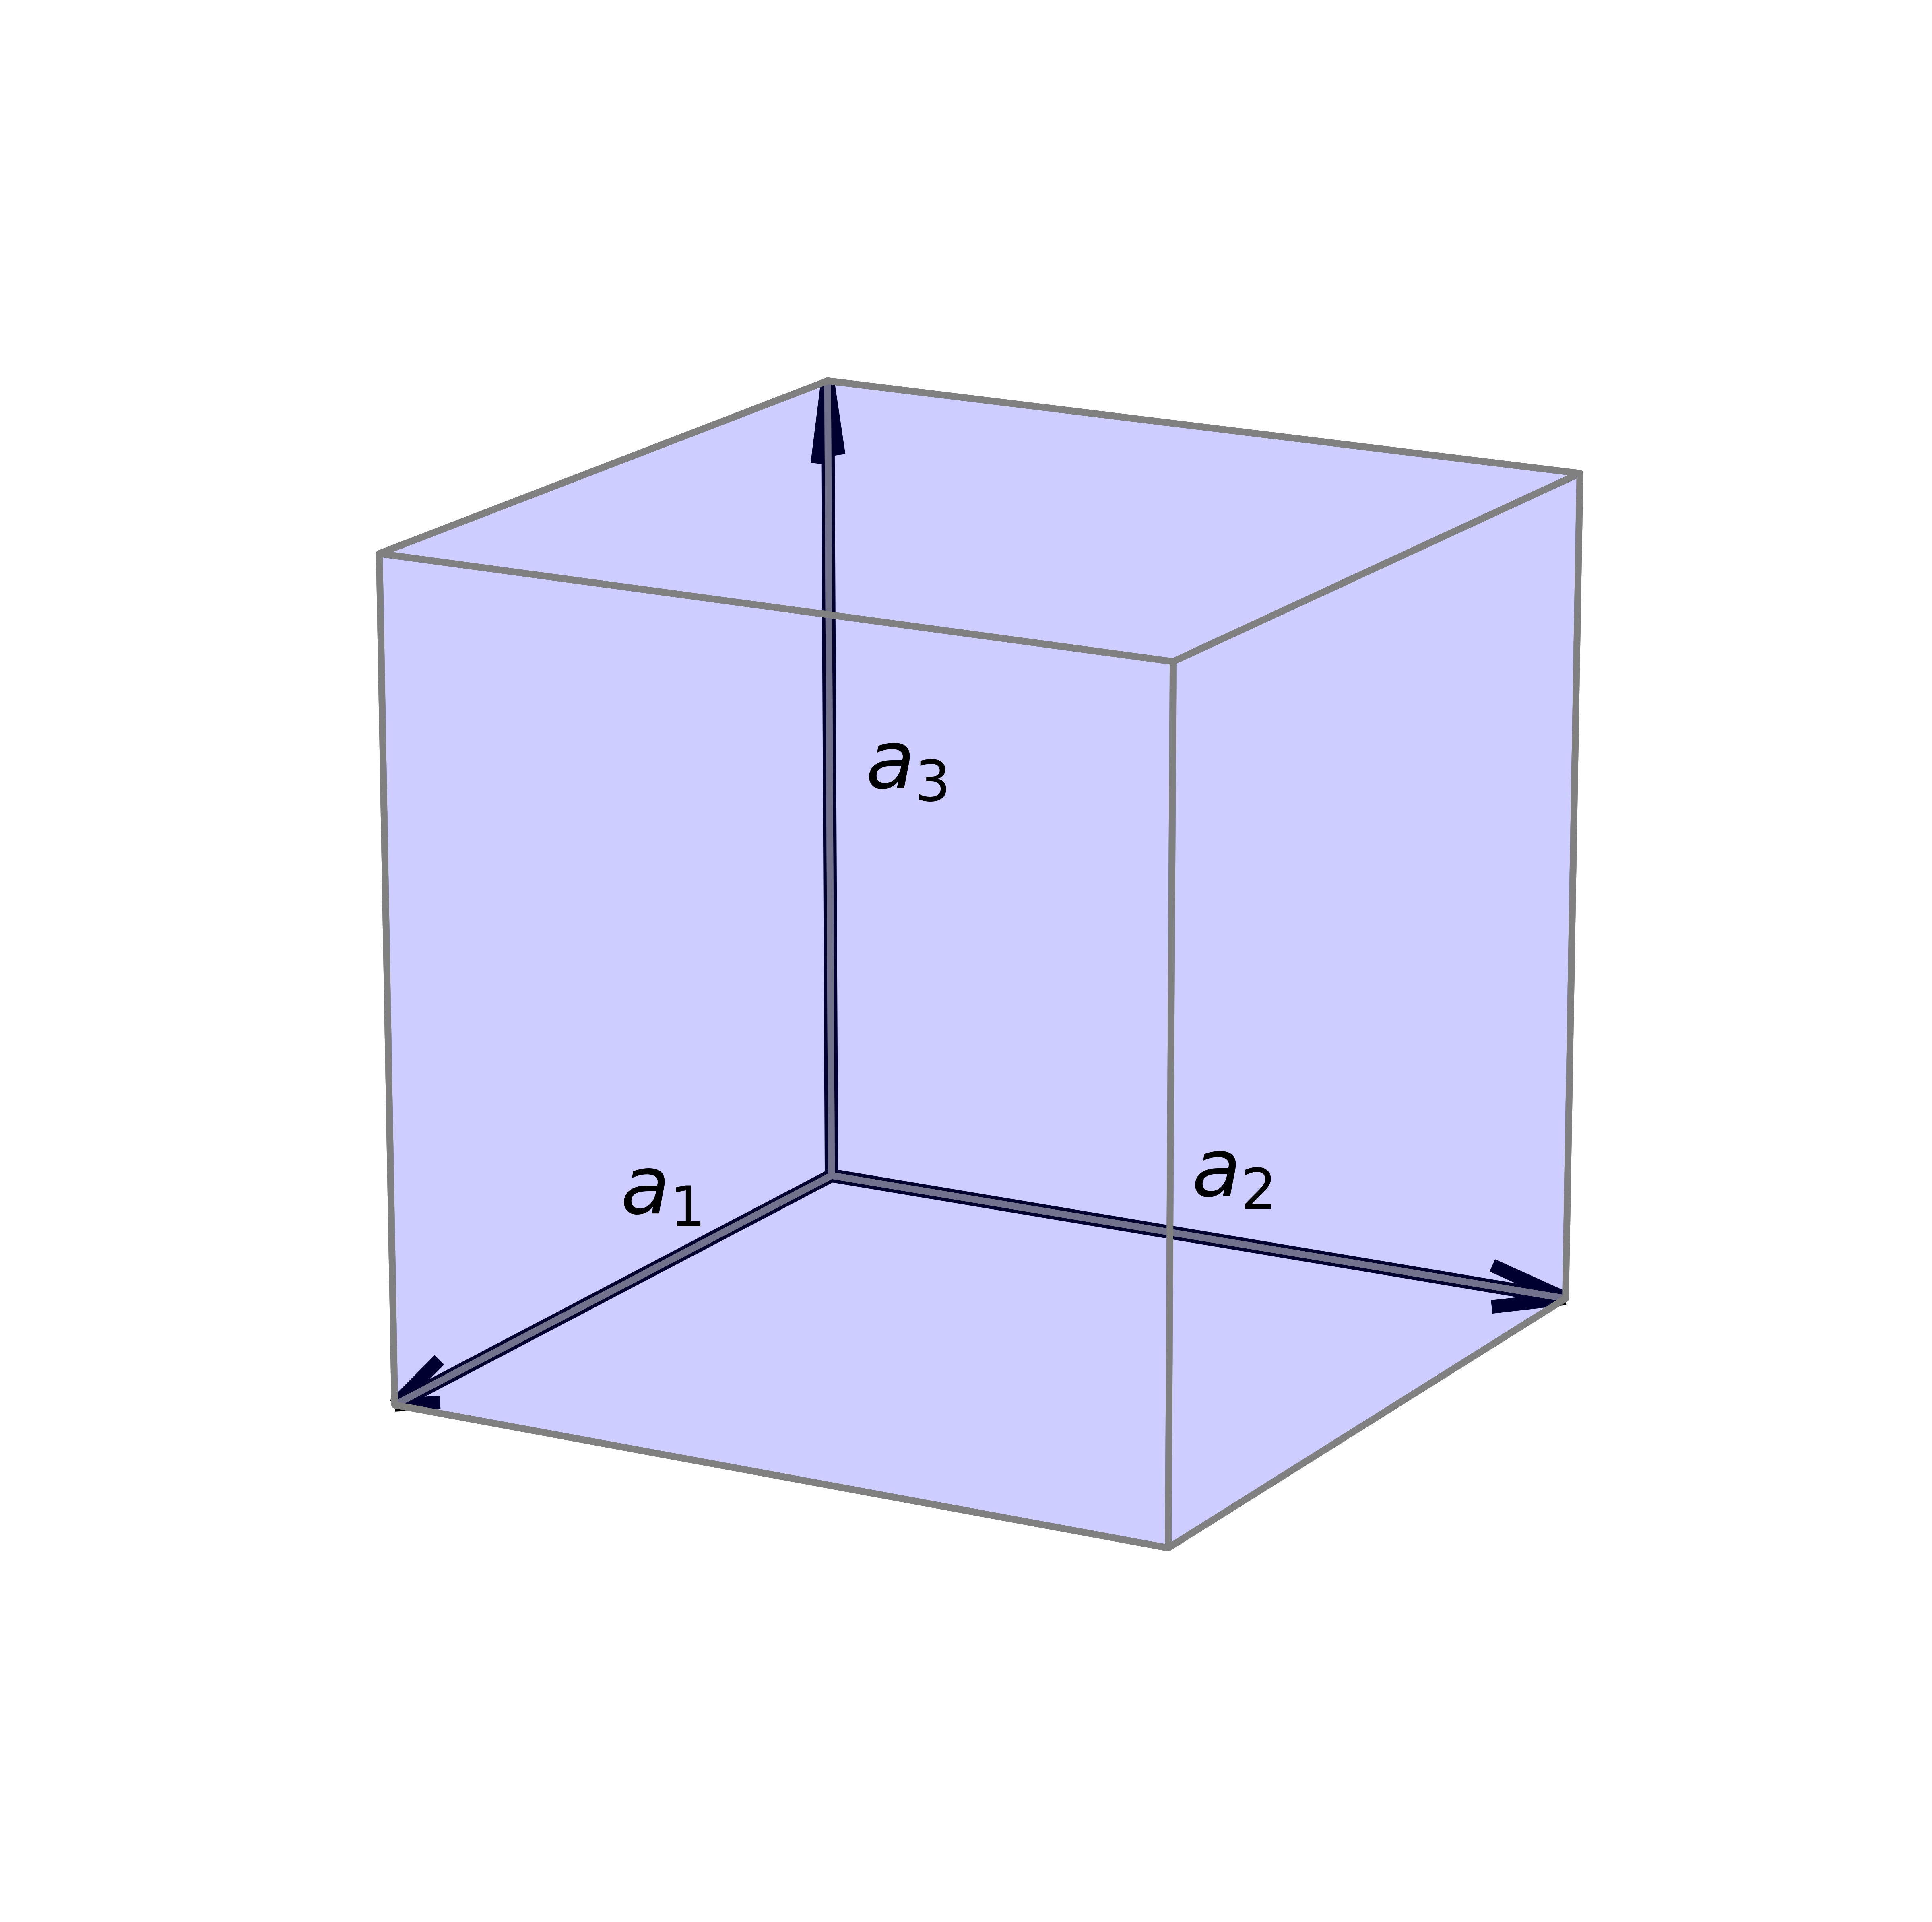
\includegraphics{chapter3/unit_cell}
  \caption{Depiction of the lattice vectors which bound the the unit cell depicted in blew.}
  \label{fig:unit_cell}
\end{figure}

The boundaries of the unit cell are defined are defined by three lattice vectors, defined in three dimensional Euclidean space, $\mathbb{R}^3$.
The three lattice vectors, $\bm{a}_1$, $\bm{a}_2$, and $\bm{a}_3$, with $\bm{a_i}\in\mathbb{R}^3$, define a coordinate sytem in Euclidean space in which to describe a lattice.

To describe the atoms, each atom is identified by a chemical species, $s\in S$, and its atomic position, $\bm{r}$.
If the atomic positions are represented in the Cartesian unit vectors, $[\hat{\bm{\imath}},\hat{\bm{\jmath}},\hat{\bm{k}}]$, then the atomic positions are the ordered triplet, $(r_x,r_y,r_z)$.
More commonly, atomic positions, $(r_1,r_2,r_3)$, are represented in the coordinates system defined by the lattice vectors $[\bm{a}_1,\bm{a}_2,\bm{a}_3]$.  The transformation from the space described by the lattice space to Cartesian space, is described by equation.
\begin{equation}
	\label{eq:fractional_vs_cartesian_coordinates}
	r_x \hat{\bm{\imath}} + r_y \hat{\bm{\jmath}} + r_z \hat{\bm{k}}
	=
	r_1 \bm{a}_1 + r_2 \bm{a}_2 + r_3 \bm{a}_3
\end{equation}

The boundaries of the unit cell describes the periodic boundary conditions, since they also reflect that translational symmetry of the crystalline system.
Each lattice vector can be represented as a translational operator, $T_i$ for ${i\in\{1,2,3\}}$, such that, $T_i(\bm{r})=\bm{r} + n_i \bm{a}_i = \bm{r}$, and collectively,
\begin{equation}
    T(\bm{r}) = \bm{r}
		    + n_1 \bm{a}_1
		    + n_2 \bm{a}_2
		    + n_3 \bm{a}_3 = \bm{r}, \forall n_i \in \mathbb{Z}
\end{equation}

Thus, the geometry for a system with $N$ atoms can be described as
	$\bm{R} = \{\bm{a}_1,\bm{a}_2,\bm{a}_3,\bm{r}_1,...,\bm{r}_N\}$,
	where the $\bm{r}_i$ is defined in an coordinate system defined by the lattice vectors..

\subsection{Empirical Interatomic Potentials}

While the actual PES for any given material system is certainly not analytical, simulations based on solving the Kohn-Sham(KS) equations of density functional theory (DFT) can provide energy calculations of sufficient accuracy for many systems.  However, the computational bottleneck associated in solving for the charge density, energy levels, and wavefunctions of the KS equation limits its adoption as a viable energy calculator to systems consisting of no more than a few hundred atoms.

In contrast, the use of empirical interatomic potentials (EIP) in molecular dynamics simulations can routinely comprise of millions of timesteps on millions of atoms.  In \emph{ab initio} simulations, the solution to the electronic structure of the system is used to calculate the energies of atomic configurations and the forces on the atoms required to evolve the system. In contrast, EIPs have an analytical formalisms consisting of formulae which represent the relevant physics of the system.  This simplification in calculation allows energies and forces drastically improved computational efficiency at the expense of simulation fidelity.

The goal of developing an interatomic potential, $\hat{V}$, is to identify a computationally efficient surrogate model, which models the potential energy surface, $V$.  The use of a hat over a variable indicates that the quantity is an approximation of the actual value.
Since energy is a scalar value, $V$ and $\hat{V}$ are functions in the same space that assigns energies to atomic configuration (e.g. ${V:\{\bm{R}\}\rightarrow \mathbb{R}}$ and ${\hat{V}:\{\bm{R}\} \rightarrow \mathbb{R}})$, we can then define the approximating relationship by the addition of a difference term $\epsilon$
\begin{equation}\label{eq:pes_approximation}
    V(\bm{R}) = \hat{V}(\bm{R}) + \epsilon(\bm{R}).
\end{equation}
In the above equation, $V(\bm{R}$ is the particular energy for a given atomic configuration $\bm{R}$, $\hat{V}(\bm{R}$ is the approximation of the interatomic potential for the same ${\bm{R}}$, and $\epsilon(\bm{R})$ is difference in energies between the two to provide energy balance to the equation.

Interatomic potentials are often expressed as a series expansion of functional terms which explain the relevant physics of a system.  In these cases, the total energy of the system is sum of the individual contribution of each atom $i$.  For a system with $N$ atoms,
\begin{equation}
	\label{eq:potential_energy}
	\hat{V}(\bm{R})= \sum_{i=1}^{N} \hat{V}(\bm{r}_i)
\end{equation}
represents the total energy of a system with $\hat{V}(\bm{r}_i \vert \bm{R})$ being the contribution of the $i$th atom of  a system.
The total energy of a potential of $N$ atoms with an interaction described by the empirical potential, $V$, can be expanded in a many body expansion as described in LeSar\cite{lesar2013_textbook}
\begin{align}
\label{eq:potential_expansion}
	\hat{V}(\bm{R}) &\equiv \hat{V}(\bm{r}_1,...,\bm{r}_N) \\
	          &= \sum_i V_{1,i} (\bm{r}_i)
	             + \sum_i \sum_{i<j} V_{2,(i,j)}(\bm{r}_i,\bm{r}_j)
		     + \sum_i \sum_{i<j} \sum_{j<k} V_{3,(i,j,k)}(\bm{r}_i,\bm{r}_j,\bm{r}_k)
		     + ...
\end{align}
Based upon this expansion, we can classify certain potentials into three classes: pair-potentials, three-body potentials, and many-body potentials.

The first term $V_1$ is the one body term, due to an external field or boundary conditions, which is typically not needed in classical potentials.  The second term $V_2$ is the pair potential; the interactions of this term is dependent the upon the distance between two atoms $\bm{r}_i$ and $\bm{r}_j$, and it is common to represent the distance between the two atoms as $r_{ij}=\lVert \bm{r}_i - \bm{r}_j \rVert^2$.  The three-body term potential $V_3$ arises when the interaction interaction of a pair of atoms is modified by the presence of a third.  In these cases, the pair-potential is typically augmented with three-body terms to express angular dependence, with $\theta_{ijk}$ typically represnting the angle formed by atoms $j$ and $k$ around the central atom $i$\cite{stillinger1985_sw}.    Few potentials employ four body terms due to the dramatic expansion in terms required to describe the interaction.  Instead, a many-body interations is used to reflect the local environment around the atom $i$.

The embedded atom method is a popular approach for modelling metals in molecular dynamics simulations.  In metallic systems, an atom is embedded in a sea of delocalized electron contributed by its neighbors.  To capture this physics, Daw and Baskes postulated an potential which consisted of the pair-wise interactions of the nuclei and an embedding energy term as a function of the host electron density created by all the other atoms in the system.  The EAM model clearly can not be written in the expansion implied by \ref{eq:potential_expansion} without including very high-order terms, but can be represented by a pair-function, an embedding energy function dependent upon the density defined by contribution of a pair-wise density function.

\begin{figure}[h]
  \centering
    \includegraphics[width=5in]{chapter3/lj}
    \caption[The Lennard Jones Potential]{The Lennard Jones potential with $\sigma=1.0$ and $\epsilon=1$, which correspond to the location and depth of the energy well respectively.}
		\label{fig:lj_potential}
\end{figure}

A set of equations, collectively referred to as a formalism, compromises an analytical potential, which decomposes the energy of an atomic configuration into the individual contributions of the terms.
One analytical formalism can be used to describe different chemical compositions with similar underlying physics.  A process of parameterization specializes these functional forms to the specific composition of chemical species, through a process known as parameterization.
If $\hat{V}(\bm{R}:\bm{\theta})$ represents an empirical interatomic potential and is parameterized by a vector of parameters, $\bm{\theta}=(\theta_1,...,\theta_n)$, then $\hat{V}(\bm{R}:\bm{\theta})$ approximates $V(\bm{R})$.

The selection of parameters for the Lennard-Jones (LJ)\cite{lennardjones1924_lj_pot} potential demonstrates simple process for the selection of parameters. The LJ potential approximates the interaction between a pair of neutral atoms, such as a noble gas.  The LJ potential is
\begin{equation}
	V_{\text{LJ}}(r_{ij}) = 4 \epsilon
    \left[
	\left(\frac{\sigma}{r_{ij}}\right)^{12}
	- \left(\frac{\sigma}{r_{ij}}\right)^{6}
    \right].
\end{equation}
The $r^{-12}$ term is repulsive due to the Pauli exclusion principle, which describes overlapping electron orbitals.  The $r^{-6}$ is the attractive long range term, describing the attraction at longer ranges from van der Waals forces.  This equation has two parameters, $\sigma$ and $\epsilon$, which can used to reproduce experimental experimental data or \emph{ab initio} calculations.  As depicted in Figure \ref{fig:lj_potential}, $\sigma$ controls the location of potential well, which is correlated to latttice parameter predictions while $\epsilon$ controls the magnitude of the interatomic interactions, controlling properties like cohesive energy.


\section{Traditional Approaches to Potential Deveopment}

In the typical use of a potential, the parameters are considered to be fixed, $\hat{V}(\bm{R}|\bm{\theta})$, and the function is considered to vary only with respect to the configuration of atoms, $\bm{R}$.  In determing the potential parameterization, the empirical potential is treated as varying due to changing the parameterization, $\bm{\theta}$, while keeping the set of atomic configurations fixed $\bm{R}$.

The process of determining the optimal parameterization, $\bm{\theta}^*$, for $\hat{V}(\bm{R}|\bm{\theta})$ is a process called fitting, which is a process of constructing a curve that has the best fit to a series of data points.  Given an EIP functional form,  the ordinary least squares approach is to minimize the square differences between $\hat{V}(\bm{R}|\theta)$ and $V(\bm{R})$ over configurational space,
\begin{equation}
\label{eq:energy_matching}
	\bm{\theta}^*
		= \argmin_{\bm{\theta}\in\bm{\Theta}}
					\sum_i \left(\hat{V}(\bm{R}_i|\theta) - V(\bm{R})\right)^2
\end{equation}
where $\bm{\Theta}$ being the set of all possible parameterizations and $i$ over all possible atomic configurations.  Since the set of possible atomic configuration $\{\bm{R}_i\}$ is infinite, the interatomic potential has to be developed from a finite set of reference configurations, $\{\bm{R}_i:i<N_{C,F}\}$, which known as the fitting set.  To ensure that $\bm{\theta}^*$ is transferrable to configurations not part of the fitting set, referred to as the testing set, $\{\bm{R}_i:i<N_{C,T}\}$.  For notational convenience, $N_C$ will refer to the number of structures in the fitting set.

\section{Force Matching Method}
Using \emph{ab initio} simulations as the representation of the PES ($V(\bm{R})=\hat{V}_{\text{DFT}}(\bm{R})$), a sequence of atomic configurations can be generated.  Typically, a DFT code is used to calculate energies for the atomic configuration and the interatomic forces for each atom in that atomic configuration. Since both energy and force data are generated in these simulations, the energy matching method described by equation \ref{eq:energy_matching} can be augmented with a force matching method of Ercolessi and Adams.\cite{ercolessi1994_fitting_forcematching}, where they define the objective function,
\begin{equation}
\label{eq:force_matching}
	C_{F}(\bm{\theta}) = \left(3\sum_{k=1}^{N_C} N_k \right)^{-1}
		\sum_{k=1}^{N_K}\sum_{i=1}^{N_k}
			\Vert \hat{\bm{F}}_{ki}(\bm{\theta}) - \bm{F}_{ki}\Vert^2.
\end{equation}
where $N_k$ is the number of atoms in configuration $k$, $\hat{\bm{F}}_{ki}(\bm{\theta})$ is the force on the $i$th atom in set $k$ obtained from the parameterization $\bm{\theta}$, and $\bm{F}_{ki}$ is the reference force from first principles calculation.

In this approach, the fitted potential becomes a surrogate for the potential energy surface estimated by the \emph{ab initio} approach, biasing the parameterization to replicate any errors that may manifest itself due to the first principles method, such as the choice of the exchange correlation functional.  For example, it is well-known that the local density approximation [27] (LDA) calculations tend to result in overbinding causing an underestimate of the lattice constants and an overestimate in the cohesive energies, phonon frequencies and elastic moduli [28].  The generalized gradient approximations (GGA) corrects this error.  The most ubiquitous GGA functional, by Perdew-Burke-Ernzerhof (PBE)[29] is known to overcorrect, as analyzed by Wu and Cohen[30].  Moreover, there is not yet a reliable way to estimate their errors beyond the empirical observation that LDA and GGA results generally span experimental values for many structural and mechanical properties.

The force matching and energy matching approach is popular for the development of modern machine learning potentials which have no functional form, but a complicated mathematical formalism with hundreds of parameters\cite{behler2016_ml_pot} which requires a large number of datapoints to prevent overfitting\cite{wood2018_snap}.

\subsection{Fitting Database}

For analytical potential development, particularly with less complicated functional forms, the computational investment required to acquire such large \emph{ab initio} datasets is unncessary.  Instead, the typical appraoch to potential development is to match the prediction of materials properties to reference values.  In this approach,  potential development comes from optimizing a potential based upon the performance to a fixed set of material properties, known as the fitting database.

In this approach, materials properties are directly related to quantities of interests (QOIs) chosen the potential developer.  The term QOI comes from the field of verification, validation, and uncertainty quantification, where the parametric uncertainty of a model propagates to create uncertainty in the predictions of the QOIs.  Adopting this notation, material properties are denoted  $\bm{q} = ( q_{1},...,q_{N_Q} )$, for $N_Q$ quantities of interest (QOI); the values predicted by a potential are denoted, $\hat{\bm{q}}= (\hat{q}_{1},...,\hat{q}_{N_Q})$.

A fitting database is a collection of structure property functions $q_i$ associated with specific atomic configurations.	The calculation of the $i$th QOI from atomistic simulation tools can be decomposed as a function of energy evaluation of the PES over the $N_{C,i}$ atomic configurations required to do the calculation,
	\begin{equation}
		q_i = q_i(\bm{R}_1,...,\bm{R}_{N_{C,i}}).
	\end{equation}
Likewise, the prediction of the QOI from a formalism, can likewise be denoted as
	\begin{equation}
		\hat{q}_i(\bm{\theta}) = \hat{q}_i(\bm{theta}|\bm{R}_1,...,\bm{R}_{N_{C,i}}).
	\end{equation}
The choice of the more compact notation indicates that once the fitting database is fixed, $q_i$ becomes a static value and $\hat{q_i}(\bm{\theta})$ becomes a function only dependent upon the vector of parameters.

Unlike force matching techniques which require a consistent set of electronic structure data to prevent numerically inconsistent data\cite{behler2016_ml_pot}, a reference value $\hat{\bm{q}}$ can be taken from experiment, calculated from \emph{ab initio} techniques, or integrated from calculations at different levels of theory.  In early efforts of potential development, potentials were developed by fitting to a few experimental numbers.	Due to the increased confidence in DFT calculations, the current trend is to include a significant amount of \emph{ab initio} data.  \emph{Ab initio} data drastically improves the reliability of potentials by allowing the sampling of regions of configuration space, which includes atomic configurations which are difficult or inaccessible experimentally.

Since DFT solve the ground state electronic structure, incorporation of these reference values into the fitting database allows fitting to structural properties which are experimentally difficult to access, such as information from kinetically unstable structures.  The incorporation of first-principles data in the fitting database significantly improves the reliability of semi-empirical potentials by sampling a larger area of configuration space, which discussed in detail in the review article by Payne \emph{et al} \cite{payne1996_dft_database}.

From a computational standpoint, at $0$ K the calculation of material properties become precise because atomic motion stops, and only a single evaluation of a parameterization needs to be evaluated against the reference value.  When the $T>0 K$, time integration through molecular dynamics is necessary to calculate these QOIs.  Shorter trajectories yield incomplete information and confound comparison of parameters with experimental values.  When many $\hat{\bm{q}}(\theta)$ has to be evaluated many times, fitting to structure property relationships which are dependent upon themodynamic ensembles for $T>0$ quickly becomes computational infeasible.

The goal of a fitting database to find to find a representative set of structures in which to calculate the structure property relationships $q_i$.  Since $\hat{q}$ is ultimately detemined from simulations on a series of atomic configurations, we can represent the energy difference between the predicted QOIs and the target QOIs.
\begin{equation}
	\epsilon(bm{\theta})=hat{q}(\bm{\theta})-q
\end{equation}
By choising a set of QOIs, the number of structures in the fitting database is effectively fixed, which reduces the computational investment required to creating the the fitting dataset, when QOIs are determined by DFT.  In addition, the time required to evaluate a parameter set is likewise reduces, an important consideration when $\hat{\bm{q}}(\bm{\theta})$ is evaluated tens of thousands of times. and the time required to determine evaluate a a parameter set again.  The collection of structure property relationships, is denoted $\bm{q}=(q_1,q_2,...q_{N_Q})$ for $N_Q$ structure property relationships.

The determination of the optimal database is a current area of interest.  Zhang and Trinkle\cite{zhang2015_bayes_fitttingdb}.  When the fitting database is defined, potential development then proceeds by the determination of the optimal database.  With the description of the fitting database achieved, our discussion turns on how this potential database can be used to obtain an optimizal parameterization, $\bm{\theta}^*$.

\subsection{Cost Function}
\label{subsec:cost_function}

Typically, the squared difference between the predicted material property values and reference values, $\epsilon_i^2=(\hat{q}_i(\bm{\theta})-q_i)^2$, are used to measure the error since these quantities are analogous to the statistical measure of variance around a mean. The goal of fitting can be described as the selection of a parameter set which minimizes all error terms,
\begin{equation}
\label{eq:moo_LS}
	\min_{\theta\in\Theta}
		  \quad  (\hat{q}_i(\bm{\theta})-q_i)^2,
						\quad i = 1,...,N_Q
\end{equation}

Since analytical formalisms preserve only the salient physics of a particular system, it is inevitable that the potentials will have limitations in their predictive performance caused by the inadequacies of $\hat{V}$ to faithfully replicate $V$.  It is not usually possible to minimize all error terms simultaneously as there are almost inevitably tradeoffs where reducing the error for one quantity of interest increases the error in another quantity of interest.  This problem is a classic problem in multiple criteria decision-making where more than one objective function needs to be optimized simultaneously\cite{miettinen1998_mcdm}.  In fitting interatomic potentials, optimal decisions need to be taken in the presence of trade-offs between conflicting objectives.

One approach to solving this problem is the use of a response data transformation to recast a multi-objective problem as a single-objective problem.  The typical approach is to couple these objective functions with a weighted sum of squares known as the cost function. Thus, instead of multiple objective functions we have a single objective function to minimize
\begin{equation}
	\label{eq:cost_function_LS}
	C(\bm{\theta})=\sum_{i=1}^{N_Q}w_i(\hat{q}_i(\bm{\theta})-q_i)^2
		\sum_{i_1}^{N_Q} \epsilon_i^2(\bm{\theta})
\end{equation}
In this equation, the weights, $w_i$, represent the preferences of the potential designer and effectively serve as the “knobs” which allow control of the parameterization. For example, for the proposed applications of the potential, obtaining precise agreement with the elastic properties may be more important than optimizing the point defect energetics or, of course, vice versa. Although the values of $w_i$ are not explicitly defined in the interatomic potential, $\hat{V}(\bm{R}|\bm{\theta})$, they clearly play a strong role in determining the optimized parameter set.  Since the values of $w_i$ are determined by the potential designer, they are in a sense arbitrary as they reflect subjective preferences upon which the model prioritizes fidelity of one material property at the expense of another.

When $\bm{w}$ is static,  UQ techniques were pioneered by Frederiksen \emph{et al.}\cite{frederiksen2004_md_bayes}, where uncertainty in the paraemters were estimated from $T > 0K$ simulations using \emph{ab initio} molecular dynamics as reference target values with aleatory certainty.  However, as $T \rightarrow 0 K$, uncertainty of the parameters decreases and vanishes to the model fit to the $0K$ reference values.  This should not be surprising as UQ techniques requiree expressing the uncertainty assoicated with each $q_i$ was a probability distribution function.  For $0$ K reference values, the aleatory uncertainty disappears and what is typically left is epistemic uncertainty which cannot be meaningly be quantified as a probability distribution, and expressing the fitting database as point estimates.

Instead, potential developers produce different parameterizations based upon fitting databases based upon similar reference databases.  The real uncertainty in potential development is driven by the choice of $\bm{w}$.  The choice of $\bm{w}$ is nontrivial, considering that this decision must be made \emph{a priori} and the potential developer may not know the implications of adverse changes in prioritizing performance of a potential for a particular material property.

Martinez \emph{et al.}\cite{martinez2013_fitting,martinez2016_posmat} describes an approximation procedure which normalizes the $w_i$ by $q_i$ and multiplies by magnitude of acceptable fractional error.  Starting with an initial estimate of the optimal parameterization $\bm{\theta}_0$ and an initial vector of weight $\bm{w}_0$. an initial parameterization is achieved through a combination of gradient descent and global optimization, resulting on an "optimal" paramaterization, dependent upon the choice of initial conditions, weight preferences, and choice of minimization methods.  Often this result is not acceptable so an \emph{ad hoc} adjustment is applied to the weights, and the process continued iteratively until an acceptable potential is acquired.  Typically, these details are not provided in literature, hindering reproducibility of the potential development process.

When the weighting scheme is used as an \emph{a priori} method, the DM is expected to represent his/her preferences in the form of weights.  Roy and Mousseau (1996) suggests that the role of weights in expressing preferences maybe misleading.  Although the relative importance of weights show the relative importance of the objective functions it is not clear what underlies this notion.  The relative importance of objective functions is usually understood globally, for the entire decision problem, while many practical applications show that the importannce typically varies for different objective function values, that is, the concept is only meaningful locally. (Podinovsky 1994).

Additionally, the minimization of the cost function is no guarantee of transferability.  A potential which is transferable can describe material properties and structures which are different from those it was fitted to.  In some general sense, the issue of transferability deals with the problem of overfitting as well as capturing the relevant physics with the correct functional form.  To assess transferability, a potential needs to adequately describe atomic configurations which are substantially different from those contained in the training set as well as material properties not in the training set.  Moreover, the parameterization of an empirical potential should be relatively insensitive to small changes in weights in the cost function.

\section{Optimization and Pareto Efficiency}

With the typical approach to potential development described, the attention of the rest of this chapter now turns to the development of a more general framework for describing the problem, and the representation of the problem as a Pareto set.  In \ref{subsec:cost_function}, multi-objective optimization was introduced by coupling the many objective function in equation \ref{eq:moo_LS} into a single cost function in \ref{eq:cost_function_LS}.  Adapting the notation of Marley and Arora\cite{marler2004_moo_survey}, the general statement of for the potential parameterization is
\begin{subequations}
	\label{eq:moo}
\begin{align}
  &\min_{\bm{\theta}}	\quad
	  &L_1(q_1(\bm{\theta}),q_1) \\
	&	&L_2(q_2(\bm{\theta}),q_2) \notag \\
	& &... \notag \\
	&	&L_{N_Q}(q_{N_Q}(\bm{\theta}),q_{N_Q}) \notag \\
  &\text{subject to} \quad
	  &g_j(\bm{\theta}) \leq 0, \quad j=1,2,...,N_g \\
	& &h_k(\bm{\theta}) = 0, \quad k=,1,2,...,N_h \\
	& &\bm{\theta} \in \bm{\Theta}
\end{align}
\end{subequations}
where $N_g$ is the number of inequality functions, $N_h$ is the number of equality constraints, and $\bm{\theta} \in \bm{\Theta}$ ensures $\bm{\theta}$ is in the feasible parameter space defined by $\bm{\Theta}$.  Here $\bm{L}_i$ are the loss functions, which are a measures of the information loss of a potential due to the $\epsilon_i$

In MOO literature, the vector $\bm{\theta} \in \bm{\Theta} \subseteq \mathbb{R}^{N_P}$ is a vector of the design variables $\bm{\theta}_i$, for $i=1,...N_P$, and $\bm{\Theta}$ is feasible design space.  $\bm{L}(\bm{\theta}) \in \mathbb{R}^{N_Q}$ are called objectives, cost functions, or criteria.

To find the best parameterization, $\bm{\theta}^* \in \bm{\Theta}$ according to a set of objective functions, which we take here to be a set of loss functions,$\bm{L}=\{L_1,...L_m\}$.  When $m=1$ the problem is a single objective optimization problem and the goal is to minimize a single loss function $f$, i.e.,
\begin{equation}
	\bm{\theta}^* = \argmin_{\bm{\theta}\in\bm{\Theta}} L(\bm{\theta}).
\end{equation}
When $m>1$, the problem becomes a multiple-objective optimization problem(MOO).  In this case, no global optimum exists since the objective functions are competing.

To remove the dependence on \emph{a priori} performance preferences, it is necessary to define an ensemble of parameterization which are optimal in a sense.
Suppose we have two parameterizations,
where $\bm{\theta}_1$ dominates $\bm{\theta}_2$,
denoted $\bm{\theta}_1 \prec \bm{\theta}_2$,
when $\epsilon_i(\bm{\theta}_1) \leq \epsilon_i(\bm{\theta}_2) \forall i \in \{1,...,N_P\}$ and $\exists i \in \{1,...n\}, \epsilon_i(\bm{\theta}_1) < \epsilon_i(\bm{\theta}_2)$.
We say that $\bm{\theta}_n$ is Pareto efficient if $\nexists \bm{\theta}_i \in \Theta, \bm{\theta}_i \nprec \bm{\theta}_1$.

The set of all parameters which produce Pareto effcient points is denoted $\bm{\Theta}^*$, and contains all non-dominated points.  While performance requirements have not yet been encoded to determine $\bm{\theta}^*$, this point must fall in the Pareto set, $\bm{\theta}^* \in \bm{\Theta}^*$.  If $\epsilon_i$ are competing, then clearly there are parameterizations which performs well with respect to $\epsilon_i$, but poorly with respect to $\epsilon_j$.

\subsection{Loss Functions}
Loss function describe the information loss for the $i$th QOI, which is the absolute difference between predicted and target values.  In machine learning strategies, literature will often refer to the its negative, the fitness function, which indicates the system of equations is to maximized rather than minimized.  Through this work, objective functions will be expressed as minimization functions.

The absolute difference function,  $L^1(\bm{\theta})=| \epsilon_i(\bm{\theta}) | = |\hat{q}_i(\bm{\theta}_j-q)|$ for the $j$th parameterization of a potential and has the benefit in that it is in same units as $q_i$.  However, when using gradient techniques, $L_1$ is not continuously differentiable at the area of interest (i.e. where $\epsilon_i =0$), which likely will create numerical instability problems.  In equation \ref{eq:cost_function_LS}, the quadratic loss function
$L^2
		=\epsilon(\bm{\theta})^2
		=(\hat{q}_i(\bm{\theta}_j-q)^2=$
is used, and has the benefits of being a continuously differentiable concave function with respect to $\hat{q}(\bm{\theta})$.  However, the continuity and convexity $L^2$ with respect to $\theta$ is not guaranteed, and is dependent upon to the continuity and convexity of $\hat{q}(\bm{\theta})$ with respect to $\theta$.

The choice of loss functions is critical for cost functions because different different loss functions will give different results given the same weighting scheme.  For examples, a cost function based on $L_1$ will give different results than a function based upon $L_2$.

For the purposes of this work, an acceptable cost function $L$ must be postive and $L$ must preserve the order with respect to $L^1$.  For any two parameterizations, $\bm{\theta}_i$ and $\bm{\theta}_j$, if $|\epsilon(\bm{\theta}_i)| < |\epsilon(\bm{\theta}_j)|$, then $L(\bm{\theta}_i) < L(\bm{\theta}_j)$.

\subsection{Parameter Constraints}

Since analytic formalas respect the relevant physics of a system, then the parameters of the formulae may have physical meaning.  An optimal parameter should represent realistic physics, such as the coefficients of attractive and repulsive terms having the correct sign.  These can be encoded as inequality constraints to enforce $\bm{\theta} \in \bm{\Theta}$.

Moreover, it may also be desirable to impose equality constraints on the parameters.  In charged systems, it is desireable to have charge balance.  For example, for magnesium oxide (MgO), it is necessary to have the charges of the magnesium and oxygen ions to balance, $Z_{\text{Mg}} = Z_{\text{O}}$ to be equal.  These can be encoded as equality constraints.

Finallly, there may be constraints upon QOIs we may want to impose.  For example, the formation energy for the ground state atomic configration (in eV/atom) should be the minimum on the convex hull for competing phases.  Otherwise it would decompose into other compounds with lower energies.  For nickel, the face-cented cubic structure (FCC) is the expected ground state.  In addition to fitting the phase difference between FCC and the competing phase.  It is also desireable to impose the restriction that phase difference is positive.

\subsection{Pareto Efficiency}

To address the problem of weights, a further discussion of Pareto efficiency is necessary. This concept was first introduced by Vilfredo Pareto to model the allocation of resources in an economy\cite{pareto1897_pareto}.  Pareto was the first to realize that cardinal utlity could be dispensed with and be replaced with ordinal utlity\cite{aspers2001_pareto}.  It was not necessary to know how much someone valued a product $X$ or a product $Y$, but only to know that product $X$ is preferable to product $Y$.  As a result, the notion of total aggregate utility to represent the greatest good for the greatest number of people is replaced in modern economic with the notion of Pareto optimality, the idea that a system is maximized when no one can be made better off without making someone else worse off.\cite{mathur1991_pareto}.

In multiobjective optimization problems, it is characteristic that no unique solution exists, but a set of mathematically equally good solutions can be identified.  These solutions are known as nondominated, efficient, noninferior or Pareto optimal solutions.  In MOO literature, these terms are synomous.

Likewise, in the field of potential development the use of a cost function unnecessarily constrains potential development to encode a subjective preference for performance preferences by assigning a vector of weights to correspond with the vector of sum squared errors.  This is ultimately a subjective determination by the potential developer, and the potential developer is ultimately unable to express these preferences \emph{a priori} because knowledge in the relative tradeoffs is necessary to make an informed decision.  Instead of determining $bm{\theta}*$ with a cardinality loss function, which aggregates the subobjective function, one can calculate the Pareto surface to determine $\bm{\Theta}^*$.  Since these potentials are Pareto efficient, the decision then becomes choosing $\bm{\theta}^* \in \bm{\Theta}^*$.

Since all objective functions are to be minimized, a feasible solution $\bm{x}_1$ is said to dominate another feasible solution $\bm{x}_2$, denoted $\bm{F}(\bm{x}_1 \succ \bm{x}_2)$, if and only if $F_i(\bm{x}_1)\leq F_i(\bm{x}_2)$ for $i = 1,...,k$ and $F_j(\bm{x}_1)< F_j(\bm{x}_2$) for at least one objective function $j$.  A solution is said to be Pareto optimal if it is not dominated by any other solution in the solution space.

\begin{figure}[h]
	\centering
  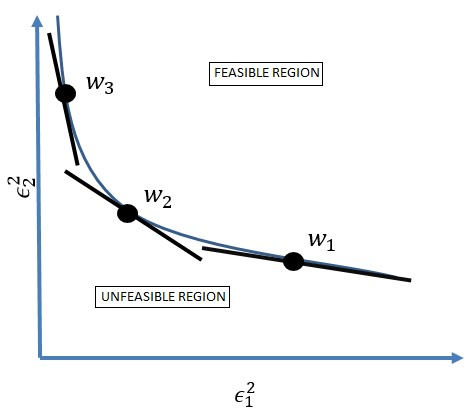
\includegraphics{chapter3/pareto_schematic}
  \caption{Schematic of a Pareto front for the differences, $\epsilon_1$ and $\epsilon_2$, between predicted and actual values for two arbitrary material properties.  The Pareto surface separates regions which are feasible and unfeasible.  Since points in the unfeasible region represent regions of unobtainable accuracy, the Pareto surface forms a boundary of the best possibilities with tradeoffs occurring on the convex hull. }
  \label{fig:pareto_convex}
\end{figure}

Figure \ref{fig:pareto_convex} provides a schematic in 2D, which allows us to illustrate this concept more concretely.  By the definition of Pareto optimality, the Pareto curve separates the feasible region from the infeasible region.  The points $w_1$, $w_2$. amd $w_3$ dominate some of the points on the interior of the Pareto curve, but they do not dominate each other.  The point $w_1$ has better performance with respect to $q_2$ at the expensive of $w_3$, while the fortunes are reserved for $w_3$.  The point $w_2$ is a compromise position between the two.  Without the expression of preferences, one is indifferent to the selection of any of these potentials, but it is rational to choose any of them since they are all Pareto efficient.  If an vector weights was chosen \emph{a priori}, then the potential developer is making a decision about the optimal parameterization without regard to tradeoffs in performance in the fitting set.

The shape of the Pareto front provides valuable insights into the performance of a potential formalism.  In this case, the Pareto front is monotonically decreasing and convex.    Suppose, we start with an initial set of weights $\bm{w}_1$, with the goal of reducing $\epsilon_1$.  A change in the weights to $\bm{w}_2$ places a larger preference on reducing $\epsilon_1$ at the expense of increasing $\epsilon_2$.  Due to the slope of the tangent line implied by the weights, a large reduction in $\epsilon_1$ is possible with only a small sacrifice in $\epsilon_2$.  However, continual improvements in reducing $\epsilon_1$ by changing the weights has a diminishing effect due to the convexity of the Pareto front.  A change in the weights from $\bm_{2}$ to $\bm{w}_3$ will still reduce $\epsilon_1$ at the expense of increasing $\epsilon_2$.  Compared to the previous change, a small reduction in $\epsilon_1$ comes with the tradeoff of a large increase in $\epsilon_2$.

\section{Multiobjective Optimization Methods}
A multi-objective optimization approach should achieve the following conflicting goals as described by Zitzler \emph{et al.} \cite{zitzler2000_moo_evolve}: (1) the best known Pareto front should be as close as possible to the true Pareto front.  Ideally, the best-known Pareto set should be a subset of the Pareto set, (2) solutions in the best known Pareto set should be uniformly distributed and diverse over the Pareto front in order to provide the decision-maker a true picture of trade-offs, and (3) the best-known Pareto front should capture the whole spectrum of the Pareto front at the extreme ends of the spectrum.  While the first two goals are important for multi-objective optimization, the last goal is erroneous.  In potential development, compromise solutions are desireable; a potential with high fidelity with respect to one material property at the expense of a loss of fidelity with respect to all other predictions is pathological.

\section{Solution Methods}
Weights that produce a certain Pareto optimal solution are not necessarily unique, and different weights may produce similar solutions.  On the other hand, a small change in weights may cause big differences in the objective function.  It is not easy for the potential developer to control the solution process because weights behave in an indirect way.  The solution process then becomes interactive, where one tries to guess the weights that would produce a satisfactory solution.  When the tools for potential development to not adequate to support the potential developer in such an \emph{ad hoc} approach, the process leads to frustration and complications in potential development.  In this case, it is advisable to develop a real interactive method where the solution process can be better controlled so that the potential developer can provide more intuitive preference information.

By calculating the Pareto set before analysis and selection, the whole problem of expressing preferences disappears and the traditional analysis approach can proceed in an interactive way.  In addition, provides a wealth of information into all the different rational parameterization, enabling applications such as parametric uncertainty as an input to feed foward to uncertainty quantification methods, shortcomings of potential formalisms, and correlations of errors between computationally inexpensive testing set QOIs to more expensive $T>0$ simulations, which are used to calculate key material properties in engineering applications and larger scale simulations.

\subsection{Pareto Optimization from Cost Function Optimization}

In potential development, the preferences of potential developer influences are particular parameterization, which has the result that the development of empirical potentials is somewhat of a black art.  Here, we demonstrate that the choice of using local optimization tools, as sparsely documented methods for overcoming the weaknesses of local optimization requires considerable skill and experience on the potential developer, as it is difficult to obtain the Pareto surface using traditional techniques.

Let us consider the unlikely case that our potential optimization problem, $C(\bm{\theta},\bm{w})$ is a convex function with respect to $\theta$ and $\nabla C$ being Lipschitz.  Then for an initial condition $\bm{\theta}_0$, we can numerically construct a sequence, ${\bm{\theta}_t}$,
\begin{equation}
	C(\bm{\theta}_{t+1}) < C(\bm{\theta}_{t}), \qquad t = 0,1...
\end{equation}
In each direction, we search in the descent direction informed by the gradient, $\nabla C(\bm{\theta}_t)$ by step size $\eta_t$ to determine $\bm{d}$, the distance to move.  In the gradient descent algorithm, the descent direction is $\bm{d}_t = - \nabla C(\bm{\theta}_t)$.  This process continues until convergence conditons are met to achieve the numerical approximation at $C(\bm{\theta}^*)$.  Any unique vector of weights $\bm{w}$ will result in the optimal parameterization with respect to the selection of weights.  Since $C(\bm{\theta}|\bm{w})$ evaluated at $\bm{\theta}^*$ is a constant, the vector of weights will also define the hyperplane tangent to the pareto surface,
\begin{equation}
	\sum_{i=1}^{N_Q} w_i L_i = C(\bm{\theta}^*)
\end{equation}

In the development of interatomic potentials, the DM is asked to specify weights in which case the method is used as an \emph{a priori} method.
To estimate the Pareto surface, it is sufficient to select a set of weightings.  Since our function is convex and Lipschitz, each unique selection of $\bm{w}$ will give a different point on the Pareto surface as the schematic in figure \ref{fig:pareto_convex}.

The weighting method can be used as an \emph{a posteriori} method where different weight can be used to generate different Pareto optimal solutions, and then themost satisfactory solution selected afterwards.  Systemic methods of perturbing the weights to obatain different Pareto optimal solutions are suggested (Chankong and Haimes 1983), but Das and Dennis 1997 illustrates that an evenly distributed set of weights does not necessarily produce an evenly distributed representation of the Pareto optimal set, even when the problem is convex.
%https://books.google.com/books?id=NHZqCQAAQBAJ&pg=PA1&source=gbs_toc_r&cad=4#v=onepage&q&f=false

The use of local optimization techniques in potential development are clear: local optimization methods are fast, can handle large scale problems, and are largely applicable to a large range of potentials, since they only require differentiability of the objective function and the constraint function\ref{boyd_convex_optimization}.  When Karush-Kuhn-Tucker conditions\cite{karush1939_kkt,kuhn1951_kkt} are met for the constrained optimization parameter optimation problem, solutions remain fairly computationally tractable because of the maturity of the technology and methods associated with gradient based methods and linear algebra techniques.

Algorithms for multiobjective optimization should produce Pareto optimal solutions, and that any Pareto optimal solution can be found.  In this respect, the weighting method has a serious shortcoming.  Any Pareto optimal solution can be found by altering weights only if the problem is convex.  Some Pareto optimal solutions of nonconvex problems cannot be found regardless of how the weights are selected.  In potential parameterization, the compromise is to give up seeking the optimal $\bm{\theta}$, which minimizes the objective over all feasible points.  To solve the problem as a constrained minimization problem with subject to the usual inequality and equality constraints, $g_i(\bm{\theta})$ and $h_j(\bm{\theta})$.  The problems of the weighting schemes have ben explored by the classical potential development community.\cite{martinez2013_fitting}  The method may jump from one vertex to anohter vertex leaving intermediate solutions undetected with relatively small changes in the weighting schemes.\cite{martinez2013_fitting}

Instead, the choice the process is to seek a point that is only locally optimal, which means that it minimizes the feasible points which are near it.  The disadvantages of local optimization methods go beyond not finding the true, globally optimum solution.  The initial guess, $\bm{\theta}_0$ is critical, and can greatly affect the objective value of the local solution.  Little information is provided on how far from the globally optimal solution the local solution is.  In addition, local optimization methods are sensitive to the choice of algorithm, algorithm parameter values, which maybe need to be adjusted based upon the $C$ to $\bm{theta}$ response surface.

One way to overcome the problem with poor initial conditions, is to optimize the cost function from multiple initial conditions.  Given the upper and lower bound of $\bm{\Theta}$ for each parameter $\bm{\theta}$, one can construct an a a grid of initial conditions from which to start the local optimization routine.  As we will demonstrate later, this technique is computationally expensive as the gradient descent paths from each initial condition to achieve optimal solution, $\bm{\theta}^*(\bm{\theta}_0,\bm{w})$, which grows with the density of the grid, the dimensionality of the $q$-space, and the dimensionality of $\theta$-space.

As a result, potential developers have begun to experiment with global optimization techniques, such as genetic algorithms and simulated annealing\cite{martinez2013_fitting,martinez2016_posmat}, to obtain a true global solution of the optimization problem.  However, the compromise in these cases is efficiency.  As the potential formalism increases, the computational complexity of global optimization techniques also increases exponentially.

\section{Pareto Optimization from Monte Carlo techniques}

Genetic algorithms are a popular meta-heuristic that is particularly well-suited for this class of problems.  Traditional GA are customized to accomodate multi-objective problems by using specialized fitness functions and introducing methods to promote solution diversity.  The method which will be proposed in chapter 5 is not a genetic algorithm, but is designed as an evolutionary algorithm which reduces the epistemic uncertainty of parameterization, but evolving the distribution into a distribution  which describes the parameters which produces Pareto optimal results.

The previous section described how the Pareto surface could be estimated for a convex cost function, by selecting an initial condition and solving for the optimal parameterization given set of weights, then repeating the process by varying the weighting scheme.  However, when the cost function is not convex, the process becomes a local solution process and more computationally expensive techniques are necessary.  This can involve assessing multiple starting parameterizations and applying global optimization techniques.  More problematically, much of the information calculated from many evaluations of the cost function other than the final solution (given an initial condition and a weighting vector) is lost.  Even if the information was retained, it is unclear how to integrate that information to more efficiently calculate a Pareto surface.

In a deterministic approach we would want to identify an algorithm such that we start with feasible set of parameterizations and constrains the sets of parameterizations until it produces a set of parameterizations which produces a set of optimal parameters $\bm{\Theta}^*$, which produces Pareto-optimal results $\epsilon$-space.  Here we propose a technique that takes advantage of Monte Carlo sampling.  While Monte Carlo solutions converge slowly, the error of estimamtion decreases as $1/\sqrt{N}$, unlike deterministic search methods that depend expend exponentially on the dimension\cite{caflisch1998_mc}.

The main idea behind this method is that results are based on repeated sampling.  Here we assume that $\bm{\Theta}$ is a random variable, with a probability distribution function which encompasses the information we know about the parameter space.  When we have much information about the parameters, we can use a uniform distribution defined by upper bound and lower bound for each parameter.  Since $\bm{\theta}$ is now a realization of the random variable $\bm{\Theta}$, for each $\bm{\theta}_i$ we can produce $\hat{\bm{q}}_i(\bm{\theta})$ by running these simulations against our simulation machinery.  Moreover, this method is trivially parallelizable.

To determine the estimate $\bm{\Theta}^*$ is determined the following algorithm.  Given the set of QOI evaluations, $\hat{\bm{Q}}=\{\hat{\bm{q}}()\bm{\theta}_1),...,\hat{\bm{q}}_i{\theta}\}$ calculate the Pareto optimal set using the definition of the Pareto optimality, $\hat{\bm{Q}}^* \subseteq \hat{\bm{Q}}$.   The parameters which produce the elements in $\hat{\bm{Q}}^*$, are the set of parameters which produce the Pareto optimal parameters.

The convergence of this algorithm can be drastically improved by updating the probability distribution based upon the results of previous simulations.  In chapter 5, we discuss this process in more detail.

\subsection{Computational and Performance Comparison}
 The performance of these algorithms were tested against the well known problems of Schaffer\cite{schaffer1984_pareto} and Kurasawe\cite{kursawe1991_pareto} to demonstrate the relative performance computational cost of these approaches.  Both of these problem only have two objective functions, which makes visualization of the concepts more concrete.

 awe can produce as many samples to evaluate for performance against the fitting database to produce $\bm{q}.$  When a large enough amount of samples are evaluated,
 It is a generic solution and the iterative approach of generating new populations is akin to previous solutions.
 increases with the increase in the number of objectives.

 The ultimate goal of a multi-objective optimization algorithm is to identify solution in the Pareto optimal set.  However, identifiying the entire Pareto optimal set, for multi-objective problems, is impossible to its size.  Proof of solution optimality is computationally infeasible.  Therefore, a practical approach is achieve successively better approximations of the Pareto surface that represent the Pareto set as well as possible.

 The first of the test optimization function of a smooth convex multi-objective optimization problem described by Schaffer\cite{schaffer1984_pareto}.  Here the multi-objective function $F:\mathbb{R} \rightarrow \mathbb{R}^2$.

 \begin{equation}
 \begin{aligned}[t]
   &\min_{x} \quad
      &\begin{aligned}[t]
            &f_1(x) = x^2 \\
            &f_2(x) = (x-2)^2 \\
       \end{aligned}
 \end{aligned}
 \end{equation}

The second test optimization problem of Kurasawe.
\begin{equation}
\begin{aligned}[t]
  &\min_{\bm{x}}
    &\begin{aligned}[t]
      f_1(\bm{x}) &= \sum_{i=1}^2
          \left[
            -10 \exp\left(-0.2 \sqrt{x_i^2} + x_{i+1^2}\right)
          \right] \\
      f_2(\bm{x}) &= \sum_{i=1}^3 \left[ \vert|x_{i} \vert|^{0.8} + 5\sin(x_i^3)\right] \\
    \end{aligned}
  \\
  &\text{subject to}
    &\begin{aligned}[t]
		      -5 &\leq x_i \leq -5 \\
      		 1 &\leq i   \leq  3 \\
    \end{aligned}
  \end{aligned}
\end{equation}

\begin{figure}[h]
	\centering
  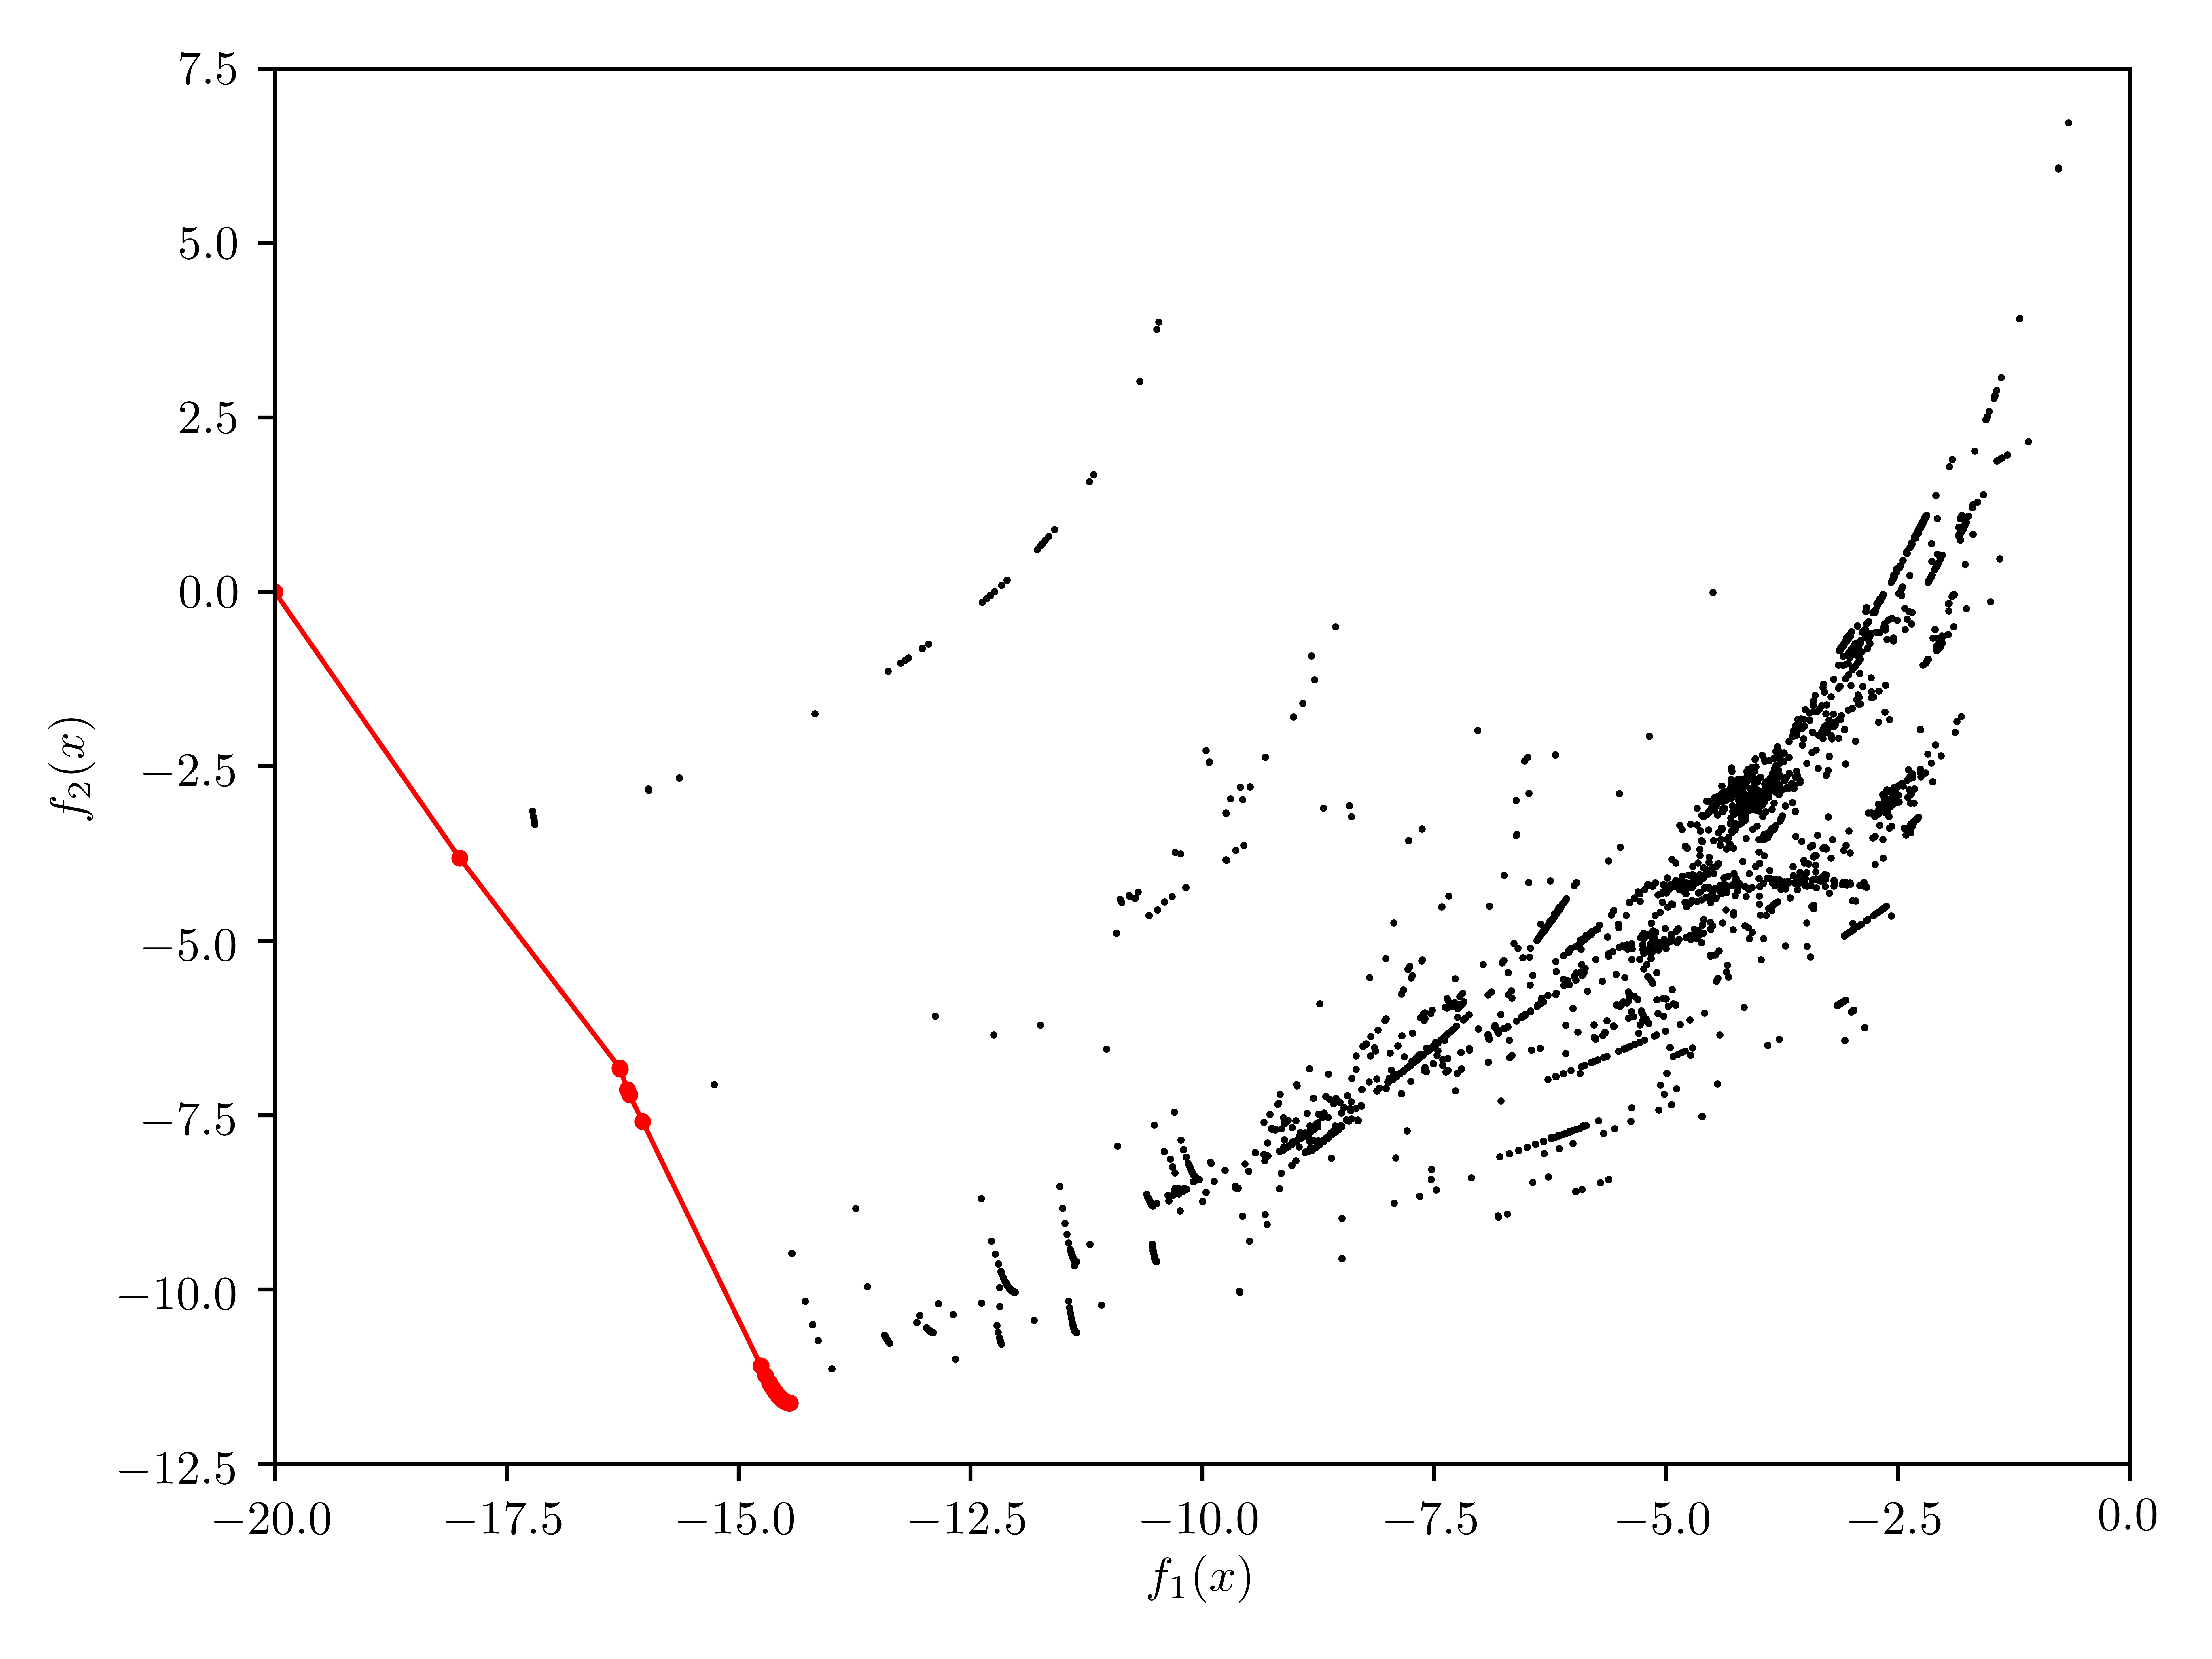
\includegraphics{chapter3/kurasawe_cg}
  \caption{Schematic of a Pareto front for the differences, $\epsilon_1$ and $\epsilon_2$, between predicted and actual values for two arbitrary material properties.  The Pareto surface separates regions which are feasible and unfeasible.  Since points in the unfeasible region represent regions of unobtainable accuracy, the Pareto surface forms a boundary of the best possibilities with tradeoffs occurring on the convex hull. }
  \label{fig:kurasawe_cg}
\end{figure}

\begin{figure}[h]
	\centering
  \includegraphics{chapter3/kurasawe_mc}
  \caption{Schematic of a Pareto front for the differences, $\epsilon_1$ and $\epsilon_2$, between predicted and actual values for two arbitrary material properties.  The Pareto surface separates regions which are feasible and unfeasible.  Since points in the unfeasible region represent regions of unobtainable accuracy, the Pareto surface forms a boundary of the best possibilities with tradeoffs occurring on the convex hull. }
  \label{fig:kurasawe_mc}
\end{figure}

\begin{figure}[h]
	\centering
  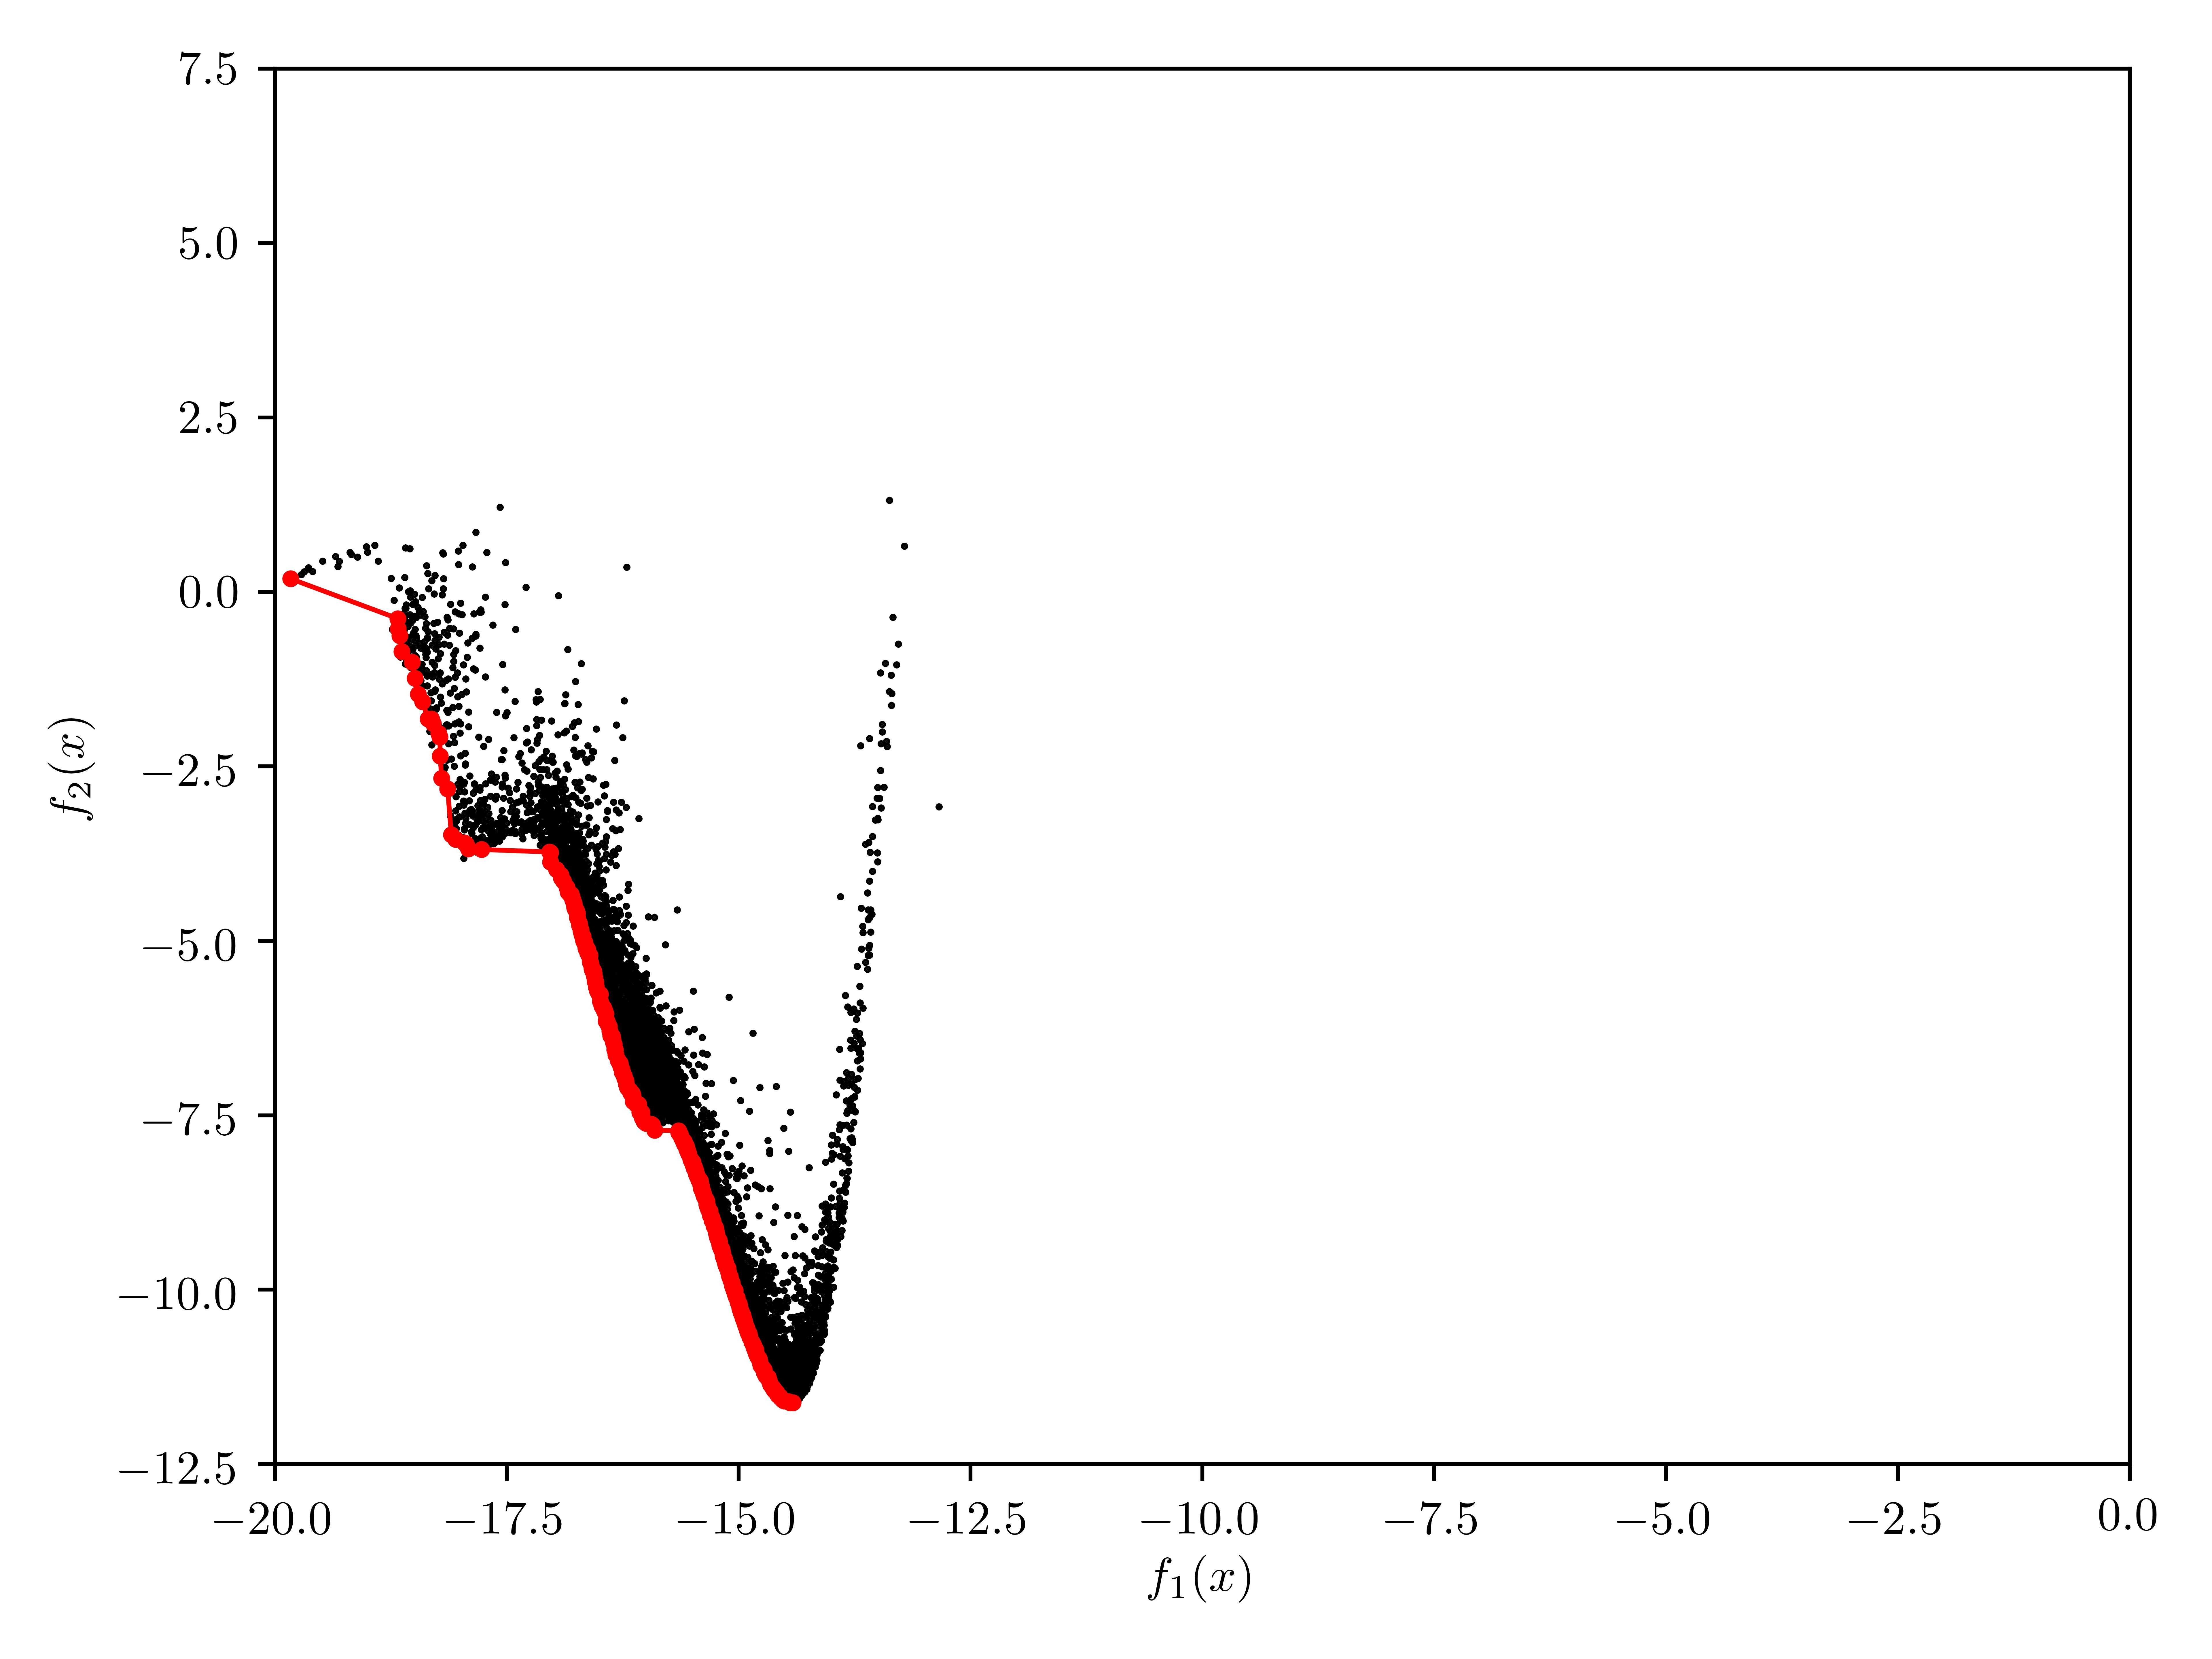
\includegraphics{chapter3/kurasawe_kde}
  \caption{Schematic of a Pareto front for the differences, $\epsilon_1$ and $\epsilon_2$, between predicted and actual values for two arbitrary material properties.  The Pareto surface separates regions which are feasible and unfeasible.  Since points in the unfeasible region represent regions of unobtainable accuracy, the Pareto surface forms a boundary of the best possibilities with tradeoffs occurring on the convex hull. }
  \label{fig:pareto_convex}
\end{figure}

\begin{figure}[h]
	\centering
  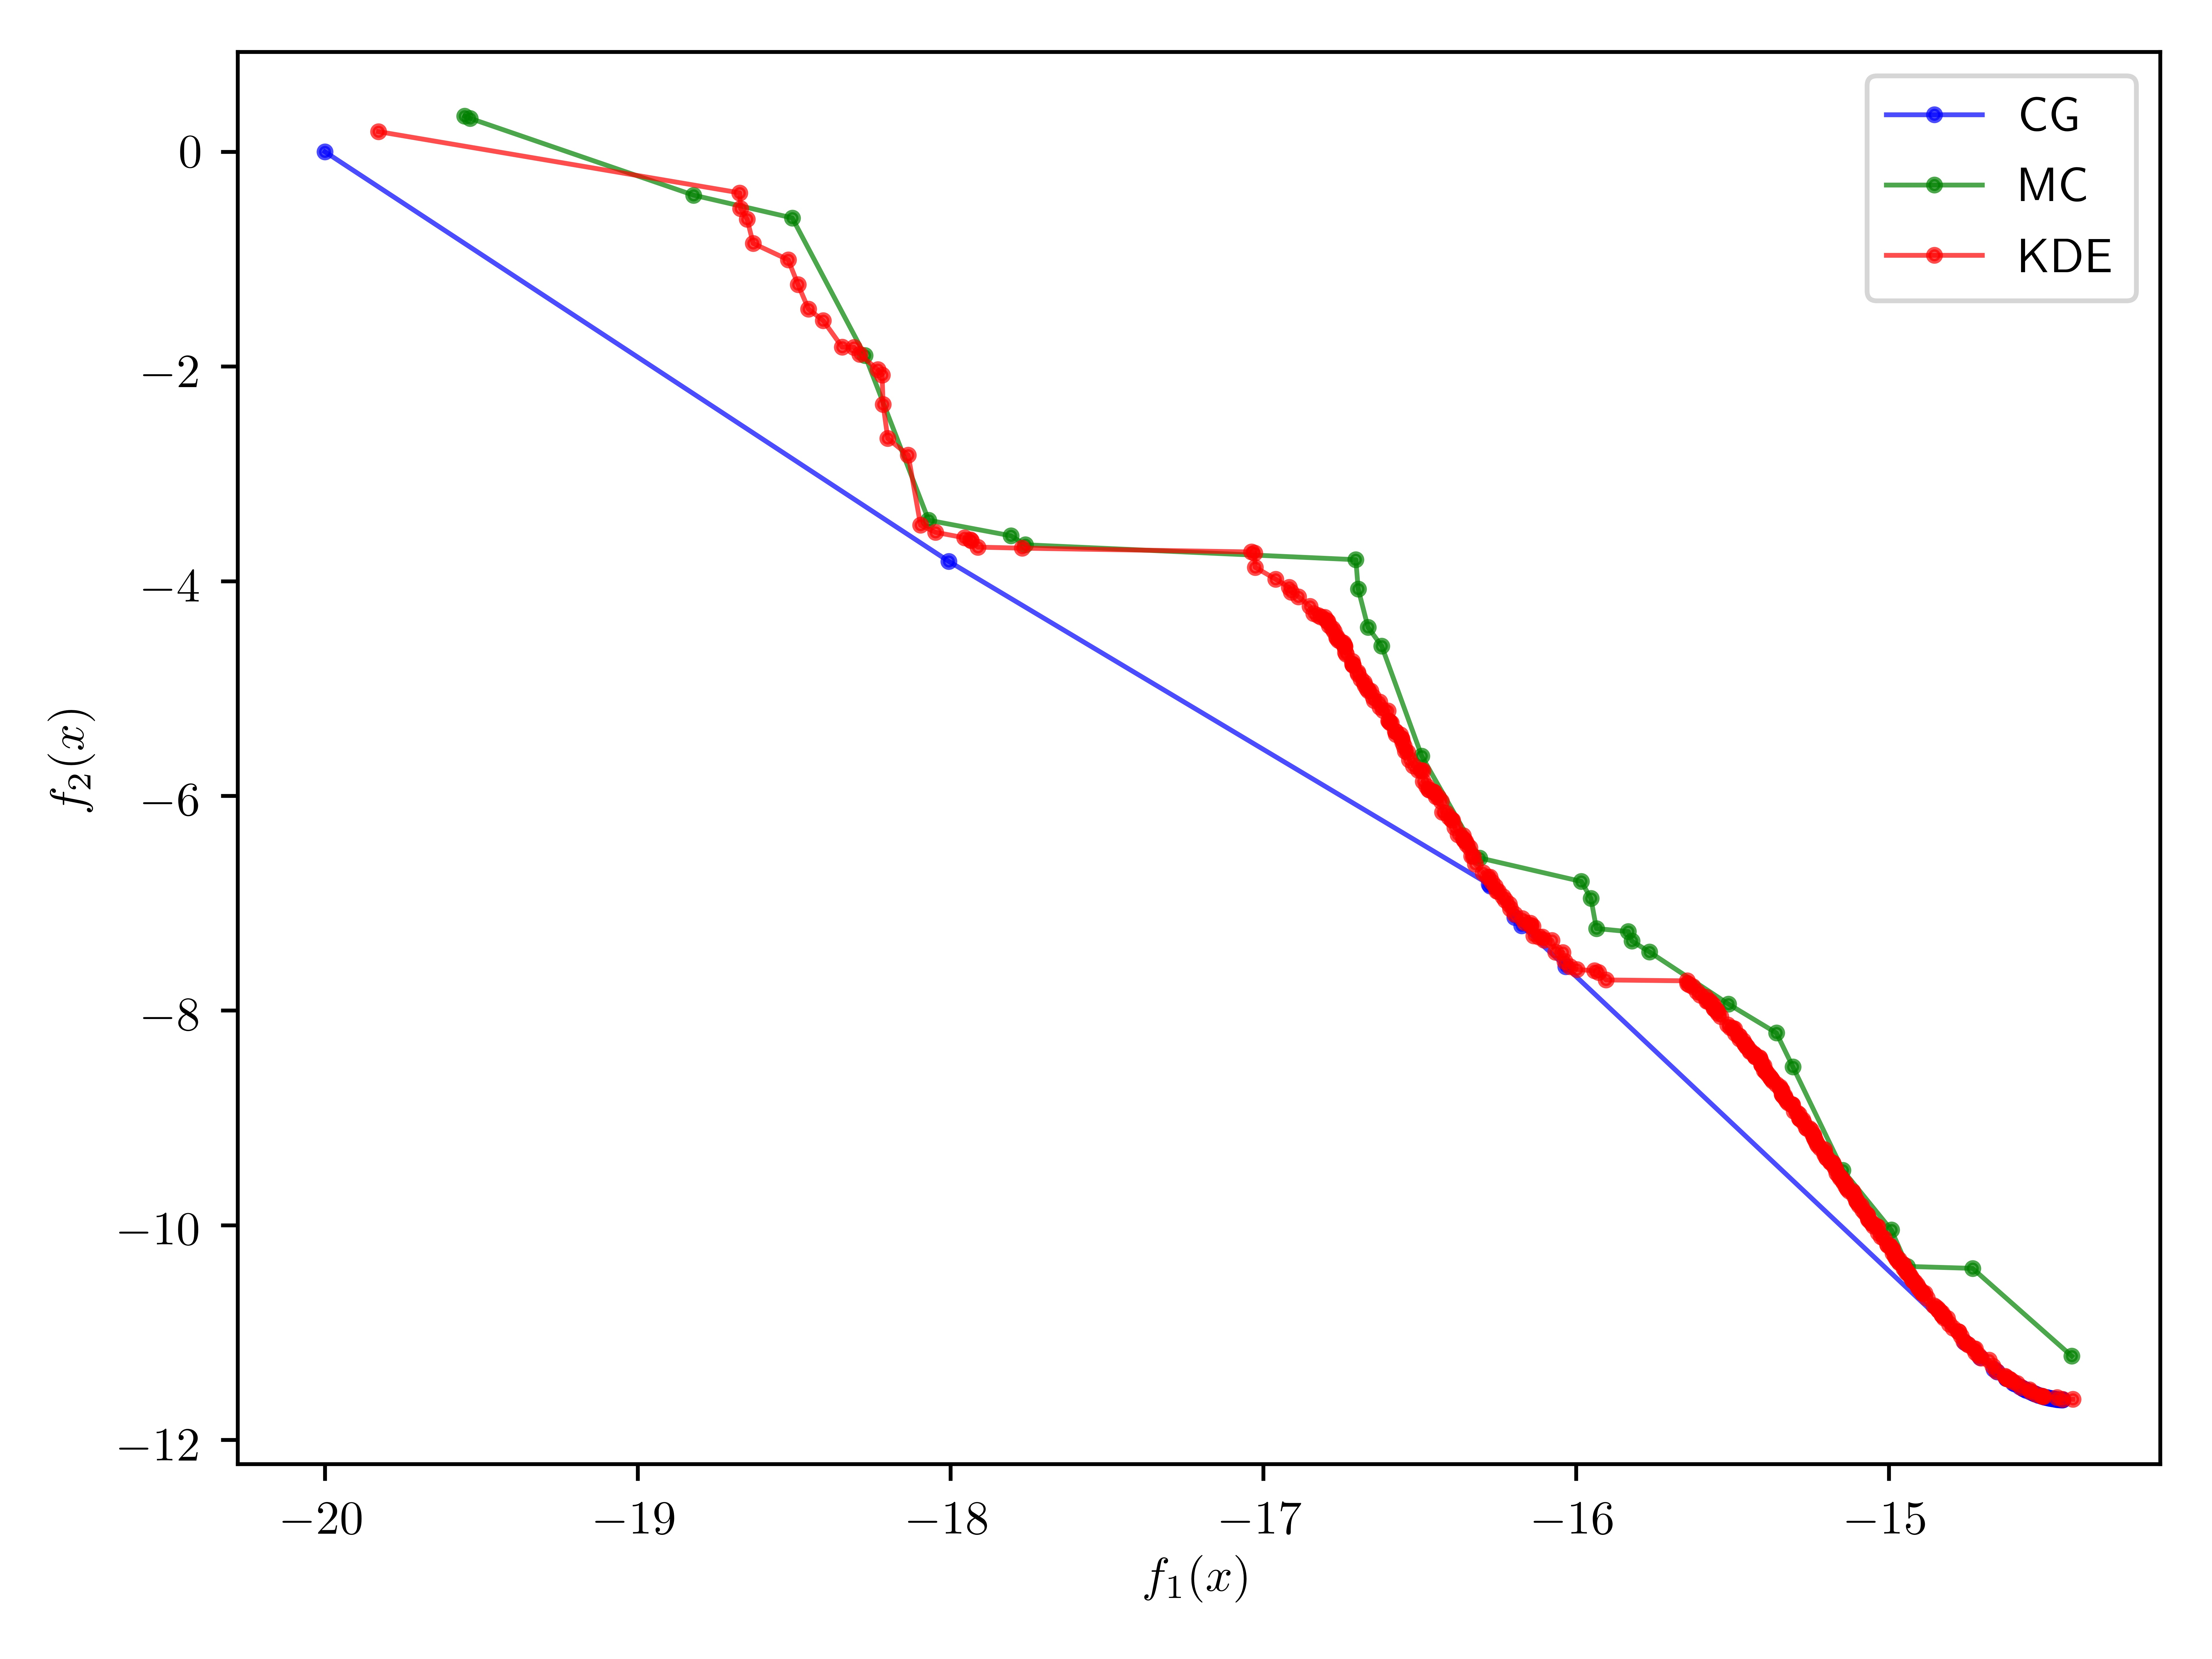
\includegraphics{chapter3/kurasawe_comparison}
  \caption{Schematic of a Pareto front for the differences, $\epsilon_1$ and $\epsilon_2$, between predicted and actual values for two arbitrary material properties.  The Pareto surface separates regions which are feasible and unfeasible.  Since points in the unfeasible region represent regions of unobtainable accuracy, the Pareto surface forms a boundary of the best possibilities with tradeoffs occurring on the convex hull. }
  \label{fig:kurasawe_comparison}
\end{figure}

\begin{table}[ht]
	\caption{Computational comparison between gradient methods and simulation methods against the Kurasawe MOO problem}
	\label{table:kurasawe}
	\centering
	 \begin{tabular}{cccc}
		 \hline
		 d & CG method & MC method & KDE method \\
		 \hline
		 Function Evaluations & 1053132 & 100000 & 10000 \\
 		 Pareto points & 22 & 311 & 508 \\
		 \hline
	 \end{tabular}
\end{table}

\chapter{PROBABILITY METHODS}
\label{ch:probability}

Due to heavy use of simulation methodology involves in this work, a discussion of probability and simulation concepts to clarify terminology and notation.  What follows is a necessarily brief introduction to probability theory in a more rigorous sense, we refer the reader to classic textbooks of Rudin\cite{rudin1987_realanalysis} for a rigorous treatment of measure theory and Chung\cite{chung2001_probabilitytheory} for a measure theory construction of probability.

\section{Probability}
The discussion of the probability methods used in this work starts with the probability construction by Kolmogorov, which builds probability as a measure of sets, but adapted to the particular necessities of probability.

Let $(\Omega,\mathcal{F},\mathbb{P}$ be a measure space with $\mathbb{P}(\Omega)=1$.  Then $(\Omega,\mathcal{F},\mathbb{P}$ is a probability space, with sample space $\Omega$, event space $\mathcal{F}$, and probabilty measure $\mathbb{P}$.  The underlying foundation of any probability  distribution is the sample space, which is the set of all probable outcomes denoted as $\Omega$.  The realization of an outcome is denoted $\omega \in \Omega$.

The events for the measure space are defined in such a way that a probability measure can be assigned.  This allows to assign probability measures on complex events to characterize groups of outcomes.  The collection of all such events is a $\sigma$-algebra $\mathcal{F}$ of subsets of $\Omega$.  Not every subset of the sample space $\Omega$ must be considered an event, the $\sigma$-algebra restricts $\mathcal{F}$ to subsets of $\Omega$ for which $\mathbb{P}$ can be asssigned.

The probability measure, $\mathbb{P}$, a function which maps $\mathbb{P}:\mathcal{F}\rightarrow[0,1]$.  A probability is a real number between zero and one.  Within this work we do not disguish the difference between impossible events which have probability zero, and probability-zero events which are not necessarily impossible.  Events of probability one is an event that happens almost surely, with almost total certainty.

The triplet $(\Omega,\mathcal{F},\mathbb{P})$ is the probability measure space.

\subsection{Probability Measures for Continuous Variables}

\subsubsection{PDF}

\subsubsection{CDF}

\subsubsection{JPDF}

\section{Interpretation of Probabilities}

The meaing of probabilities assigned to potential values of a random variable is not of probability theory itself, but instead related to philosophical context over the interpretation of probability.  In most scientific application, the probability interpretation is physical in nature, in which probabilities are objective and an event's probability is the limit of its relative frequency as the number of samples becomes large.  This interpretation supports the statistical needs and inference requirements for experimental scientists since probabilities can be found by a repeatable objective process (e.g. experiments), and are thus devoid of opinion.  Within this context, probabilities are \emph{aleatory}.  Uncertainty is irreducible and inherent to to the physical process observed.

For finite temperature simulation above $0$ K, molecular dynamics simulations allow sampling from themodynamic ensembles.  Although the simulations are replicable since time-integration and the empirical potential are deterministic.  Sampling from the time-series or by randomly assigning initial velocities, allows molecular dynamics to model aleatory uncertainty associated with a model.

Within this work, probabilities are evidentiary and can be assigned to any problem statement, even when no random process is involved, as a way to represent subjective plausibility, or to the degree in which the statement is supported by available evidence.  Evidential probabilities here are considered to be degrees of belief, such as the Laplace interpretation where probabilities are defined in disposition to gamble at certain odds\cite{laplace_probability}.  Here, conherent subjective belief systems follow the laws of probability\cite{ramsey_probability,definetti_probability}.  Here, uncertainty is \emph{epistemic} and is based on current evidence, but is mutable based upon receiving new observations\cite{ramsey2016truth,definetti1980_foresight,jaynes2003_probability}.  This philsophical interpretation is more closely associatiated with Bayesian inference.

In practice, the uncertainty associated with any problem has both \emph{aleatory} and \emph{epistemic} components.  Within this context, the field of uncertainty quantification\cite{oberkamph} in involved the quantitative characterization and reduction of uncertainties in both computational and real world applications.  The difficulty of applying Bayesian frameworks to potential development is the evidence is constrained to the size of the dataset, a parameterized potential likely produced biases due to the inevitable tradeoffs in assigning preferences in predicting various material properties.  Moreover, the inability to define the uncertainities associated target properties frustrates standard VVUQ and Bayesian approaches.

 Neither of these interpretation is particularly useful for our application.  Here, the probability distribution should be interpreted as propensities.  In the propensity theory of probability, is the probability of an event to produce an outcome of a certain kind, or to yield a long-run relative frequency of such an outcome.  Propensities are not relative frequencies, but the purported causes of the observed stable relative frequencies.

Regardless the choice in the interpretation of the meaning of probabilities, the mathematics works the same.

Formally, a continuous random variable is a random variable whose cumulative distribution function (CDF) is continuous everywhere\cite{bertsekas2002_probabilitytheory}.  More practically, random variables of interest can be defined by a probability density function (PDF), which characterize the CDF.

\section{Random Variable}
A random variable $X$ is a variable whose possible values are outcomes of a random phenemon.  As a function, a random variable is required to be measurable, which rules out pathological issues.  A random variable has a probability distribution, which specificies the probability falls in.  Specifically, $X:\Omega\rightarrow\mathbb{R}$.  If a random variable $X:\Omega \rightarrow \mathbb{R}$ is defined on the probability space $(\Omega,\mathcal{F},\mathbb{P})$.  Then the probability of an event $A$ occuring is $\{\omega:X(\omega)=A\}$ which is denoted as $\mathbb{P}(X=A)$.

Formally, a random variable is particular type of measurable function.  However, there is an important difference which maybe more philosophical than mathematical due to the difference in the underlying domains.  A random variable operates on a set of outcomes or processes defined by $\Omega$, while deterministic variables does not.  This isn't a mathematical difference as the underlying domains are just sets, and the $\sigma$-algebra and measures provide the relevant mathematical structure.

For a probability space, even if a specific random process isn't mentioned, there is an implied assumption that such a random process exists.  Otherwise, there would be no need for probability to have its own language.

A random variable can only be evaluated by performing an unpredictable experiment.  That is, you don't choose which $\omega \in \Omega$ to choose.  If you did choose a specific $\omega$, the you aren't evaluating a random variable, you're just evaluating a measurable function.

\subsection{Expectation of a Random Variable}

If $X$ is a random variable with a finite number of outcomes, $\{x_1,x_2,...,x_k\}$ occurs with the probabilities $\{p_1,p_2,...p_k\}$.  Then the expectation of $X$ is defined as
\begin{equation}
  \mathbb{E}[X]=\sum_{i=1}^{k}x_i p_i
\end{equation}
If $X$ is a continuous random variable, then
\begin{equation}
  \mathbb{E}[X]=\int_{\Omega} X(\omega) d\mathbb{P}(\omega)
\end{equation}
If $X$ admits a density $f(x)$, then the expected value is defined as
\begin{equation}
  \mathbb{E}[X]=\int_{\mathbb{R}}x f_{X}(x) dx
\end{equation}

\subsection{Functions of Random Variables}
A new random variable can be defined by applying a measurable function to the outcomes of a a real-random variable $X$.  That is $Y=f(X)$.  Then the cumulative distribution of $Y$ can be defined as $F_Y(y)$
A probability density function for a random variable $X$ has a density $f_X$, where $f_X$ is a non-negative function:
\begin{equation}
  \mathbb{P}[a \leq X \leq b]=\int_{a}^{b}f_{X}(x)dx
\end{equation}

\subsection{Sampling a Random Variable}

In this section, we discuss the general concept of sampling using the technique of inverse transform sampling as a method for pseudo random number generation.  Inverse sampling samples from a uniform distribution, $u_i=U(0,1)$, and interprets it as a probability, and then returns the largest number x from the domain of the distribution $\mathbb{P}(X)$ such that $\mathbb{P}(-\infty<X<x) \leq u_i$.

Computationally, this method involves computing the CDF and inverting the function, which is known as the quantile function.

Note that for a discrete distribution, computing the CDF is not in general too difficult: we simply add up the individual probabilities for the various points of the distribution.  For a continuous distribution, however, we need to integrate the probability density function (PDF) of the distribution, which is impossible to do analytically for most distributions (including the normal distribution).

\subsection{Multivariate Sampling}
\label{section:multivariate_sampling}

\section{Estimating Probability Distribution Functions}

\subsection{Parameteric Distributions}

\subsection{Non-parameteric Distributions}


\subsection{Bayesian Inference}
\label{section:bayes}

Let $\hat{\bm{X}}$ be a sample population with the observed data points, $\hat{x}_i \in \hat{\bm{X}}$.

The \emph{prior distribution} is the probability distribution before any data is observed.  If $\bm{\theta}$ is a vector of parameters for the distribution of $X$.   Since this distribution is dependent upon \emph{a priori} information, the prior distribution might not be easily determined.  In this case, a non-informative distribution can be used to as an initial estimate, which is updated based upon newer observations.

The \emph{sampling distribution} is the distribution of the observed data conditional on its parameters, $f(\bm{X})$

\subsection{Uninformative Distributions}
\label{section:bayes_prior}
A prior proabability distribution of a certain  quantity is the probability distribution that would express one's beliefs about this quantity before some evidence is taken into consideration.

Since the posterior density $f_{post}$ is proportional to $L(x)f_{prior}$, the maximimum likelihood will match the maximum posterior if the maximum of the likelihood is a maximum of the prior distribution.  Since a uniform prior means that the prior is constant, we get that the posterior is proportional to the likelihood, so they have the same maxima.

An in-depth discussion about the choice of uniform priors are

\section{Density Estimation}

\subsection{Parametric Estimation}

If $X$ is a random variable, then a parametric model for the probability distribution function of $x \in X$ implements are restricted set of functions, $f(x;w)$, where $w$ are the parameters of the probability distribution function $p(x)=f(x;w)$.

This work only concerns itself with with two parametric probability distribution functions: the uniform distribution and the multivariate distribution function.  The uniform distribution is defined by the lower bound $a$ and the upper bound $b$ of the probability distribution function, which is constrained by its use to define an uninformative prior distribution to incorporate \emph{a priori} information.

Maximum Likelihood Estimator

The second probability distribution is the Normal distribution, where the MLE estimators for is the meand and variance.

The advantages of parameteric distributions are (1) dependence of the function $f$ on a few parameters makes density estimation from well-known MLE estimation straightfoward, (2) the models are compact which makes them memory efficient and less demanding computationally, (3) since parametric distributiosn make strong \emph{a priori} assumptions about the underlying distributions, they deliver excellent results if these assumptions are not violated.  The strong \emph{a priori} assumptions makes it difficult to express ignorance when an inappropriate model is chosen to model data which violates those assumptions.

\subsection{Non-parametric Estimation}
Non-parametric methods on the other hand make only weak, general prior assumptions about the data, such as smoothness, $f(x;w)$ is constructed over the the training data $X$, the construction involves no or few parameters to be either estimated or "learned".

few or no parameters to fit => “learning” is easy
very flexible: can fit (almost) any data well
requires virtually no prior knowledge

expensive in memory and CPU (must store all data)
not much opportunity to incorporate prior knowledge

Expectation Maximization

\subsection{Kernel Density Estimation}
%% https://nic.schraudolph.org/teach/ml03/ML_Class4.pdf
\subsubsection{}
Let $(x_1,x_2,...,x_n)$ be a univariate and identically distributed sample drawn from some distribution with an unknown density $f$.
The goal is to estimate the shape of this function $f$.  The kernel density estimator is
\begin{equation}
  \hat{f}_h(x)=\frac{1}{n}\sum_{i=1}^{n}K_h(x-x_i)
    =\frac{1}{nh}\sum_{i=1}^{n}K\left(\frac{x-x_i}{h}\right)
\end{equation}
where $K$ is the kernel and $h>0$ is a smoothing parameter called the badwidth.  The kernel function satisfies the condition
\begin{equation}
  \int_{-\infty}^{+\infty}K(x)dx=1
\end{equation}
\subsubsection{Choice of kernels}
Popular kernels: Epanachnikov, Bi-weight, Triangular, Gaussian, Rectangular.

For the kernel method, we adopt the gaussian kernel $\phi$,
\begin{equation}
  \phi(x)=\frac{1}{\sqrt{2\pi\sigma}}\exp{\left(\frac{t^2}{2\sigma^2}\right)}
\end{equation}
\subsubsection{Selection of bandwidth parameters}
The chosen bandwith is important because it has a strong influenjce on the boundary of the density curve.  The curve boundary has poor smoothness quality when bandwidth takes small value; while as the increasing bandwidth, the smoothness improves, but the fitness of the curves becomes poor.  The accuracy of kernel estimation is dependent on suitable bandwidth.

\emph{Scott' Method}

\emph{Silverman Method}

\emph{Chiu Method}

\section{Mixture Models}

\section{Bayesian Estimation}
The essential difference between Bayesian and frequentist approaches to probability is how probability is used.  In a Frequentist arppoach, probability is used to model processes from observed samples.  In this case, all uncertainty is treated as \emph{aleatory}.  Aleatory uncertainty is irreducible, in that there will always be variability in the underlying variables.  For example, flipping a coin and predicting "heads" or "tails" is aleatory uncertainty.  The uncertainty we are observing is random, it is part of the natural process of what we are observing.

Bayesian approaches allows modelling not only of \emph{aleatory} uncertainty, but \emph{epistemic} uncertainty.  Epistemic uncertainty is reflects the limited knowledge we have on a system.   This type of uncertainty of reducible.

\section{Kullbach Leiber Divergence}

\subsection{AIC vs BIC}

\section{Dimensionality Reduction Methods}

\section{Sampling}

Requirements for kernel
\begin{table}[htbp]
   \caption{Sample size required to ensure relative mean square error at zero is
       less than $0.1$, when estimating a standard normal density using a normal
       kernel and the window width that minimize the mean square error loss at
       zero\cite{silverman1986_density_estimation}}
   \label{tab:kde_sample_req}
   \begin{tabularx}{6.5in}{XX}
     \hline
     Dimenstionality & Required Sample Size \\
     \hline
     1 & 4 \\
     2 & 19 \\
     3 & 67 \\
     4 & 223 \\
     5 & 768 \\
     6 & 2790 \\
     7 & 10700 \\
     8 & 43700 \\
     9 & 187000 \\
     10 & 842000 \\
     \hline
   \end{tabularx}
\end{table}

\section{Monte Carlo Methods}

Monte Carlo methods are a broad class of computational algorithms which are dependent upon random sampling to obtain numerical results.
The essential aspect of these approaches is to use randomness to solve problems which might be deterministic in principle.
Monte Carlo simulations sample from a probability distribution for each variable to produce an arbitrarily large number of possible outcomes, and  the results are analyzed to get probabilities of different outcomes occuring.

\section{Normal Distribution}

Let $X$ be a random variable defined by a multivariate random variable defined by $\bm{\mu}$

\section{Kernel Density Estimate}

\section{Gaussian Mixture Models}
%% https://brilliant.org/wiki/gaussian-mixture-model/

Gaussian mixture models (GMM) are a probabilistic model for representing normally distributed subpopulations within an overall population. Mixture models in general don't require knowing which subpopulation a data point belongs to, allowing the model to learn the subpopulations automatically. Since subpopulation assignment is not known, this constitutes a form of unsupervised learning.

A Gaussian mixture model is parameterized by two types of values, the mixture component weights and the component means and covariances.  For a Gaussian mixture model with $K$ components, the $k$th component has a a mean $\mu_k$ and $\sigma_k$ for the univariate case.

For the $d$-dimensional multivariate case, these are replaced by the vector $\bm{\mu}_k \in \mathbb{R}^d$ and the variance-covariance matrix

If the number of components $K$ is known, expectation maximum

\section{Model Validation}

\subsection{Resampling}
%% https://nic.schraudolph.org/teach/ml03/ML_Class6.pdf
\subsubsection{Test Set Method}
\subsubsection{Cross Validation}
\subsection{Analytic}
\subsubsection{AIC}
\subsubsection{BIC}

\chapter{SUMMARY AND CONCLUSIONS} \label{conclusion}

\section{Non Porttitor Tellus}

Aliquam molestie sed urna quis convallis. Aenean nibh eros, aliquam non eros in, tempus lacinia justo. In magna sapien, blandit a faucibus ac, scelerisque nec purus. Praesent fermentum felis nec massa interdum, vel dapibus mi luctus. Cras id fringilla mauris. Ut molestie eros mi, ut hendrerit nulla tempor et. Pellentesque tortor quam, mattis a scelerisque nec, euismod et odio. Mauris rhoncus metus sit amet risus mattis, eu mattis sem interdum.

\subsection{Nam Arcu Magna}
Semper vel lorem eu, venenatis ultrices est. Nam aliquet ut erat ac scelerisque. Maecenas ut molestie mi. Phasellus ipsum magna, sollicitudin eu ipsum quis, imperdiet cursus turpis. Etiam pretium enim a fermentum accumsan. Morbi vel vehicula enim.

\subsubsection{Ut pellentesque velit sede}
 Placerat cursus. Integer congue urna non massa dictum, a pellentesque arcu accumsan. Nulla posuere, elit accumsan eleifend elementum, ipsum massa tristique metus, in ornare neque nisl sed odio. Nullam eget elementum nisi. Duis a consectetur erat, sit amet malesuada sapien. Aliquam nec sapien et leo sagittis porttitor at ut lacus. Vivamus vulputate elit vitae libero condimentum dictum. Nulla facilisi. Quisque non nibh et massa ullamcorper iaculis.


%\include{tex/chapter6}  %These chapters are not included in the template
%\include{tex/chapter7}

%-----------------------------------------------------------------------%

% Use the appropriate file depending upon the number of appendices you have


% The Editorial Office Requirements for the Table of Contents cause a significant problem
%in Latex if there is only one Appendix. The Appendix is no longer labeled "A" in the TOC
%but has the word "APPENDIX" placed in front of the title of the Appendix. This can be done
%without issue IF nothing needs to be numbered by LaTeX in the Appendix. Unfortunately, most of the time
%something needs to be numbered in that single Appendix. For this reason we have included the IFTHENELSE switch
%found in this document and at the beginning of AppendixA. We assume that if you have any appendices, that you have more than one. However, you DO only have one appendix DO NOT USE THIS FILE!!!!!!!!!!!!!!!!!!!!!!!
%
% OneSingleAppendix.tex has all the settings needed to adjust for a single appendix
% you will have a major problem with your TOC if you use this file with a single appendix!!!!!

%
% Comment (or delete) all of the \input{AppendixB} commands except those you are using.
%Then open the AppendixA.tex file and continue there.

%you can add/substract individual appendices through by using the /include{appendix'X'}
% and creating/deleting the appropriate files
\appendix %
%\clearpage%

\addtocontents{toc}{\protect\addvspace{10pt}\noindent{APPENDIX} \protect\hfill\par}{}


% % % % % % % If you have a single appendix, you should be using appendix1.tex
% % % % % % % NOT this file

\chapter{THIS IS THE FIRST APPENDIX}

Lorem ipsum dolor sit amet, consectetuer adipiscing elit. Maecenas
eget magna. Aenean et lorem. Ut dignissim neque at nisi. In hac
habitasse platea dictumst. In porta ornare eros. Nunc eu ante. In
non est vehicula tellus cursus suscipit. Proin sed libero. Sed risus
enim, eleifend in, pellentesque ac, nonummy quis, nulla. Phasellus
imperdiet libero nec massa. Ut sapien libero, adipiscing eu,
volutpat porttitor, ultricies eget, nisi. Sed odio. Suspendisse
potenti. Duis dolor augue, viverra id, porta in, dignissim id, nisl.
Vivamus blandit cursus eros. Maecenas sit amet urna sit amet orci
nonummy pharetra.

Praesent cursus nibh et mauris. In aliquam felis sit amet ligula.
Nulla faucibus nisl eget nisl. Aliquam tincidunt. Mauris eget elit
sed massa luctus posuere. Pellentesque suscipit. In odio urna,
semper ut, convallis ut, porta et, nibh. Nulla sodales metus nec
velit posuere gravida. Cras tristique. Etiam urna risus, accumsan
ut, placerat sed, iaculis id, est.

Nullam mi. Pellentesque habitant morbi tristique senectus et netus
et malesuada fames ac turpis egestas. Duis vitae metus in massa
hendrerit rhoncus. Fusce tortor justo, laoreet eu, facilisis at,
gravida et, felis. Donec imperdiet mollis erat. Integer tempus nulla
ac lorem. Fusce porttitor. Aenean quis arcu. Morbi consectetuer, leo
eu mollis elementum, urna massa malesuada risus, euismod tempor
lorem elit ut mauris. Cras elit orci, facilisis ac, mattis iaculis,
cursus ac, augue. Donec eget nisl. Pellentesque fermentum sodales
nibh. Vivamus non risus. Donec est libero, tincidunt sit amet,
pretium vitae, blandit sed, tellus. Nunc diam risus, interdum sed,
laoreet quis, varius ac, turpis. In et purus eget nibh vehicula
rhoncus. Aenean et neque. Praesent nisl nisi, tempus quis, nonummy
ac, auctor a, neque. Suspendisse et metus. Suspendisse non metus eu
mauris auctor sagittis.
 %
\chapter{AN EXAMPLE OF A HALF TITLE PAGE}%
\label{appendixB}

\clearpage %remove this command if your appendix doesn't start with a landscaped page!!!!!
\thispagestyle{plain}
\begin{landscape}
\begin{figure}

  \begin{center}
    \includegraphics[width=6in]{images/LaTeX2e_logo.eps}
    \caption{\LaTeX 2\ensuremath{\epsilon.} logo}\label{biglogo}
  \end{center}
\end{figure}
\end{landscape}


This is how a section should look if the first page is a landscape page.
Lorem ipsum dolor sit amet, consectetuer adipiscing elit. Ut sit
amet nulla. Integer mauris turpis, dapibus ac, auctor non, vehicula
sit amet, magna. Suspendisse eu tellus. Etiam porta. Donec magna.
Donec ut dui. In hac habitasse platea dictumst. Nullam suscipit, mi
at adipiscing commodo, lorem erat scelerisque erat, non pulvinar leo
mi eu metus. Phasellus id felis. Sed quam purus, molestie quis,
ultrices nec, dictum at, magna. Proin viverra viverra ante.

Maecenas sagittis magna quis ligula. Duis vestibulum mi a felis.
Aenean accumsan mattis massa. Nullam lacus sem, consectetuer non,
condimentum sit amet, pharetra ac, odio. Morbi nisi magna, tincidunt
sed, placerat nec, tincidunt id, lectus. Donec ac dui non mauris
vulputate aliquam. Nullam scelerisque congue pede. Integer ipsum.
Vestibulum auctor. Suspendisse eget leo id libero cursus dictum. Sed
malesuada. Aliquam imperdiet. Donec dui metus, porta eu, aliquet
vel, vulputate vitae, lacus.

Nulla quis purus id turpis luctus feugiat. Fusce feugiat. Proin
felis. Morbi elit est, fermentum in, tincidunt vitae, convallis vel,
orci. Vestibulum justo. Suspendisse non nisl. Pellentesque pretium
adipiscing elit. Phasellus fermentum consequat augue. Sed pede nisl,
fermentum vel, vulputate id, sollicitudin sed, ligula. Cras
suscipit, quam et euismod sagittis, nisl felis gravida felis, quis
pulvinar purus est vel pede. Suspendisse mattis est ac nunc.
Curabitur rutrum, turpis sit amet commodo tempus, metus lorem
commodo lectus, eget fringilla justo nisi et purus. Ut quam sapien,
vehicula quis, rhoncus non, sagittis nec, risus.

Donec eget augue ac lacus adipiscing porta. Maecenas pede. Vivamus
molestie. Duis condimentum ligula auctor pede. Nullam ullamcorper
rhoncus erat. Ut ornare interdum urna. Suspendisse potenti.
Curabitur mattis mauris nec risus. Aenean iaculis turpis eu tortor.
Donec nec ante non mauris pellentesque fringilla.

Phasellus vitae dui id orci sodales cursus. Curabitur sed nulla quis
mauris tincidunt iaculis. Vivamus semper semper orci. Phasellus
suscipit ante vitae leo. Sed arcu ipsum, condimentum id, luctus in,
sodales eu, magna. In dictum, arcu quis pharetra vestibulum, ante
enim placerat lacus, vitae placerat est leo vitae elit. Pellentesque
bibendum enim vulputate eros. Nunc laoreet. Pellentesque habitant
morbi tristique senectus et netus et malesuada fames ac turpis
egestas. Praesent purus odio, euismod sit amet, aliquam a, volutpat
in, augue. Phasellus id massa. Suspendisse suscipit ligula pharetra
dolor. Pellentesque vel pede.

Aliquam pharetra est sit amet magna. Aliquam varius. Donec eu lectus
et nisl iaculis porttitor. Morbi mattis, mauris sed luctus
hendrerit, nulla velit molestie dolor, ac volutpat urna augue vel
quam. Maecenas pellentesque libero et massa. Integer vestibulum,
lacus at mattis euismod, nisl arcu commodo lectus, ut euismod dolor
ligula sit amet libero. Nam in ligula sit amet ante eleifend
aliquet. Phasellus feugiat erat at nulla. Proin in lectus. Proin
laoreet leo laoreet leo congue lacinia. Quisque non diam sit amet
enim ultrices commodo. Praesent fermentum lectus sed ligula. Integer
pulvinar accumsan pede. Quisque molestie ligula eget odio.
Vestibulum ante ipsum primis in faucibus orci luctus et ultrices
posuere cubilia Curae;
 %
\chapter{DERIVATION OF THE $\Upsilon$ FUNCTION}%
\label{appendixC}

%\clearpage %remove this command if your appendix doesn't start with a landscaped page!!!!!
%\thispagestyle{plain}
%\begin{landscape}
%\begin{figure}

 % \begin{center}
  %  \includegraphics[width=6in]{LaTeX2e_logo.eps}
   % \caption{\LaTeX 2\ensuremath{\epsilon.} logo}\label{biglogo}
  %\end{center}
%\end{figure}
%\end{landscape}

%%%%%%%%%%%%%%%%%%%%%%%%%%%%%%%%%%%%%%%%%%%%%%%%%%%%%%%%%%%%%%%%%%%%%%%%%%%%%%%%%%%%%%%%%%%%%%%%%%


%ADD LABEL

%%%%%%%%%%%%%%%%%%%%%%%%%%%%%%%%%%%%%%%%%%%%%%%%%%%%%%%%%%%%%%%%%%%%%%%%%%%%%%%%%%%%%%%%%%%%%%%%%%

\proposition{The Upsilon Function}

(1) If $\beta>0$ and $\alpha\neq0$, then for all $n\geq-1$,

$$I_{n}(c;\alpha; \beta; \delta) = - \frac{e^{\alpha c}}{\alpha} \sum_{i=0}^{n}(\frac{\beta}{\alpha})^{n-i} Hh_{i}(\beta c -\delta)$$

$$+ (\frac{\beta}{\alpha})^{n+1} \frac{\sqrt{2 \pi}}{\beta} e^{\frac{\alpha \delta}{\beta}+\frac{\alpha^{2}}{2\beta^{2}}} \phi(-\beta c + \delta + \frac{\alpha}{\beta})$$
(2) If $\beta<0$ and $\alpha<0$, then for all $x \geq -1$

$$I_{n}(c;\alpha; \beta; \delta) = - \frac{e^{\alpha c}}{\alpha} \sum_{i=0}^{n}(\frac{\beta}{\alpha})^{n-i} Hh_{i}(\beta c -\delta)$$

$$- (\frac{\beta}{\alpha})^{n+1} \frac{\sqrt{2 \pi}}{\beta} e^{\frac{\alpha \delta}{\beta}+\frac{\alpha^{2}}{2\beta^{2}}} \phi(\beta c - \delta - \frac{\alpha}{\beta})$$

\begin{proof}{Case 1.}

$\beta>0$ and $\alpha\neq0$. Since, for any constant $\alpha$ and $n \geq 0$, $e^{\alpha x} Hh_{n}(\beta x - \delta) \rightarrow 0$ as $x \rightarrow \infty$ thanks to (B4), integration by parts leads to

$$I_{n}=-\frac{1}{\alpha}Hh(\beta c -\delta) e^{\alpha c} + \frac{\beta}{\alpha}\int_{c}^{\infty} e^{\alpha x} Hh_{n-1}(\beta c - \delta)dx$$

In other words, we have a recursion, for $n \geq 0$, $I_{n}=-(e^{\alpha c}{\alpha})Hh_{n}(\beta c - \delta) + (\frac{\beta}{\alpha})I_{n-1}$ with

$$I_{-1}=\sqrt{2 \pi} \int_{c}{\infty}e^{\alpha x}\varphi(-\beta x +\delta)dx$$

$$=\frac{\sqrt{2 \pi}}{\beta} e^{\frac{\alpha \delta}{\beta}+\frac{\alpha^{2}}{2 \beta^{2}}}\phi(-\beta c + \delta +\frac{\alpha}{\beta})$$

Solving it yields, for $n \geq -1$,

$$I_{n}=-\frac{e^{\alpha c}}{\alpha}\sum_{i=0}^{n}(\frac{\beta}{\alpha})^{i}Hh_{n-i}(\beta c+\delta) + (\frac{\beta}{\alpha})^{n+1}I_{-1}$$

$$=-\frac{e^{\alpha c}}{\alpha}\sum_{i=0}^{n}(\frac{\beta}{\alpha})^{n-i} Hh_{i}(\beta c+\delta)$$

$$+ (\frac{\beta}{\alpha})^{n+1}\frac{\sqrt{2 \pi}}{\beta} e^{\frac{\alpha \delta}{\beta}+\frac{\alpha^{2}}{2 \beta^{2}}}\phi(-\beta c + \delta +\frac{\alpha}{\beta})$$

where the sum over an empty set is defined to be zero.
\end{proof}

Case2. $\beta<0$ and $\alpha<0$. In this case, we must also have, for $n \geq 0$ and any constant $\alpha<0, e^{\alpha x}Hh_{n}(\beta x -\delta) \rightarrow 0$ as

$x \rightarrow \infty$, thanks to (B5). Using integration by parts, we again have the same recursion, for $n \geq 0, I_{n}=-(e^{\alpha c}/\alpha)Hh_{n}(\beta c - \delta)+(\beta / \alpha)I_{n-1}$, but with a different initial condition

$$I_{-1}=\sqrt{2 \pi}\int_{c}^{\infty}e^{\alpha x}\varphi(-\beta x + \delta)dx$$

$$=-\frac{\sqrt{2 \pi}}{\beta} exp\{\frac{\alpha \delta}{\beta}+\frac{\alpha^{2}}{2 \beta^{2}}\}\phi(\beta c - \delta -\frac{\alpha}{\beta})$$

Solving it yields (B8), for $n \geq -1$.

Finally, we sum the double exponential and the normal random variables

Proposition B.3.

Suppose $\{\xi_{1},\xi_{2},...\}$ is a sequence of i.i.d. exponential random variables with rate $\eta>0$, and Z is a normal variable with distribution $N(0,\sigma^{2})$. Then for every $ n \geq 1$, we have: (1) The density functions are given by:

$$f_{Z+\sum_{i=1}^{n}\xi_{i}}(t)=(\sigma\eta)^{n}\frac{e^{(\sigma\eta)^{2}/2}}{\sigma\sqrt{2\pi}}e^{-t\eta}Hh_{n-1}(-\frac{t}{\sigma}+\sigma\eta)$$

$$f_{Z-\sum_{i=1}^{n}\xi_{i}}(t)=(\sigma\eta)^{n}\frac{e^{(\sigma\eta)^{2}/2}}{\sigma\sqrt{2\pi}}e^{-t\eta}Hh_{n-1}(\frac{t}{\sigma}+\sigma\eta)$$
(2) The tail probabilities are given by

$$P(Z+\sum_{i=1}^{n}\xi_{i}\geq x) = (\sigma\eta)^{n}\frac{e^{(\sigma\eta)^{2}/2}}{\sigma\sqrt{2\pi}}e^{-t\eta}I_{n-1}(x;-\eta,-\frac{1}{\sigma},-\sigma\eta)$$

$$P(Z-\sum_{i=1}^{n}\xi_{i}\geq x) = (\sigma\eta)^{n}\frac{e^{(\sigma\eta)^{2}/2}}{\sigma\sqrt{2\pi}}e^{-t\eta}I_{n-1}(x;\eta,\frac{1}{\sigma},-\sigma\eta)$$

Proof. Case 1. The densities of $Z+\sum_{i=1}^{n}\xi_{i}$, and $Z-\sum_{i=1}^{n}\xi_{i}$. We have

$$f_{Z+\sum_{i=1}^{n}\xi_{i}}(t)=\int_{-\infty}^{\infty}f_{\sum_{i=1}^{n}\xi_{i}}(t-x)f_{Z}(x)dx$$

$$=e^{-t\eta}(\eta^{n})\int_{-\infty}{t}\frac{e^{x\eta}(t-x)^{n-1}}{(n-1)!}\frac{1}{\sigma\sqrt{2\pi}}e^{-x^{2}/(2\sigma^{2})}dx$$

$$=e^{-t\eta}(\eta^{n})e^{(\sigma\eta)^{2}/(2)}\int_{-\infty}{t}\frac{(t-x)^{n-1}}{(n-1)!}\frac{1}{\sigma\sqrt{2\pi}}e^{-(x-\sigma^{2}\eta)^{2}/(2\sigma^{2})}dx$$

Letting $y=(x-\sigma^{2}\eta)/\sigma$ yields

$$f_{Z+\sum_{i=1}^{n}\xi_{i}}(t)=e^{-t\eta}(\eta^{n})e^{(\sigma\eta)^{2}/(2)}\sigma^{n-1}$$

$$\times\int_{-\infty}^{t/\sigma-\sigma\eta}\frac{(t/\sigma - y -\sigma\eta)^{n-1}}{(n-1)!}\frac{1}{\sqrt{2\pi}}e^{-y^{2}/2}dy$$

$$=\frac{e^{(\sigma\eta)^{2}/2}}{\sqrt{2\pi}}(\sigma^{n-1}\eta^{n})e^{-t\eta}Hh_{n-1}(-t/\sigma + \sigma\eta)$$

because $(1/(n-1)!)\int_{-\infty}{a}(a-y)^{n-1}e^{-y^{2}/2}dy=Hh_{n-1}(a)$. The derivation of $f_{Z+\sum_{i=1}^{n}\xi_{i}}(t)$ is similar.

Case 2. $P(Z+\sum_{i=1}^{n}\xi_{i}\geq x)$ and $P(Z-\sum_{i=1}^{n}\xi_{i}\geq x)$. From (B9), it is clear that

$$P(Z+\sum_{i=1}^{n}\xi_{i}\geq x)=\frac{(\sigma\eta)^{n}e^{(\sigma\eta)^{2}/2}}{\sigma\sqrt{2\pi}}\int_{x}^{\infty}e^{(-i\eta)}Hh_{n-1}(-\frac{t}{\sigma}+\sigma\eta)dt$$

$$=\frac{(\sigma\eta)^{n}e^{(\sigma\eta)^{2}/2}}{\sigma\sqrt{2\pi}}I_{n-1}(x;-\eta,-\frac{1}{\sigma},-\sigma\eta)dt$$

by (B6). We can compute
$P(Z-\sum_{i=1}^{n}\xi_{i}\geq x)$ similarly.

\theorem{Theorem} With $\pi_{n}:= P(N(t)=n)=e^{-\lambda T}(\lambda T)^{n}/n!$ and $I_{n}$ in Proposition \ref{first}.
, we have

$$P(Z(T)\geq a)=\frac{e^{(\sigma \eta_{1})^{2} T/2}}{\sigma \sqrt{2 \pi T}} \sum_{n=1}^{\infty} \pi_{n} \sum_{k=1}^{n} P_{n,k}(\sigma\sqrt{T}\eta_{1})^{k}\times I_{k-1}(a-\mu T; -\eta_{1},-\frac{1}{\sigma\sqrt{T}},-\sigma\eta_{1}\sqrt{T})$$

$$+\frac{e^{(\sigma\eta_{2})^{2}T/2}}{\sigma\sqrt{2\pi T}}\sum_{n=1}^{\infty}\pi_{n}\sum_{k=1}^{n}Q_{n,k}(\sigma\sqrt{T}\eta_{2})^{k}$$

$$\times I_{k-1}(a-\mu T; \eta_{2},\frac{1}{\sigma\sqrt{T}},-\sigma\eta_{2}\sqrt{T})$$

$$+\pi_{0}\phi(-\frac{a-\mu T}{\sigma\sqrt{T}})$$

Proof by the decomposition (B2)

$$P(Z(T) \geq a)= \sum_{n=0}^{\infty}\pi_{n} P(\mu T +\sigma\sqrt{T} Z + \sum_{j=1}^{n}Y_{j} \geq a)$$

$$=\pi_{0}P(\mu T +\sigma\sqrt{T} Z  \geq a)$$

$$+\sum_{n=1}^{\infty}\pi_{n}\sum_{k=1}^{n}P_{n,k} P(\mu T +\sigma\sqrt{T} Z + \sum_{j=1}^{n}\xi_{j}^{+} \geq a)$$

$$+\sum_{n=1}^{\infty}\pi_{n}\sum_{k=1}^{n}Q_{n,k} P(\mu T +\sigma\sqrt{T} Z - \sum_{j=1}^{n}\xi_{j}^{-} \geq a)$$

The result now follows via (B11) and (B12) for $\eta_{1} > 1$ and $\eta_{2} >0$.


 %
\chapter{DERIVATION OF THE $\Upsilon$ FUNCTION}%
\label{appendixB}

%\clearpage %remove this command if your appendix doesn't start with a landscaped page!!!!!
%\thispagestyle{plain}
%\begin{landscape}
%\begin{figure}

% \begin{center}
  %  \includegraphics[width=6in]{LaTeX2e_logo.eps}
   % \caption{\LaTeX 2\ensuremath{\epsilon.} logo}\label{biglogo}
  %\end{center}
%\end{figure}
%\end{landscape}

%%%%%%%%%%%%%%%%%%%%%%%%%%%%%%%%%%%%%%%%%%%%%%%%%%%%%%%%%%%%%%%%%%%%%%%%%%%%%%%%%%%%%%%%%%%%%%%%%%

%ADD LABEL

%%%%%%%%%%%%%%%%%%%%%%%%%%%%%%%%%%%%%%%%%%%%%%%%%%%%%%%%%%%%%%%%%%%%%%%%%%%%%%%%%%%%%%%%%%%%%%%%%%

We first decompose the sum of the double exponential random variables.

The memoryless property of exponential random variables yields $(\xi^{+}-\xi^{-}|\xi^{+}>\xi^{-})=^{d}\xi^{+}$ and $(\xi^{+}-\xi^{-}|\xi^{+}<\xi^{-})=^{d}-\xi^{-}$, thus leading to the conclusion that

\begin{equation*}
\xi^{+}-\xi^{-} =\left\{
\begin{array}{rl}
\xi^{+} & \text{with probability $\eta_{2}/(\eta_{1}+\eta_{2})$ }\\
-\xi^{-} & \text{with probability $\eta_{1}/(\eta_{1}+\eta_{2})$ }
\end{array}\right\}.
\end{equation*}

because the probabilities of the events $\xi^{+}>\xi^{-}$ and $\xi^{+}<\xi^{-}$ are $\eta_{2}/(\eta_{1}+\eta_{2})$ and $\eta_{1}/(\eta_{1}+\eta_{2})$, respectively. The following proposition extends (B.1.)

Proposition B.1. For every $n\geq1$, we have the following decomposition

\begin{equation*}
\sum_{i=1}^{n}Y_{i}=^{d}\left\{
\begin{array}{rl}
\sum_{i=1}^{k}\xi_{i}^{+} & \text{with probability $P_{n,k},k=1,2,...,n$ }\\
-\sum_{i=1}^{k}\xi_{i}^{-} & \text{with probability $Q_{n,k},k=1,2,...,n$ }
\end{array}\right\}.
\end{equation*}

where $P_{n,k}$ and $Q_{n,k}$ are given by

$$P_{n,k}=\sum_{i=k}^{n-1}\binom {n-k-1} {i-k}\binom {n} {i}(\frac{\eta_{1}}{\eta_{1}+\eta_{2}})^{i-k}(\frac{\eta_{2}}{\eta_{1}+\eta_{2}})^{n-i}p^{i}q^{n-i}$$

$$1\leq k\leq n-1$$

$$Q_{n,k}=\sum_{i=k}^{n-1}\binom {n-k-1} {i-k}\binom {n} {i}(\frac{\eta_{1}}{\eta_{1}+\eta_{2}})^{n-i}(\frac{\eta_{2}}{\eta_{1}+\eta_{2}})^{i-k}p^{n-i}q^{i}$$

$$1\leq k\leq n-1, P_{n,n}=p^{n},Q_{n,n}=q^{n}$$

and $\binom{0}{0}$ is defined to be one. Hence $\xi_{i}^{+}$ and $\xi_{i}^{-}$ are i.i.d. exponential random variables with rates $\eta_{1}$ and $\eta_{2}$, respectively.

As a key step in deriving closed-form solutions for call and put options, this proposition indicates that the sum of the i.i.d. double exponential random variable can be written, in distribution, as a randomly mixed gamma random variable. To prove Proposition B.1, the following lemma is needed.

Lemma B.1.

$$\sum_{i=1}^{n}\xi_{i}^{+}-\sum_{i=1}^{n}\xi_{i}^{-}$$

\begin{equation*}
=^{d}\left\{
\begin{array}{rl}
\sum_{i=1}^{k}\xi_{i} & \text{with probability $\binom {n-k+m-1} {m-1}(\frac{\eta_{1}}{\eta_{1}+\eta_{2}})^{n-k}(\frac{\eta_{2}}{\eta_{1}+\eta_{2}})^{m}, k=1,...,n$ }\\
-\sum_{i=1}^{l}\xi_{i} & \text{with probability $\binom {n-l+m-1} {n-1}(\frac{\eta_{1}}{\eta_{1}+\eta_{2}})^{n}(\frac{\eta_{2}}{\eta_{1}+\eta_{2}})^{m-l}, l=1,...,m$ }
\end{array}\right\}.
\end{equation*}

We prove it by introducing the random variables $A(n,m) = \sum_{i=1}^{n}\xi_{i}-sum_{j=1}^{m}\tilde{\xi}_{j}$ Then

\begin{equation*}
A(n,m) =^{d}\left\{
\begin{array}{rl}
A(n-1,m-1)+\xi^{+} & \text{with probability $\eta_{2}/(\eta_{1}+\eta_{2})$ }\\
A(n-1,m-1)-\xi^{-} & \text{with probability $\eta_{1}/(\eta_{1}+\eta_{2})$ }
\end{array}\right\}.
\end{equation*}

\begin{equation*}
 =^{d}\left\{
\begin{array}{rl}
A(n,m-1) & \text{with probability $\eta_{2}/(\eta_{1}+\eta_{2})$ }\\
A(n-1,m) & \text{with probability $\eta_{1}/(\eta_{1}+\eta_{2})$ }
\end{array}\right\}.
\end{equation*}

via B.1.. Now suppose horizontal axis that are representing the number of $\{\zeta_{i}^{+}\}$ and vertical axis representing the number of $\{\zeta_{i}^{-}\}$. Suppose we have a random walk on the integer lattice points. Starting from any point $(n,m),n,m \geq 1$, the random walk goes either one step to the left with probability $\eta_{1}/(\eta_{1}+\eta_{2})$ or one step down with probability $\eta_{2}/(\eta_{1}+\eta_{2})$, and the random walks stops once it reaches the horizontal or vertical axis. For any path from (n,m) to (k,0) , $1 \geq k \geq n$, it must reach (k,1) first before it makes a final move to (k,0). Furthermore, all the paths going from (n,m) to (k,1) must have exactly n-k lefts and m-1 downs, whence the total number of such paths is $\binom {n-k+m-1}{m-1}$. Similarly the total number of paths from (n,m) to (0,l) , $1 \geq l \geq m$, is $\binom {n-l+m-1}{n-1}$. Thus

\begin{equation*}
A(n,m)=^{d}\left\{
\begin{array}{rl}
\sum_{i=1}^{k}\xi_{i} & \text{with probability $\binom {n-k+m-1} {m-1}(\frac{\eta_{1}}{\eta_{1}+\eta_{2}})^{n-k}(\frac{\eta_{2}}{\eta_{1}+\eta_{2}})^{m}, k=1,...,n$ }\\
-\sum_{i=1}^{l}\xi_{i} & \text{with probability $\binom {n-l+m-1} {n-1}(\frac{\eta_{1}}{\eta_{1}+\eta_{2}})^{n}(\frac{\eta_{2}}{\eta_{1}+\eta_{2}})^{m-l}, l=1,...,m$ }
\end{array}\right\}.
\end{equation*}

and the lemma is proven.

Now, let's prove the proposition B.1. By the same analogy used in Lemma B.1 to compute probability $P_{n,m},1\geq k \geq n$, the probability weight assigned to $\sum_{i=1}^{k}\xi_{i}^{+}$ when we decompose $\sum_{i=1}^{k}Y_{i}$, it is equivalent to consider the probability of the random walk ever reach (k,0) starting from the point (i,n-i) being $\binom {n}{i}p^{i}q^{n-i}$. Note that the point (k,0) can only be reached from point (i,n-i) such that $k \geq i \geq n-1$, because the random walk can only go left or down, and stops once it reaches the horizontal axis. Therefore, for $1 \geq k \geq n-1$, (B3) leads to

$$P_{n,k}=\sum_{i=k}{n-1}P(going from (i,n-i) to (k,0)). P(starting from (i,n-i))$$

$$=\sum_{i=k}^{n-1}\binom {i+(n-i)-k-1} {(n-i)-1}\binom {n} {i}(\frac{\eta_{1}}{\eta_{1}+\eta_{2}})^{i-k}(\frac{\eta_{2}}{\eta_{1}+\eta_{2}})^{n-i}p^{i}q^{n-i}$$

$$=\sum_{i=k}^{n-1}\binom {n-k-1} {n-i-1}\binom {n} {i}(\frac{\eta_{1}}{\eta_{1}+\eta_{2}})^{i-k}(\frac{\eta_{2}}{\eta_{1}+\eta_{2}})^{n-i}p^{i}q^{n-i}$$

$$=\sum_{i=k}^{n-1}\binom {n-k-1} {i-k}\binom {n} {i}(\frac{\eta_{1}}{\eta_{1}+\eta_{2}})^{i-k}(\frac{\eta_{2}}{\eta_{1}+\eta_{2}})^{n-i}p^{i}q^{n-i}$$

Of course $P_{n,n}=p^{n}$. Similarly, we can compute $Q_{n,k}$:

$$Q_{n,k}=\sum_{i=k}{n-1}P(going from (n-i,i) to (0,k)). P(starting from (n-i,i))$$

$$=\sum_{i=k}^{n-1}\binom {i+(n-i)-k-1} {(n-i)-1}\binom {n} {n-i}(\frac{\eta_{1}}{\eta_{1}+\eta_{2}})^{n-i}(\frac{\eta_{2}}{\eta_{1}+\eta_{2}})^{i-k}p^{n-i}q^{i}$$

$$=\sum_{i=k}^{n-1}\binom {n-k-1} {i-k}\binom {n} {i}(\frac{\eta_{1}}{\eta_{1}+\eta_{2}})^{n-i}(\frac{\eta_{2}}{\eta_{1}+\eta_{2}})^{i-k}p^{n-i}q^{i}$$

with $Q_{n,n}=q^{n}$. Incidentally, we have also got $\sum{k=1}{n}(P_{n,k}+Q_{n,k})=1$

B.2. Let's develop now the results on Hh functions.
First of all, note that $Hh_{n}(x)\rightarrow 0$, as $x \rightarrow \infty$, for $n \geq -1$; and $Hh_{n}(x) \rightarrow \infty$, as $x \rightarrow -\infty$, for $n \geq -1$; and $Hh_{0}(x)=\sqrt{2\pi} \phi(-x) \rightarrow \sqrt{2\pi}$, as $x \rightarrow -\infty$. Also, for every $n \geq -1$, as $x \rightarrow \infty$,

$$lim Hh_{n}(x)/\{\frac{1}{x^{n+1}}e^{-\frac{x^{2}}{2}}\}=1$$

and as $x \rightarrow \infty$

$$Hh_{n}(x)=O(|x|^{n})$$

Here (B4) is clearly true for $n=-1$, while for $n \geq 0$ note that as $x\rightarrow _\infty$,

$$Hh_{n}(x)=\frac{1}{n!}\int_{x}{\infty}(t-x)^{n}e^{-\frac{t^{2}}{2}}dt$$

$$\leq \frac{2^{n}}{n!}\int_{-\infty}^{\infty}|t|^{n}e^{-t^{2}}{2}dt+\frac{2^{n}}{n!}\int{-\infty}{\infty}|x|^{n}e^{-t^{2}}{2}dt=O(|x|^{n})$$

For option pricing it is important to evaluate the integral $I_{n}(c;\alpha;\beta;\delta)$,

$$I_{n}(c;\alpha;\beta;\delta)=\int_{c}{\infty}e^{\alpha x}Hh_{n}(\beta x-\delta)dx, n\geq 0$$

for arbitrary constants $\alpha, c$ and $\beta$.
 %
%\input{tex/appendixE} % %These files aren't included in the template
%\input{tex/appendixF} %
%\chapter{DERIVATION OF THE $\Upsilon$ FUNCTION}%
\label{appendixC}

%\clearpage %remove this command if your appendix doesn't start with a landscaped page!!!!!
%\thispagestyle{plain}
%\begin{landscape}
%\begin{figure}

 % \begin{center}
  %  \includegraphics[width=6in]{LaTeX2e_logo.eps}
   % \caption{\LaTeX 2\ensuremath{\epsilon.} logo}\label{biglogo}
  %\end{center}
%\end{figure}
%\end{landscape}

%%%%%%%%%%%%%%%%%%%%%%%%%%%%%%%%%%%%%%%%%%%%%%%%%%%%%%%%%%%%%%%%%%%%%%%%%%%%%%%%%%%%%%%%%%%%%%%%%%


%ADD LABEL

%%%%%%%%%%%%%%%%%%%%%%%%%%%%%%%%%%%%%%%%%%%%%%%%%%%%%%%%%%%%%%%%%%%%%%%%%%%%%%%%%%%%%%%%%%%%%%%%%%

\proposition{The Upsilon Function}

(1) If $\beta>0$ and $\alpha\neq0$, then for all $n\geq-1$,

$$I_{n}(c;\alpha; \beta; \delta) = - \frac{e^{\alpha c}}{\alpha} \sum_{i=0}^{n}(\frac{\beta}{\alpha})^{n-i} Hh_{i}(\beta c -\delta)$$

$$+ (\frac{\beta}{\alpha})^{n+1} \frac{\sqrt{2 \pi}}{\beta} e^{\frac{\alpha \delta}{\beta}+\frac{\alpha^{2}}{2\beta^{2}}} \phi(-\beta c + \delta + \frac{\alpha}{\beta})$$
(2) If $\beta<0$ and $\alpha<0$, then for all $x \geq -1$

$$I_{n}(c;\alpha; \beta; \delta) = - \frac{e^{\alpha c}}{\alpha} \sum_{i=0}^{n}(\frac{\beta}{\alpha})^{n-i} Hh_{i}(\beta c -\delta)$$

$$- (\frac{\beta}{\alpha})^{n+1} \frac{\sqrt{2 \pi}}{\beta} e^{\frac{\alpha \delta}{\beta}+\frac{\alpha^{2}}{2\beta^{2}}} \phi(\beta c - \delta - \frac{\alpha}{\beta})$$

\begin{proof}{Case 1.}

$\beta>0$ and $\alpha\neq0$. Since, for any constant $\alpha$ and $n \geq 0$, $e^{\alpha x} Hh_{n}(\beta x - \delta) \rightarrow 0$ as $x \rightarrow \infty$ thanks to (B4), integration by parts leads to

$$I_{n}=-\frac{1}{\alpha}Hh(\beta c -\delta) e^{\alpha c} + \frac{\beta}{\alpha}\int_{c}^{\infty} e^{\alpha x} Hh_{n-1}(\beta c - \delta)dx$$

In other words, we have a recursion, for $n \geq 0$, $I_{n}=-(e^{\alpha c}{\alpha})Hh_{n}(\beta c - \delta) + (\frac{\beta}{\alpha})I_{n-1}$ with

$$I_{-1}=\sqrt{2 \pi} \int_{c}{\infty}e^{\alpha x}\varphi(-\beta x +\delta)dx$$

$$=\frac{\sqrt{2 \pi}}{\beta} e^{\frac{\alpha \delta}{\beta}+\frac{\alpha^{2}}{2 \beta^{2}}}\phi(-\beta c + \delta +\frac{\alpha}{\beta})$$

Solving it yields, for $n \geq -1$,

$$I_{n}=-\frac{e^{\alpha c}}{\alpha}\sum_{i=0}^{n}(\frac{\beta}{\alpha})^{i}Hh_{n-i}(\beta c+\delta) + (\frac{\beta}{\alpha})^{n+1}I_{-1}$$

$$=-\frac{e^{\alpha c}}{\alpha}\sum_{i=0}^{n}(\frac{\beta}{\alpha})^{n-i} Hh_{i}(\beta c+\delta)$$

$$+ (\frac{\beta}{\alpha})^{n+1}\frac{\sqrt{2 \pi}}{\beta} e^{\frac{\alpha \delta}{\beta}+\frac{\alpha^{2}}{2 \beta^{2}}}\phi(-\beta c + \delta +\frac{\alpha}{\beta})$$

where the sum over an empty set is defined to be zero.
\end{proof}

Case2. $\beta<0$ and $\alpha<0$. In this case, we must also have, for $n \geq 0$ and any constant $\alpha<0, e^{\alpha x}Hh_{n}(\beta x -\delta) \rightarrow 0$ as

$x \rightarrow \infty$, thanks to (B5). Using integration by parts, we again have the same recursion, for $n \geq 0, I_{n}=-(e^{\alpha c}/\alpha)Hh_{n}(\beta c - \delta)+(\beta / \alpha)I_{n-1}$, but with a different initial condition

$$I_{-1}=\sqrt{2 \pi}\int_{c}^{\infty}e^{\alpha x}\varphi(-\beta x + \delta)dx$$

$$=-\frac{\sqrt{2 \pi}}{\beta} exp\{\frac{\alpha \delta}{\beta}+\frac{\alpha^{2}}{2 \beta^{2}}\}\phi(\beta c - \delta -\frac{\alpha}{\beta})$$

Solving it yields (B8), for $n \geq -1$.

Finally, we sum the double exponential and the normal random variables

Proposition B.3.

Suppose $\{\xi_{1},\xi_{2},...\}$ is a sequence of i.i.d. exponential random variables with rate $\eta>0$, and Z is a normal variable with distribution $N(0,\sigma^{2})$. Then for every $ n \geq 1$, we have: (1) The density functions are given by:

$$f_{Z+\sum_{i=1}^{n}\xi_{i}}(t)=(\sigma\eta)^{n}\frac{e^{(\sigma\eta)^{2}/2}}{\sigma\sqrt{2\pi}}e^{-t\eta}Hh_{n-1}(-\frac{t}{\sigma}+\sigma\eta)$$

$$f_{Z-\sum_{i=1}^{n}\xi_{i}}(t)=(\sigma\eta)^{n}\frac{e^{(\sigma\eta)^{2}/2}}{\sigma\sqrt{2\pi}}e^{-t\eta}Hh_{n-1}(\frac{t}{\sigma}+\sigma\eta)$$
(2) The tail probabilities are given by

$$P(Z+\sum_{i=1}^{n}\xi_{i}\geq x) = (\sigma\eta)^{n}\frac{e^{(\sigma\eta)^{2}/2}}{\sigma\sqrt{2\pi}}e^{-t\eta}I_{n-1}(x;-\eta,-\frac{1}{\sigma},-\sigma\eta)$$

$$P(Z-\sum_{i=1}^{n}\xi_{i}\geq x) = (\sigma\eta)^{n}\frac{e^{(\sigma\eta)^{2}/2}}{\sigma\sqrt{2\pi}}e^{-t\eta}I_{n-1}(x;\eta,\frac{1}{\sigma},-\sigma\eta)$$

Proof. Case 1. The densities of $Z+\sum_{i=1}^{n}\xi_{i}$, and $Z-\sum_{i=1}^{n}\xi_{i}$. We have

$$f_{Z+\sum_{i=1}^{n}\xi_{i}}(t)=\int_{-\infty}^{\infty}f_{\sum_{i=1}^{n}\xi_{i}}(t-x)f_{Z}(x)dx$$

$$=e^{-t\eta}(\eta^{n})\int_{-\infty}{t}\frac{e^{x\eta}(t-x)^{n-1}}{(n-1)!}\frac{1}{\sigma\sqrt{2\pi}}e^{-x^{2}/(2\sigma^{2})}dx$$

$$=e^{-t\eta}(\eta^{n})e^{(\sigma\eta)^{2}/(2)}\int_{-\infty}{t}\frac{(t-x)^{n-1}}{(n-1)!}\frac{1}{\sigma\sqrt{2\pi}}e^{-(x-\sigma^{2}\eta)^{2}/(2\sigma^{2})}dx$$

Letting $y=(x-\sigma^{2}\eta)/\sigma$ yields

$$f_{Z+\sum_{i=1}^{n}\xi_{i}}(t)=e^{-t\eta}(\eta^{n})e^{(\sigma\eta)^{2}/(2)}\sigma^{n-1}$$

$$\times\int_{-\infty}^{t/\sigma-\sigma\eta}\frac{(t/\sigma - y -\sigma\eta)^{n-1}}{(n-1)!}\frac{1}{\sqrt{2\pi}}e^{-y^{2}/2}dy$$

$$=\frac{e^{(\sigma\eta)^{2}/2}}{\sqrt{2\pi}}(\sigma^{n-1}\eta^{n})e^{-t\eta}Hh_{n-1}(-t/\sigma + \sigma\eta)$$

because $(1/(n-1)!)\int_{-\infty}{a}(a-y)^{n-1}e^{-y^{2}/2}dy=Hh_{n-1}(a)$. The derivation of $f_{Z+\sum_{i=1}^{n}\xi_{i}}(t)$ is similar.

Case 2. $P(Z+\sum_{i=1}^{n}\xi_{i}\geq x)$ and $P(Z-\sum_{i=1}^{n}\xi_{i}\geq x)$. From (B9), it is clear that

$$P(Z+\sum_{i=1}^{n}\xi_{i}\geq x)=\frac{(\sigma\eta)^{n}e^{(\sigma\eta)^{2}/2}}{\sigma\sqrt{2\pi}}\int_{x}^{\infty}e^{(-i\eta)}Hh_{n-1}(-\frac{t}{\sigma}+\sigma\eta)dt$$

$$=\frac{(\sigma\eta)^{n}e^{(\sigma\eta)^{2}/2}}{\sigma\sqrt{2\pi}}I_{n-1}(x;-\eta,-\frac{1}{\sigma},-\sigma\eta)dt$$

by (B6). We can compute
$P(Z-\sum_{i=1}^{n}\xi_{i}\geq x)$ similarly.

\theorem{Theorem} With $\pi_{n}:= P(N(t)=n)=e^{-\lambda T}(\lambda T)^{n}/n!$ and $I_{n}$ in Proposition \ref{first}.
, we have

$$P(Z(T)\geq a)=\frac{e^{(\sigma \eta_{1})^{2} T/2}}{\sigma \sqrt{2 \pi T}} \sum_{n=1}^{\infty} \pi_{n} \sum_{k=1}^{n} P_{n,k}(\sigma\sqrt{T}\eta_{1})^{k}\times I_{k-1}(a-\mu T; -\eta_{1},-\frac{1}{\sigma\sqrt{T}},-\sigma\eta_{1}\sqrt{T})$$

$$+\frac{e^{(\sigma\eta_{2})^{2}T/2}}{\sigma\sqrt{2\pi T}}\sum_{n=1}^{\infty}\pi_{n}\sum_{k=1}^{n}Q_{n,k}(\sigma\sqrt{T}\eta_{2})^{k}$$

$$\times I_{k-1}(a-\mu T; \eta_{2},\frac{1}{\sigma\sqrt{T}},-\sigma\eta_{2}\sqrt{T})$$

$$+\pi_{0}\phi(-\frac{a-\mu T}{\sigma\sqrt{T}})$$

Proof by the decomposition (B2)

$$P(Z(T) \geq a)= \sum_{n=0}^{\infty}\pi_{n} P(\mu T +\sigma\sqrt{T} Z + \sum_{j=1}^{n}Y_{j} \geq a)$$

$$=\pi_{0}P(\mu T +\sigma\sqrt{T} Z  \geq a)$$

$$+\sum_{n=1}^{\infty}\pi_{n}\sum_{k=1}^{n}P_{n,k} P(\mu T +\sigma\sqrt{T} Z + \sum_{j=1}^{n}\xi_{j}^{+} \geq a)$$

$$+\sum_{n=1}^{\infty}\pi_{n}\sum_{k=1}^{n}Q_{n,k} P(\mu T +\sigma\sqrt{T} Z - \sum_{j=1}^{n}\xi_{j}^{-} \geq a)$$

The result now follows via (B11) and (B12) for $\eta_{1} > 1$ and $\eta_{2} >0$.



%\chapter{DERIVATION OF THE $\Upsilon$ FUNCTION}%
\label{appendixB}

%\clearpage %remove this command if your appendix doesn't start with a landscaped page!!!!!
%\thispagestyle{plain}
%\begin{landscape}
%\begin{figure}

% \begin{center}
  %  \includegraphics[width=6in]{LaTeX2e_logo.eps}
   % \caption{\LaTeX 2\ensuremath{\epsilon.} logo}\label{biglogo}
  %\end{center}
%\end{figure}
%\end{landscape}

%%%%%%%%%%%%%%%%%%%%%%%%%%%%%%%%%%%%%%%%%%%%%%%%%%%%%%%%%%%%%%%%%%%%%%%%%%%%%%%%%%%%%%%%%%%%%%%%%%

%ADD LABEL

%%%%%%%%%%%%%%%%%%%%%%%%%%%%%%%%%%%%%%%%%%%%%%%%%%%%%%%%%%%%%%%%%%%%%%%%%%%%%%%%%%%%%%%%%%%%%%%%%%

We first decompose the sum of the double exponential random variables.

The memoryless property of exponential random variables yields $(\xi^{+}-\xi^{-}|\xi^{+}>\xi^{-})=^{d}\xi^{+}$ and $(\xi^{+}-\xi^{-}|\xi^{+}<\xi^{-})=^{d}-\xi^{-}$, thus leading to the conclusion that

\begin{equation*}
\xi^{+}-\xi^{-} =\left\{
\begin{array}{rl}
\xi^{+} & \text{with probability $\eta_{2}/(\eta_{1}+\eta_{2})$ }\\
-\xi^{-} & \text{with probability $\eta_{1}/(\eta_{1}+\eta_{2})$ }
\end{array}\right\}.
\end{equation*}

because the probabilities of the events $\xi^{+}>\xi^{-}$ and $\xi^{+}<\xi^{-}$ are $\eta_{2}/(\eta_{1}+\eta_{2})$ and $\eta_{1}/(\eta_{1}+\eta_{2})$, respectively. The following proposition extends (B.1.)

Proposition B.1. For every $n\geq1$, we have the following decomposition

\begin{equation*}
\sum_{i=1}^{n}Y_{i}=^{d}\left\{
\begin{array}{rl}
\sum_{i=1}^{k}\xi_{i}^{+} & \text{with probability $P_{n,k},k=1,2,...,n$ }\\
-\sum_{i=1}^{k}\xi_{i}^{-} & \text{with probability $Q_{n,k},k=1,2,...,n$ }
\end{array}\right\}.
\end{equation*}

where $P_{n,k}$ and $Q_{n,k}$ are given by

$$P_{n,k}=\sum_{i=k}^{n-1}\binom {n-k-1} {i-k}\binom {n} {i}(\frac{\eta_{1}}{\eta_{1}+\eta_{2}})^{i-k}(\frac{\eta_{2}}{\eta_{1}+\eta_{2}})^{n-i}p^{i}q^{n-i}$$

$$1\leq k\leq n-1$$

$$Q_{n,k}=\sum_{i=k}^{n-1}\binom {n-k-1} {i-k}\binom {n} {i}(\frac{\eta_{1}}{\eta_{1}+\eta_{2}})^{n-i}(\frac{\eta_{2}}{\eta_{1}+\eta_{2}})^{i-k}p^{n-i}q^{i}$$

$$1\leq k\leq n-1, P_{n,n}=p^{n},Q_{n,n}=q^{n}$$

and $\binom{0}{0}$ is defined to be one. Hence $\xi_{i}^{+}$ and $\xi_{i}^{-}$ are i.i.d. exponential random variables with rates $\eta_{1}$ and $\eta_{2}$, respectively.

As a key step in deriving closed-form solutions for call and put options, this proposition indicates that the sum of the i.i.d. double exponential random variable can be written, in distribution, as a randomly mixed gamma random variable. To prove Proposition B.1, the following lemma is needed.

Lemma B.1.

$$\sum_{i=1}^{n}\xi_{i}^{+}-\sum_{i=1}^{n}\xi_{i}^{-}$$

\begin{equation*}
=^{d}\left\{
\begin{array}{rl}
\sum_{i=1}^{k}\xi_{i} & \text{with probability $\binom {n-k+m-1} {m-1}(\frac{\eta_{1}}{\eta_{1}+\eta_{2}})^{n-k}(\frac{\eta_{2}}{\eta_{1}+\eta_{2}})^{m}, k=1,...,n$ }\\
-\sum_{i=1}^{l}\xi_{i} & \text{with probability $\binom {n-l+m-1} {n-1}(\frac{\eta_{1}}{\eta_{1}+\eta_{2}})^{n}(\frac{\eta_{2}}{\eta_{1}+\eta_{2}})^{m-l}, l=1,...,m$ }
\end{array}\right\}.
\end{equation*}

We prove it by introducing the random variables $A(n,m) = \sum_{i=1}^{n}\xi_{i}-sum_{j=1}^{m}\tilde{\xi}_{j}$ Then

\begin{equation*}
A(n,m) =^{d}\left\{
\begin{array}{rl}
A(n-1,m-1)+\xi^{+} & \text{with probability $\eta_{2}/(\eta_{1}+\eta_{2})$ }\\
A(n-1,m-1)-\xi^{-} & \text{with probability $\eta_{1}/(\eta_{1}+\eta_{2})$ }
\end{array}\right\}.
\end{equation*}

\begin{equation*}
 =^{d}\left\{
\begin{array}{rl}
A(n,m-1) & \text{with probability $\eta_{2}/(\eta_{1}+\eta_{2})$ }\\
A(n-1,m) & \text{with probability $\eta_{1}/(\eta_{1}+\eta_{2})$ }
\end{array}\right\}.
\end{equation*}

via B.1.. Now suppose horizontal axis that are representing the number of $\{\zeta_{i}^{+}\}$ and vertical axis representing the number of $\{\zeta_{i}^{-}\}$. Suppose we have a random walk on the integer lattice points. Starting from any point $(n,m),n,m \geq 1$, the random walk goes either one step to the left with probability $\eta_{1}/(\eta_{1}+\eta_{2})$ or one step down with probability $\eta_{2}/(\eta_{1}+\eta_{2})$, and the random walks stops once it reaches the horizontal or vertical axis. For any path from (n,m) to (k,0) , $1 \geq k \geq n$, it must reach (k,1) first before it makes a final move to (k,0). Furthermore, all the paths going from (n,m) to (k,1) must have exactly n-k lefts and m-1 downs, whence the total number of such paths is $\binom {n-k+m-1}{m-1}$. Similarly the total number of paths from (n,m) to (0,l) , $1 \geq l \geq m$, is $\binom {n-l+m-1}{n-1}$. Thus

\begin{equation*}
A(n,m)=^{d}\left\{
\begin{array}{rl}
\sum_{i=1}^{k}\xi_{i} & \text{with probability $\binom {n-k+m-1} {m-1}(\frac{\eta_{1}}{\eta_{1}+\eta_{2}})^{n-k}(\frac{\eta_{2}}{\eta_{1}+\eta_{2}})^{m}, k=1,...,n$ }\\
-\sum_{i=1}^{l}\xi_{i} & \text{with probability $\binom {n-l+m-1} {n-1}(\frac{\eta_{1}}{\eta_{1}+\eta_{2}})^{n}(\frac{\eta_{2}}{\eta_{1}+\eta_{2}})^{m-l}, l=1,...,m$ }
\end{array}\right\}.
\end{equation*}

and the lemma is proven.

Now, let's prove the proposition B.1. By the same analogy used in Lemma B.1 to compute probability $P_{n,m},1\geq k \geq n$, the probability weight assigned to $\sum_{i=1}^{k}\xi_{i}^{+}$ when we decompose $\sum_{i=1}^{k}Y_{i}$, it is equivalent to consider the probability of the random walk ever reach (k,0) starting from the point (i,n-i) being $\binom {n}{i}p^{i}q^{n-i}$. Note that the point (k,0) can only be reached from point (i,n-i) such that $k \geq i \geq n-1$, because the random walk can only go left or down, and stops once it reaches the horizontal axis. Therefore, for $1 \geq k \geq n-1$, (B3) leads to

$$P_{n,k}=\sum_{i=k}{n-1}P(going from (i,n-i) to (k,0)). P(starting from (i,n-i))$$

$$=\sum_{i=k}^{n-1}\binom {i+(n-i)-k-1} {(n-i)-1}\binom {n} {i}(\frac{\eta_{1}}{\eta_{1}+\eta_{2}})^{i-k}(\frac{\eta_{2}}{\eta_{1}+\eta_{2}})^{n-i}p^{i}q^{n-i}$$

$$=\sum_{i=k}^{n-1}\binom {n-k-1} {n-i-1}\binom {n} {i}(\frac{\eta_{1}}{\eta_{1}+\eta_{2}})^{i-k}(\frac{\eta_{2}}{\eta_{1}+\eta_{2}})^{n-i}p^{i}q^{n-i}$$

$$=\sum_{i=k}^{n-1}\binom {n-k-1} {i-k}\binom {n} {i}(\frac{\eta_{1}}{\eta_{1}+\eta_{2}})^{i-k}(\frac{\eta_{2}}{\eta_{1}+\eta_{2}})^{n-i}p^{i}q^{n-i}$$

Of course $P_{n,n}=p^{n}$. Similarly, we can compute $Q_{n,k}$:

$$Q_{n,k}=\sum_{i=k}{n-1}P(going from (n-i,i) to (0,k)). P(starting from (n-i,i))$$

$$=\sum_{i=k}^{n-1}\binom {i+(n-i)-k-1} {(n-i)-1}\binom {n} {n-i}(\frac{\eta_{1}}{\eta_{1}+\eta_{2}})^{n-i}(\frac{\eta_{2}}{\eta_{1}+\eta_{2}})^{i-k}p^{n-i}q^{i}$$

$$=\sum_{i=k}^{n-1}\binom {n-k-1} {i-k}\binom {n} {i}(\frac{\eta_{1}}{\eta_{1}+\eta_{2}})^{n-i}(\frac{\eta_{2}}{\eta_{1}+\eta_{2}})^{i-k}p^{n-i}q^{i}$$

with $Q_{n,n}=q^{n}$. Incidentally, we have also got $\sum{k=1}{n}(P_{n,k}+Q_{n,k})=1$

B.2. Let's develop now the results on Hh functions.
First of all, note that $Hh_{n}(x)\rightarrow 0$, as $x \rightarrow \infty$, for $n \geq -1$; and $Hh_{n}(x) \rightarrow \infty$, as $x \rightarrow -\infty$, for $n \geq -1$; and $Hh_{0}(x)=\sqrt{2\pi} \phi(-x) \rightarrow \sqrt{2\pi}$, as $x \rightarrow -\infty$. Also, for every $n \geq -1$, as $x \rightarrow \infty$,

$$lim Hh_{n}(x)/\{\frac{1}{x^{n+1}}e^{-\frac{x^{2}}{2}}\}=1$$

and as $x \rightarrow \infty$

$$Hh_{n}(x)=O(|x|^{n})$$

Here (B4) is clearly true for $n=-1$, while for $n \geq 0$ note that as $x\rightarrow _\infty$,

$$Hh_{n}(x)=\frac{1}{n!}\int_{x}{\infty}(t-x)^{n}e^{-\frac{t^{2}}{2}}dt$$

$$\leq \frac{2^{n}}{n!}\int_{-\infty}^{\infty}|t|^{n}e^{-t^{2}}{2}dt+\frac{2^{n}}{n!}\int{-\infty}{\infty}|x|^{n}e^{-t^{2}}{2}dt=O(|x|^{n})$$

For option pricing it is important to evaluate the integral $I_{n}(c;\alpha;\beta;\delta)$,

$$I_{n}(c;\alpha;\beta;\delta)=\int_{c}{\infty}e^{\alpha x}Hh_{n}(\beta x-\delta)dx, n\geq 0$$

for arbitrary constants $\alpha, c$ and $\beta$.

%\input{appendix/appendixE}
 %Use this file if you have two or more appendices

%% The Editorial Office Requirements for the Table of Contents cause a significant problem
% in Latex if there is only one Appendix. The Appendix is no longer labeled "A" in the TOC
% but has the word "APPENDIX" placed in front of the title of the Appendix. This can be done
% without issue IF nothing needs to be numbered by LaTeX in the Appendix. Unfortunately, most of the time
% something needs to be numbered in that single Appendix. For this reason we have included
% this document which makes the changes needed to set up the format changes needed for a single appendix.

% There is no need to use the AppendixA.tex file just enter the appendix text after the chapter
% setup is completed


\appendix %

\chapter*{APPENDIX \\ THIS IS THE FIRST APPENDIX} %puts the chapter title at the beginning of the
% appendix without changing the chapter number

\addcontentsline{toc}{chapter}{APPENDIX: THIS IS THE FIRST APPENDIX} %puts the appendix title
% in the TOC correctly

\chaptermark{Appendix}
\markboth{Appendix}{Appendix}
\setcounter{chapter}{1} %These commands set the chapter counter properly and the appendix text
% is ready to go.

And the appendix text goes here. Lorem ipsum dolor sit amet, consectetuer
adipiscing elit. Maecenas eget magna. Aenean et lorem. Ut dignissim neque
at nisi. In hac habitasse platea dictumst. In porta ornare eros. Nunc eu ante.
In non est vehicula tellus cursus suscipit. Proin sed libero. Sed risus
enim, eleifend in, pellentesque ac, nonummy quis, nulla. Phasellus
imperdiet libero nec massa. Ut sapien libero, adipiscing eu,
volutpat porttitor, ultricies eget, nisi. Sed odio. Suspendisse
potenti. Duis dolor augue, viverra id, porta in, dignissim id, nisl.
Vivamus blandit cursus eros. Maecenas sit amet urna sit amet orci
nonummy pharetra.

Praesent cursus nibh et mauris. In aliquam felis sit amet ligula.
Nulla faucibus nisl eget nisl. Aliquam tincidunt. Mauris eget elit
sed massa luctus posuere. Pellentesque suscipit. In odio urna,
semper ut, convallis ut, porta et, nibh. Nulla sodales metus nec
velit posuere gravida. Cras tristique. Etiam urna risus, accumsan
ut, placerat sed, iaculis id, est.

Nullam mi. Pellentesque habitant morbi tristique senectus et netus
et malesuada fames ac turpis egestas. Duis vitae metus in massa
hendrerit rhoncus. Fusce tortor justo, laoreet eu, facilisis at,
gravida et, felis. Donec imperdiet mollis erat. Integer tempus nulla
ac lorem. Fusce porttitor. Aenean quis arcu. Morbi consectetuer, leo
eu mollis elementum, urna massa malesuada risus, euismod tempor
lorem elit ut mauris. Cras elit orci, facilisis ac, mattis iaculis,
cursus ac, augue. Donec eget nisl. Pellentesque fermentum sodales
nibh. Vivamus non risus. Donec est libero, tincidunt sit amet,
pretium vitae, blandit sed, tellus. Nunc diam risus, interdum sed,
laoreet quis, varius ac, turpis. In et purus eget nibh vehicula
rhoncus. Aenean et neque. Praesent nisl nisi, tempus quis, nonummy
ac, auctor a, neque. Suspendisse et metus. Suspendisse non metus eu
mauris auctor sagittis.
 %Use this file if you have one and only one appendix

%------------------------------------------%

% Make List of References (BibTeX implemented using the Natbib package)
% un-comment your preferred bibliography style and replace the
% bibliography file "sample" with the name of your .bib file
% REMEMBER!!! If you want un-numbered references comment the Natbib package with
% The numbered options in the packages.tex file and un-comment the package with the authoryear option
% See the included pdfs of the various styles to see the differences.
% The citation style differences are from the \citet{key} and \citep{key} commands
% More options are available; see the Natbib documentation for details


\bibliography {bib/sample,bib/example}
% You can have more than one library of references - put the .bib file
% in the bib folder and call it here
%------------------------------------------%

% Bio Sketch is required and should be in third person, past tense%
% Just type your bio in between the brackets
\biography{%
Eugene Ragasa was born in Stockton, California, where he attended Saint Mary's High School.
He graduated from the United States Military Academy at West Point, New York where he studied mathematics and economics.
Upon graduation, he served as an infantry officer in the United States Army for several years before moving to New York City.
While living in New York City, he worked as a computer consultant serving a variety of industries such as telecommunications, e-commerce, and finance.
He attended Columbia University, New York where he earned a master's degree in mathematical finance, while teaching mathematics at Xavier High School in New York City.
He then worked as a quantitative analyst and trader for a variety of trading firms.
Additionally, he has been a small business owner at various times owning a computer consultancy business and a trading firm that made markets in a variety of exchange traded products.

After careers in technology and finance, he moved back to his hometown with an interest in applying his skills to science and engineers.
He earned a master's degree in mechanical engineering from the University of the Pacific.  With an interest in computational simulations, he joined the research group of Simon Phillpot to study atomistic simulations, which he currently does do this day.
}


%------------------------------------------%

\end{document}

%-------------------------------------------------------------------------------------------------------%
